
%% bare_jrnl.tex
%% V1.4b
%% 2015/08/26
%% by Michael Shell
%% see http://www.michaelshell.org/
%% for current contact information.
%%
%% This is a skeleton file demonstrating the use of IEEEtran.cls
%% (requires IEEEtran.cls version 1.8b or later) with an IEEE
%% journal paper.
%%
%% Support sites:
%% http://www.michaelshell.org/tex/ieeetran/
%% http://www.ctan.org/pkg/ieeetran
%% and
%% http://www.ieee.org/

%%*************************************************************************
%% Legal Notice:
%% This code is offered as-is without any warranty either expressed or
%% implied; without even the implied warranty of MERCHANTABILITY or
%% FITNESS FOR A PARTICULAR PURPOSE! 
%% User assumes all risk.
%% In no event shall the IEEE or any contributor to this code be liable for
%% any damages or losses, including, but not limited to, incidental,
%% consequential, or any other damages, resulting from the use or misuse
%% of any information contained here.
%%
%% All comments are the opinions of their respective authors and are not
%% necessarily endorsed by the IEEE.
%%
%% This work is distributed under the LaTeX Project Public License (LPPL)
%% ( http://www.latex-project.org/ ) version 1.3, and may be freely used,
%% distributed and modified. A copy of the LPPL, version 1.3, is included
%% in the base LaTeX documentation of all distributions of LaTeX released
%% 2003/12/01 or later.
%% Retain all contribution notices and credits.
%% ** Modified files should be clearly indicated as such, including  **
%% ** renaming them and changing author support contact information. **
%%*************************************************************************


% *** Authors should verify (and, if needed, correct) their LaTeX system  ***
% *** with the testflow diagnostic prior to trusting their LaTeX platform ***
% *** with production work. The IEEE's font choices and paper sizes can   ***
% *** trigger bugs that do not appear when using other class files.       ***                          ***
% The testflow support page is at:
% http://www.michaelshell.org/tex/testflow/



\documentclass[journal]{IEEEtran}
%
% If IEEEtran.cls has not been installed into the LaTeX system files,
% manually specify the path to it like:
% \documentclass[journal]{../sty/IEEEtran}





% Some very useful LaTeX packages include:
% (uncomment the ones you want to load)


% *** MISC UTILITY PACKAGES ***
%
%\usepackage{ifpdf}
% Heiko Oberdiek's ifpdf.sty is very useful if you need conditional
% compilation based on whether the output is pdf or dvi.
% usage:
% \ifpdf
%   % pdf code
% \else
%   % dvi code
% \fi
% The latest version of ifpdf.sty can be obtained from:
% http://www.ctan.org/pkg/ifpdf
% Also, note that IEEEtran.cls V1.7 and later provides a builtin
% \ifCLASSINFOpdf conditional that works the same way.
% When switching from latex to pdflatex and vice-versa, the compiler may
% have to be run twice to clear warning/error messages.






% *** CITATION PACKAGES ***
%
%\usepackage{cite}
% cite.sty was written by Donald Arseneau
% V1.6 and later of IEEEtran pre-defines the format of the cite.sty package
% \cite{} output to follow that of the IEEE. Loading the cite package will
% result in citation numbers being automatically sorted and properly
% "compressed/ranged". e.g., [1], [9], [2], [7], [5], [6] without using
% cite.sty will become [1], [2], [5]--[7], [9] using cite.sty. cite.sty's
% \cite will automatically add leading space, if needed. Use cite.sty's
% noadjust option (cite.sty V3.8 and later) if you want to turn this off
% such as if a citation ever needs to be enclosed in parenthesis.
% cite.sty is already installed on most LaTeX systems. Be sure and use
% version 5.0 (2009-03-20) and later if using hyperref.sty.
% The latest version can be obtained at:
% http://www.ctan.org/pkg/cite
% The documentation is contained in the cite.sty file itself.






% *** GRAPHICS RELATED PACKAGES ***
%
\ifCLASSINFOpdf
  % \usepackage[pdftex]{graphicx}
  % declare the path(s) where your graphic files are
  % \graphicspath{{../pdf/}{../jpeg/}}
  % and their extensions so you won't have to specify these with
  % every instance of \includegraphics
  % \DeclareGraphicsExtensions{.pdf,.jpeg,.png}
\else
  % or other class option (dvipsone, dvipdf, if not using dvips). graphicx
  % will default to the driver specified in the system graphics.cfg if no
  % driver is specified.
  % \usepackage[dvips]{graphicx}
  % declare the path(s) where your graphic files are
  % \graphicspath{{../eps/}}
  % and their extensions so you won't have to specify these with
  % every instance of \includegraphics
  % \DeclareGraphicsExtensions{.eps}
\fi
% graphicx was written by David Carlisle and Sebastian Rahtz. It is
% required if you want graphics, photos, etc. graphicx.sty is already
% installed on most LaTeX systems. The latest version and documentation
% can be obtained at: 
% http://www.ctan.org/pkg/graphicx
% Another good source of documentation is "Using Imported Graphics in
% LaTeX2e" by Keith Reckdahl which can be found at:
% http://www.ctan.org/pkg/epslatex
%
% latex, and pdflatex in dvi mode, support graphics in encapsulated
% postscript (.eps) format. pdflatex in pdf mode supports graphics
% in .pdf, .jpeg, .png and .mps (metapost) formats. Users should ensure
% that all non-photo figures use a vector format (.eps, .pdf, .mps) and
% not a bitmapped formats (.jpeg, .png). The IEEE frowns on bitmapped formats
% which can result in "jaggedy"/blurry rendering of lines and letters as
% well as large increases in file sizes.
%
% You can find documentation about the pdfTeX application at:
% http://www.tug.org/applications/pdftex





% *** MATH PACKAGES ***
%
%\usepackage{amsmath}
% A popular package from the American Mathematical Society that provides
% many useful and powerful commands for dealing with mathematics.
%
% Note that the amsmath package sets \interdisplaylinepenalty to 10000
% thus preventing page breaks from occurring within multiline equations. Use:
%\interdisplaylinepenalty=2500
% after loading amsmath to restore such page breaks as IEEEtran.cls normally
% does. amsmath.sty is already installed on most LaTeX systems. The latest
% version and documentation can be obtained at:
% http://www.ctan.org/pkg/amsmath





% *** SPECIALIZED LIST PACKAGES ***
%
%\usepackage{algorithmic}
% algorithmic.sty was written by Peter Williams and Rogerio Brito.
% This package provides an algorithmic environment fo describing algorithms.
% You can use the algorithmic environment in-text or within a figure
% environment to provide for a floating algorithm. Do NOT use the algorithm
% floating environment provided by algorithm.sty (by the same authors) or
% algorithm2e.sty (by Christophe Fiorio) as the IEEE does not use dedicated
% algorithm float types and packages that provide these will not provide
% correct IEEE style captions. The latest version and documentation of
% algorithmic.sty can be obtained at:
% http://www.ctan.org/pkg/algorithms
% Also of interest may be the (relatively newer and more customizable)
% algorithmicx.sty package by Szasz Janos:
% http://www.ctan.org/pkg/algorithmicx




% *** ALIGNMENT PACKAGES ***
%
%\usepackage{array}
% Frank Mittelbach's and David Carlisle's array.sty patches and improves
% the standard LaTeX2e array and tabular environments to provide better
% appearance and additional user controls. As the default LaTeX2e table
% generation code is lacking to the point of almost being broken with
% respect to the quality of the end results, all users are strongly
% advised to use an enhanced (at the very least that provided by array.sty)
% set of table tools. array.sty is already installed on most systems. The
% latest version and documentation can be obtained at:
% http://www.ctan.org/pkg/array


% IEEEtran contains the IEEEeqnarray family of commands that can be used to
% generate multiline equations as well as matrices, tables, etc., of high
% quality.




% *** SUBFIGURE PACKAGES ***
%\ifCLASSOPTIONcompsoc
%  \usepackage[caption=false,font=normalsize,labelfont=sf,textfont=sf]{subfig}
%\else
%  \usepackage[caption=false,font=footnotesize]{subfig}
%\fi
% subfig.sty, written by Steven Douglas Cochran, is the modern replacement
% for subfigure.sty, the latter of which is no longer maintained and is
% incompatible with some LaTeX packages including fixltx2e. However,
% subfig.sty requires and automatically loads Axel Sommerfeldt's caption.sty
% which will override IEEEtran.cls' handling of captions and this will result
% in non-IEEE style figure/table captions. To prevent this problem, be sure
% and invoke subfig.sty's "caption=false" package option (available since
% subfig.sty version 1.3, 2005/06/28) as this is will preserve IEEEtran.cls
% handling of captions.
% Note that the Computer Society format requires a larger sans serif font
% than the serif footnote size font used in traditional IEEE formatting
% and thus the need to invoke different subfig.sty package options depending
% on whether compsoc mode has been enabled.
%
% The latest version and documentation of subfig.sty can be obtained at:
% http://www.ctan.org/pkg/subfig


% *** FLOAT PACKAGES ***
%
%\usepackage{fixltx2e}
% fixltx2e, the successor to the earlier fix2col.sty, was written by
% Frank Mittelbach and David Carlisle. This package corrects a few problems
% in the LaTeX2e kernel, the most notable of which is that in current
% LaTeX2e releases, the ordering of single and double column floats is not
% guaranteed to be preserved. Thus, an unpatched LaTeX2e can allow a
% single column figure to be placed prior to an earlier double column
% figure.
% Be aware that LaTeX2e kernels dated 2015 and later have fixltx2e.sty's
% corrections already built into the system in which case a warning will
% be issued if an attempt is made to load fixltx2e.sty as it is no longer
% needed.
% The latest version and documentation can be found at:
% http://www.ctan.org/pkg/fixltx2e


%\usepackage{stfloats}
% stfloats.sty was written by Sigitas Tolusis. This package gives LaTeX2e
% the ability to do double column floats at the bottom of the page as well
% as the top. (e.g., "\begin{figure*}[!b]" is not normally possible in
% LaTeX2e). It also provides a command:
%\fnbelowfloat
% to enable the placement of footnotes below bottom floats (the standard
% LaTeX2e kernel puts them above bottom floats). This is an invasive package
% which rewrites many portions of the LaTeX2e float routines. It may not work
% with other packages that modify the LaTeX2e float routines. The latest
% version and documentation can be obtained at:
% http://www.ctan.org/pkg/stfloats
% Do not use the stfloats baselinefloat ability as the IEEE does not allow
% \baselineskip to stretch. Authors submitting work to the IEEE should note
% that the IEEE rarely uses double column equations and that authors should try
% to avoid such use. Do not be tempted to use the cuted.sty or midfloat.sty
% packages (also by Sigitas Tolusis) as the IEEE does not format its papers in
% such ways.
% Do not attempt to use stfloats with fixltx2e as they are incompatible.
% Instead, use Morten Hogholm'a dblfloatfix which combines the features
% of both fixltx2e and stfloats:
%
% \usepackage{dblfloatfix}
% The latest version can be found at:
% http://www.ctan.org/pkg/dblfloatfix




%\ifCLASSOPTIONcaptionsoff
%  \usepackage[nomarkers]{endfloat}
% \let\MYoriglatexcaption\caption
% \renewcommand{\caption}[2][\relax]{\MYoriglatexcaption[#2]{#2}}
%\fi
% endfloat.sty was written by James Darrell McCauley, Jeff Goldberg and 
% Axel Sommerfeldt. This package may be useful when used in conjunction with 
% IEEEtran.cls'  captionsoff option. Some IEEE journals/societies require that
% submissions have lists of figures/tables at the end of the paper and that
% figures/tables without any captions are placed on a page by themselves at
% the end of the document. If needed, the draftcls IEEEtran class option or
% \CLASSINPUTbaselinestretch interface can be used to increase the line
% spacing as well. Be sure and use the nomarkers option of endfloat to
% prevent endfloat from "marking" where the figures would have been placed
% in the text. The two hack lines of code above are a slight modification of
% that suggested by in the endfloat docs (section 8.4.1) to ensure that
% the full captions always appear in the list of figures/tables - even if
% the user used the short optional argument of \caption[]{}.
% IEEE papers do not typically make use of \caption[]'s optional argument,
% so this should not be an issue. A similar trick can be used to disable
% captions of packages such as subfig.sty that lack options to turn off
% the subcaptions:
% For subfig.sty:
% \let\MYorigsubfloat\subfloat
% \renewcommand{\subfloat}[2][\relax]{\MYorigsubfloat[]{#2}}
% However, the above trick will not work if both optional arguments of
% the \subfloat command are used. Furthermore, there needs to be a
% description of each subfigure *somewhere* and endfloat does not add
% subfigure captions to its list of figures. Thus, the best approach is to
% avoid the use of subfigure captions (many IEEE journals avoid them anyway)
% and instead reference/explain all the subfigures within the main caption.
% The latest version of endfloat.sty and its documentation can obtained at:
% http://www.ctan.org/pkg/endfloat
%
% The IEEEtran \ifCLASSOPTIONcaptionsoff conditional can also be used
% later in the document, say, to conditionally put the References on a 
% page by themselves.




% *** PDF, URL AND HYPERLINK PACKAGES ***
%
%\usepackage{url}
% url.sty was written by Donald Arseneau. It provides better support for
% handling and breaking URLs. url.sty is already installed on most LaTeX
% systems. The latest version and documentation can be obtained at:
% http://www.ctan.org/pkg/url
% Basically, \url{my_url_here}.




% *** Do not adjust lengths that control margins, column widths, etc. ***
% *** Do not use packages that alter fonts (such as pslatex).         ***
% There should be no need to do such things with IEEEtran.cls V1.6 and later.
% (Unless specifically asked to do so by the journal or conference you plan
% to submit to, of course. )


% correct bad hyphenation here
\hyphenation{op-tical net-works semi-conduc-tor}

\usepackage{graphicx}
\usepackage{multicol}
\usepackage{multirow}
\usepackage[bookmarks=true]{hyperref}
\usepackage{amssymb,amsmath}
\usepackage{subfig}
\usepackage{bbding}

\newcommand{\eq}{Eq.~}
\newcommand{\fig}{Fig.~}
\newcommand{\tab}{Tab.~}
\newcommand{\sect}{Sec.~}

\newcommand{\re}{R}
\newcommand{\rf}{R}
\newcommand{\rl}{L}
\newcommand{\om}{O}
\newcommand{\cm}{M}
\newcommand{\fm}{F}
\newcommand{\hc}{C}
\newcommand{\qd}{Q}
\newcommand{\gpm}{T}
\newcommand{\coll}{W}
\newcommand{\pdf}{\mathbf{pdf}}

\newcommand{\argmax}[1]{\underset{#1}{\operatorname{argmax}}\medspace}


\begin{document}

%
% paper title
% Titles are generally capitalized except for words such as a, an, and, as,
% at, but, by, for, in, nor, of, on, or, the, to and up, which are usually
% not capitalized unless they are the first or last word of the title.
% Linebreaks \\ can be used within to get better formatting as desired.
% Do not put math or special symbols in the title.
\title{Deep Dexterous Grasping from a Single View}
%
%
% author names and IEEE memberships
% note positions of commas and nonbreaking spaces ( ~ ) LaTeX will not break
% a structure at a ~ so this keeps an author's name from being broken across
% two lines.
% use \thanks{} to gain access to the first footnote area
% a separate \thanks must be used for each paragraph as LaTeX2e's \thanks
% was not built to handle multiple paragraphs
%

\author{Umit Rusen Aktas$^{1}$, Chao Zhao$^{1}$, Marek Kopicki$^{1}$, Ales Leonardis$^{1}$ and Jeremy L. Wyatt$^{1}$% <-this % stops a space
\thanks{*This work was primarily supported by FP7-ICT-600918}% <-this % stops a space
\thanks{$^{1}$ University of Birmingham, School of Computer Science, UK.
        {\tt\small jeremy.l.wyatt@gmail.com}}%
}

% note the % following the last \IEEEmembership and also \thanks - 
% these prevent an unwanted space from occurring between the last author name
% and the end of the author line. i.e., if you had this:
% 
% \author{....lastname \thanks{...} \thanks{...} }
%                     ^------------^------------^----Do not want these spaces!
%
% a space would be appended to the last name and could cause every name on that
% line to be shifted left slightly. This is one of those "LaTeX things". For
% instance, "\textbf{A} \textbf{B}" will typeset as "A B" not "AB". To get
% "AB" then you have to do: "\textbf{A}\textbf{B}"
% \thanks is no different in this regard, so shield the last } of each \thanks
% that ends a line with a % and do not let a space in before the next \thanks.
% Spaces after \IEEEmembership other than the last one are OK (and needed) as
% you are supposed to have spaces between the names. For what it is worth,
% this is a minor point as most people would not even notice if the said evil
% space somehow managed to creep in.



% The paper headers
\markboth{IEEE Transactions on Robotics}%
{Shell \MakeLowercase{\textit{et al.}}: Deep Dexterous Grasping}
% The only time the second header will appear is for the odd numbered pages
% after the title page when using the twoside option.
% 
% *** Note that you probably will NOT want to include the author's ***
% *** name in the headers of peer review papers.                   ***
% You can use \ifCLASSOPTIONpeerreview for conditional compilation here if
% you desire.




% If you want to put a publisher's ID mark on the page you can do it like
% this:
%\IEEEpubid{0000--0000/00\$00.00~\copyright~2015 IEEE}
% Remember, if you use this you must call \IEEEpubidadjcol in the second
% column for its text to clear the IEEEpubid mark.



% use for special paper notices
%\IEEEspecialpapernotice{(Invited Paper)}




% make the title area
\maketitle

% As a general rule, do not put math, special symbols or citations
% in the abstract or keywords.
\begin{abstract}
Dexterous grasping of a novel object given a single view is an open problem. This paper makes several contributions to its solution. First, we present a simulator for generating and testing dexterous grasps. Second we present a data set, generated by  this simulator, of 2.4 million simulated dexterous grasps of variations of 294 base objects drawn from 20 categories. Third, we present a basic architecture for generation and evaluation of dexterous grasps that may be trained in a supervised manner. Fourth, we present three different evaluative architectures, employing ResNet-50 or VGG16 as their visual backbone. Fifth, we train, and evaluate seventeen variants of generative-evaluative architectures on this simulated data set, showing improvement from 69.53\% grasp success rate to 90.49\%. Sixth, we present a real robot implementation and evaluate the four most promising variants, executing 196 real robot grasps in total. We show that our best architectural variant achieves a grasp success rate of 87.8\% on real novel objects seen from a single view, improving on a baseline of 57.1\%. Finally, we explore the inner workings of our best evaluative model and perform an extensive analysis of its results on the simulated dataset. 

%Deep neural networks (DNNs) have been used to learn evaluative models (EMs). Given a grasp and an image, an EM indicates the probability of grasp success. Finding a grasp is then an optimisation problem on this evaluation function, searching over the grasp configuration space. This works well for pinch grasps, but it is an open question whether this approach generalises well to dexterous grasps, where the configuration space is of high dimension. An alternative is to learn a generative model (GM), which maps from images to grasps, subsequently refined by search. Factored GMs scale to high-dimensional configuration spaces, allow data-efficient learning, and generate a wide variety of grasp types, fully exploiting the possibilities of dexterous hands. But they give no guarantee as to the probability of grasp success. This paper shows the benefits of a hybrid architecture. It presents and compares multiple versions of three architectures for dexterous grasping: i) pure GM; ii) pure EM and iii) hybrid GM-EM. Extensive empirical studies were executed in both simulation and on a real robot. These show that hybrid GM-EM outperforms pure GM,  which in turn outperforms pure EM. The best performing GM-EM model achieves 87.7\% on a real robot dexterously grasping 49 novel objects in challenging poses.


%A generative-evaluative learning architecture (GEA) is presented. The generative model (GM) is acquired by data efficient learning from demonstration (LfD), and the evaluative model (EM) is trained in simulation, using grasps proposed by the generative model. When a novel object is presented the generative model proposes grasps, which are ranked by the evaluative model. Experiments show that this GEA architecture improves on a pure generative model (GM). On a challenging set of 49 real objects, GEA has a grasp success rate of 77.6\% relative to a pure GM (57.1\%). It is also shown that grasp optimisation using the EM fails to improve on grasps suggested by the GEA, worsening grasp success rate in simulation by 4.8\% against the baseline. These results provide support for generative-evaluative learning  for dexterous grasping.
\end{abstract}

% Note that keywords are not normally used for peerreview papers.
\begin{IEEEkeywords}
Deep learning, generative-evaluative learning, grasping.
\end{IEEEkeywords}






% For peer review papers, you can put extra information on the cover
% page as needed:
% \ifCLASSOPTIONpeerreview
% \begin{center} \bfseries EDICS Category: 3-BBND \end{center}
% \fi
%
% For peerreview papers, this IEEEtran command inserts a page break and
% creates the second title. It will be ignored for other modes.
\IEEEpeerreviewmaketitle



\section{Introduction}
% * <jeremy.l.wyatt@gmail.com> 2018-01-29T09:05:33.799Z:
% 
% Dexterous grasping of novel objects. Learning from demonstration. Data efficiency and grasp transfer. Problem of not knowing whether a grasp is likely to succeed or fail. Note that deep grasping methods predict success from global information, but that they require numbers of training examples infeasible for current dexterous hands. Summarise technical contributions. Summarise overall architecture.
% 
% ^.

\noindent
For humanoid robots to be deployed in human populated environments, they must handle unfamiliar situations. An example is dexterous grasping and manipulation. Humans grasp and manipulate hundreds of objects each day, many of which are previously unseen. We deploy a rich variety of dexterous grasps, despite lacking full surface reconstructions. This motivates the paper, which concerns planning of (i) a dexterous grasp, (ii) for a novel object, (iii) given a single view of that object. We define dexterous as employing a variety of dexterous grasp types across a set of objects. This ability, as opposed to grasping only with a pinch or parallel jaw gripper, is a prerequisite to dexterous hands that can use tools or dexterous in-hand manipulation. The combination of constraints (i)-(iii) makes grasp planning hard because surface reconstruction will be partial, yet this cannot be compensated for by estimating the pose for a known object model. The novelty of the object, together with incomplete surface reconstruction, and uncertainty about object mass and coefficients of friction, renders infeasible the use of grasp planners which employ classical mechanics to predict grasp quality. Instead, we must employ learning.

This raises the question of how to architect the learner. Grasp planning comprises two problems: generation and evaluation. Candidate grasps must first be generated according to some distribution conditioned on sensed data. Then each candidate grasp must be evaluated, so as to produce a grasp quality measure (e.g maximum resistible wrench), the probability of grasp success, the likely in-hand slip or rotation, etcetera. These measures are then used to rank grasps so as to select one to execute. Either or both of the {\em generative} or {\em evaluative} model can be learned. If only a generative model is learned then evaluation must be carried out using mechanically informed reasoning, which, as we noted, cannot easily be applied to the case of novel objects seen from a single view. If only an evaluative model is learned then grasp generation must proceed by search. This is challenging for true dexterous grasping as the hand may have more than twenty actuated degrees of freedom. Thus, for dexterous grasping of novel objects from a single view, it becomes appealing to learn {\em both} the generative and the evaluative model. 
\begin{figure}[t]
\begin{center}
  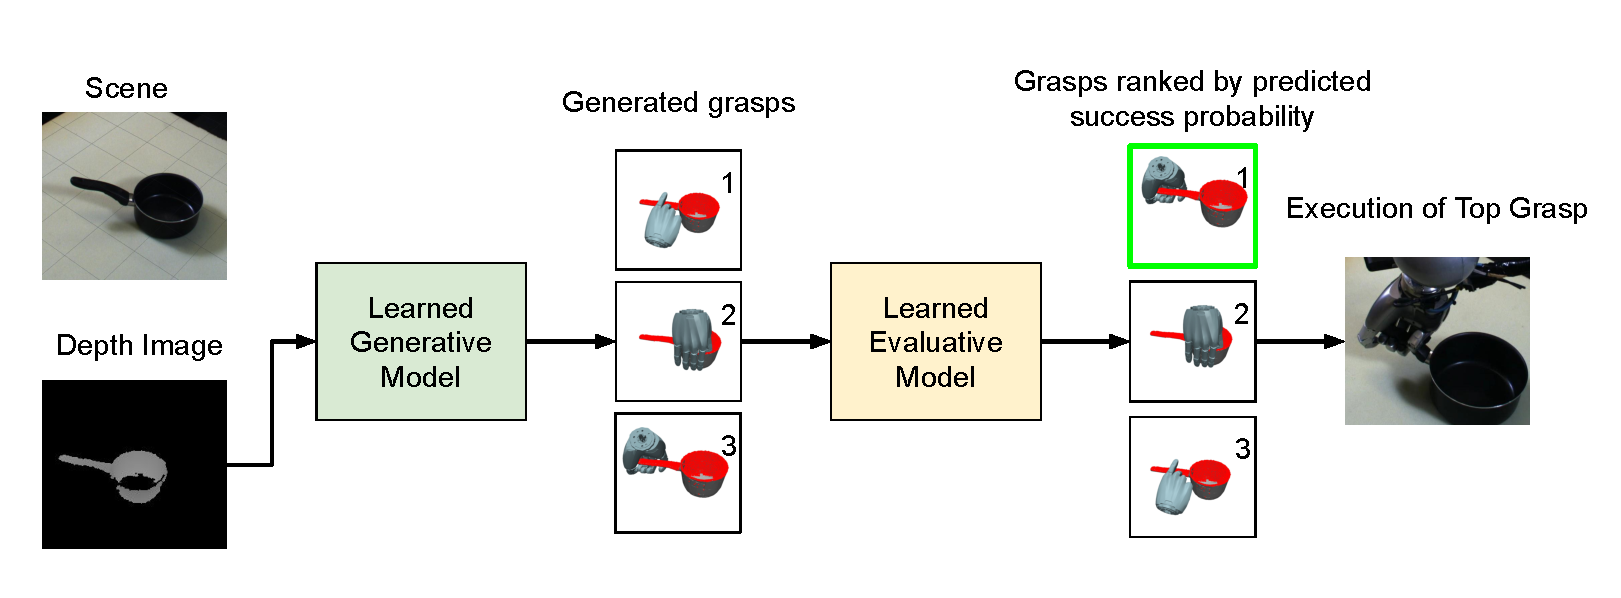
\includegraphics[width=\columnwidth]{images/GEAarchitecture.pdf}
  \end{center}
  \caption{Our grasping architecture. When shown an object, a generative model (GM) produces grasps, ranked according to its likelihood model. These are re-ranked by the predicted success probability of the evaluative Model (EM).The top ranked grasp is executed \label{fig:systemArchitecture}}
\end{figure}

The contributions of this paper are as follows. First, we present a data set of 2.4m simulated dexterous grasps, available to evaluate dexterous grasping algorithms. Second, we release the source code of the dexterous grasp simulator, which can be used to visualise the data set and gather new data.\footnote{The code and simulated grasp data set are available at \href{https://rusen.github.io/DDG}{https://rusen.github.io/DDG}.} Third, we combine an existing learned generative model with multiple learned evaluative models that are trained from simulated grasps proposed by the generative model. Fourth, we present an extensive evaluation of all these models on our simulated data set. Fifth, we compare the two most promising variants on a real robot with a data set of objects in challenging poses. Finally, we perform a deep dive into the simulation results.

The model variants are organised in three dimensions. First, we employ two different generative models (GM1 \cite{kopicki2015ijrr} and GM2 \cite{kopicki2019ijrr}), one of which (GM2) is designed specifically for single view grasping. Second, we use two different back-bones for the evaluative model, VGG-16 and ResNet-50. Third, we experiment with two optimisation techniques--gradient ascent (GA) and stochastic annealing (SA)--to search for better grasps using the evaluative model as an objective function.

%The first contribution of this paper is the first generative-evaluative architecture where both generative and evaluative models are learned. Second, three novel evaluative networks, based on existing VGG-16 and ResNet-50 architectures, were proposed. Finally, a grasp simulation dataset containing 2M+ grasps on 295 objects, along with the simulator code will be released to to the community. In order to simulate the wide range of physical variations that real world objects have, a data set is acquired by simulation of  grasps proposed by the generative models on novel objects. We vary the physical characteristics of the objects in each simulated scene (mass, friction) which the robot can not observe. This dataset was used to train three evaluative neural networks. The evaluative models were then used to rank grasps produced by the generative models (GM1 and GM2) in real robot experiments. 

%The paper builds upon two existing generative grasp models that are learned from a small number of demonstrated grasps using the data-efficient method for LfD. Unlike other approaches to deep grasping, which are restricted to power-grasps, the methods are able to perform a wide variety of grasps, including pinch, rim, power, and handle grasps, and to use additional fingers to provide bracing.

The paper is structured as follows. First, we discuss related work. Second, we describe the design of the grasp simulation, the generation of the data set. Third, the proposed generative evaluative architecture is described and the different architectures employed for the evaluative model are explained, including the optimisation variants of the evaluative model. Fourth, a simulation-based experimental study of the proposed methods is presented. Fifth, we present the real robot study. Finally, we extend the simulation analysis further by examining the inner workings of the best performing model. 


\section{Background and Related Work}

Learning for robot grasping has made steady progress. There are probabilistic machine learning techniques employed for surface estimation for grasping \cite{dragiev2011gaussian}; data efficient methods for learning dexterous grasps from demonstration \cite{ben-amor2012a,kopicki2015ijrr,detry2012a}; logistic regression for classifying grasp features from images \cite{saxena2008a}; and for autonomous learning \cite{detry2010a}. Deep learning is a recent approach to grasping. Most work is for two finger grippers. Approaches either learn an evaluation function for an image-grasp pair \cite{levine16,lenz2015deep,gualtieri2016high,mahler2017dex,pinto2016supersizing,johns2016deep}, learn to predict the grasp parameters \cite{redmon2015real,kumra2017iros} or jointly estimate both \cite{morrison18}. The quantity of real training grasps can be reduced by mixing real and simulated data \cite{bousmalis2017using}. 

A small number of papers have explored deep learning as a method for dexterous grasping. \cite{lu2017planning,varley2015generating,veres2017modeling,zhou20176dof,kappler2015leveraging}. All of these use simulation to generate the training set for learning. Kappler \cite{kappler2015leveraging} showed the ability of a CNN to predict grasp quality for multi-fingered grasps, but uses complete point clouds as object models and only varies the wrist pose for the pre-grasp position, leaving the finger configurations the same. Varley \cite{varley2015generating} and later Zhou \cite{zhou20176dof} went beyond this, each being able to vary the hand pre-shape, and predicting from a single image of the scene. Each of these posed search for the grasp as a pure optimisation problem (using simulated annealing or quasi-Newton methods) on the output of the CNN. They all, also, take the approach of learning an evaluative model, and generate candidates for evaluation uninfluenced by prior knowledge. Veres \cite{veres2017modeling}, in contrast, learns a deep generative model. Finally Lu \cite{lu2017planning} learns an evaluative model, and then, given an input image, optimises the inputs that describe the wrist pose and hand pre-shape to this model via gradient descent, but does not learn a generative model. In addition, the grasps start with a heuristic grasp which is varied within a limited envelope. Of the papers on dexterous grasp learning with deep networks only two approaches \cite{varley2015generating,lu2017planning} have been tested on real grasps, with eight and five test objects each, producing success rates of 75\% and 84\% respectively. An important restriction of both of these methods is that they only plan the pre-grasp, not the finger-surface contacts and are thus limited to power-grasps.

Thus, in each case, either an evaluative model is learned but there is no learned prior over the grasp configuration able to employed as a generative model; or a generative grasp model is learned, but there is no evaluative model learned to select the grasp. Our novelty is thus to bring together a data-efficient method of learning a good generative model with an evaluative model. As with others, we learn the evaluative model from simulation, but the generative model is learned from a small number of demonstrated grasps. 


%n learning to grasp divides into two categories, that we label {\em generative} and {\em evaluative} respectively. We quickly summarise the relationship between this paper and these two.
%
%Generative approaches to grasping include the work of detry et al, kopicki et al, these methods learn distributions of grasps from positive examples. In the case of detry, saxena, these are pinch grasps that are associated with features extracted from monocular or stereo images. Both those pieces of work were restricted to pinch grasps. Both Saxena and Detry require significant training samples, but Detry used real grasps, whereas Saxena used simulation to generate training exemplars. Other approaches use LfD rather than autonomous exploration, as this can significantly reduce the training data required. Peters et al introduced a method for generative grasping by grasp warping, demonstrating an ability to handle new objects of a similar global shape to the training objects. Kopicki et al introduced a factored generative model, showing grasp transfer to novel objects from one example of each grasp type. This is the method than we replicate and build on in our work.
%
%Evaluative approaches to grasping include the work of levine, in which a farm of fourteen robot were used over a two month data gathering period. This data is used to train a neural network that predicts the probability of success of a pinch grasp conditional on an image. In that work the only input is an RGB image, but other approaches to deep grasping tenpas use depth images. However, all these approaches are all data intensive. 
%
%The work that is closest to ours, and the only paper of which we are aware on deep learning applied to dexterous grasping, is that of Hermans et al. 

\section{Data Efficient Learning of a Generative Grasp Model from Demonstration}

%Describe, in new words, the method from IJRR.
This section describes the generative model learning. We employ the method of \citet{kopicki2015ijrr}, which learns a generative model of a dexterous grasp from a demonstration (LfD). That paper posed it as the problem of learning a factored probabilistic model. The method is split into a model learning phase, a model transfer phase, and the grasp generation phase. 

\subsection{Model learning}
The model learning is split into three parts: acquiring an {\em object model}; using this object model, with a demonstrated grasp, to build a {\em contact model} for each finger link in contact with the object; and acquiring a {\em hand configuration model} from the demonstrated grasp. After learning the object model can be discarded.

\subsubsection{Object model}
First, a point cloud of the object used for the demonstrated grasp is acquired by a depth camera, from several views. Each point is augmented with the estimated principal curvatures at that point and a surface normal. Thus, the $j^{th}$ point  in the cloud gives rise to a feature $x_j=(p_j, q_j, r_j)$, with the components being its position $p_j \in \mathbb R^3$, orientation $q_j \in SO(3)$ and principal curvatures $r_j=(r_{j,1},r_{j,2}) \in \mathbb R^2$. The orientation $q_j$ is defined by $k_{j,1},k_{j,2}$, which are the directions of the principal curvatures.  For later convenience we use $v=(p,q)$ to denote position and orientation combined. These features $x_j$ allow the object model to be defined as a kernel density estimate of the joint density over $v$ and $r$.
\begin{equation}
\om(v, r) \equiv \pdf^\om(v, r) \simeq \sum_{j=1}^{K_O} w_j \mathcal{K}(v, r|{x_j}, \sigma_{x})
%RD: mu and sigma are not properly defined.
\label{eq:om}
\end{equation}
where $\om$ is short for $\pdf^\om$, bandwidth $\sigma_{x} = (\sigma_{p}, \sigma _{q}, \sigma_{r})$, $K_O$ is the number of features $x_j$ in the object model, all weights are equal $w_j = 1/{K_O}$, and $\mathcal{K}$ is defined as a product:
\begin{equation}\label{eq:kernel_in_se3}
\mathcal{K}(x | \mu, \sigma) = \mathcal{N}_3(p| \mu_p, \sigma_p) \Theta(q| \mu_q, \sigma_q) \mathcal{N}_2(r| \mu_r, \sigma_r)
\end{equation}
where $\mu$ is the kernel mean point, $\sigma$ is the kernel bandwidth, $\mathcal{N}_n$ is an $n$-variate isotropic Gaussian kernel, and ${\Theta}$ corresponds to a pair of antipodal von Mises-Fisher distributions.
\begin{figure*}[t]
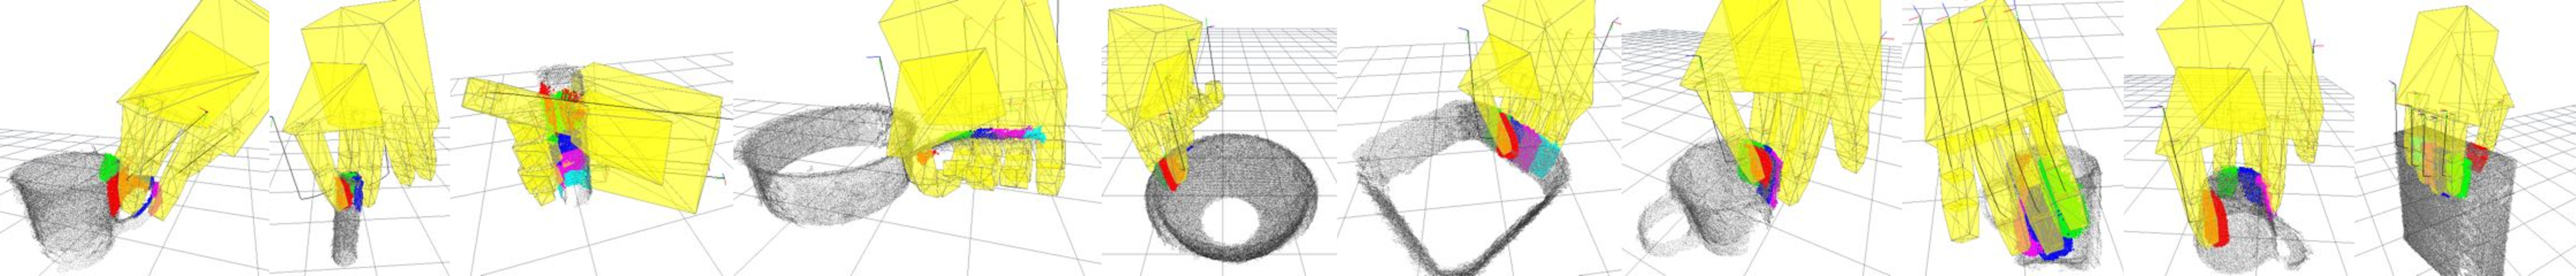
\includegraphics[width=\textwidth]{images/training-examples}
%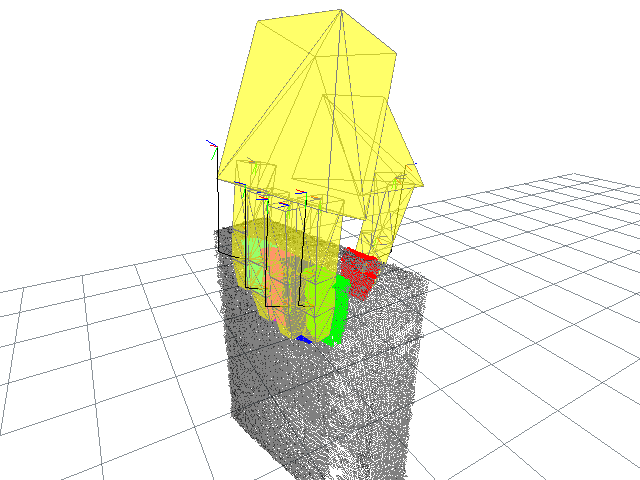
\includegraphics[width=0.1\textwidth]{images/contact-viewall2}
%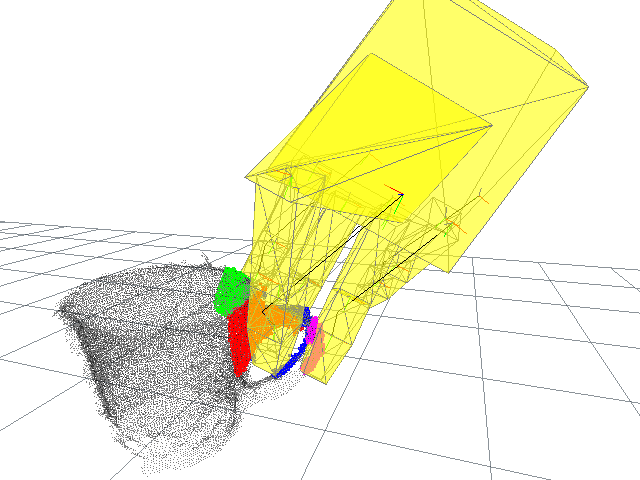
\includegraphics[width=0.1\textwidth]{images/contact-viewall3}
%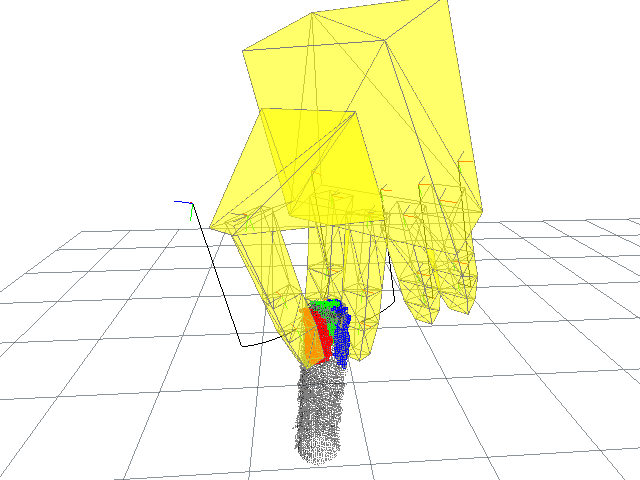
\includegraphics[width=0.1\textwidth]{images/contact-viewall4}
%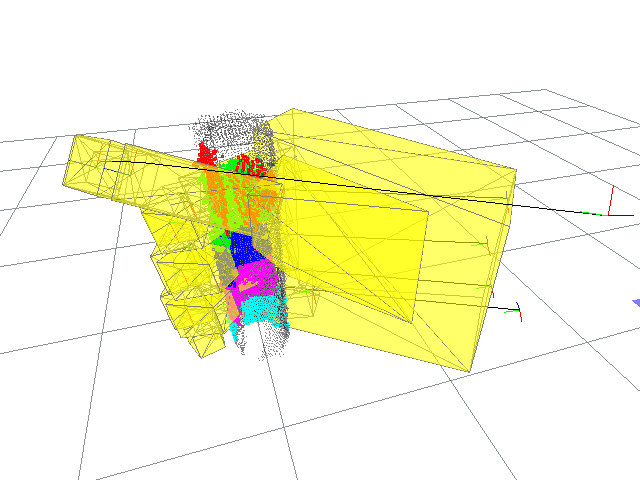
\includegraphics[width=0.1\textwidth]{images/contact-viewall5}
%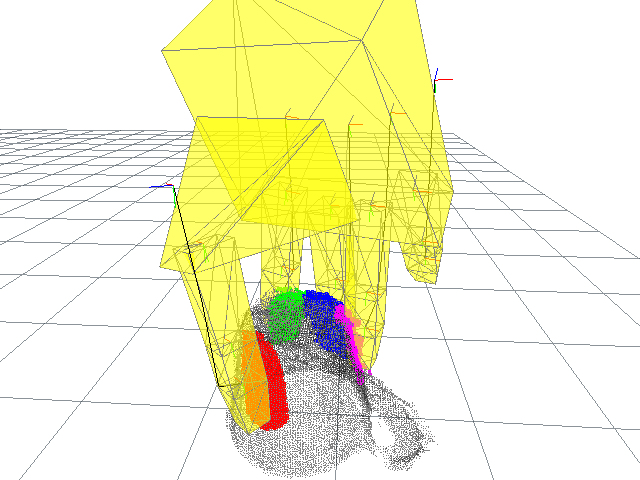
\includegraphics[width=0.1\textwidth]{images/contact-viewall6}
%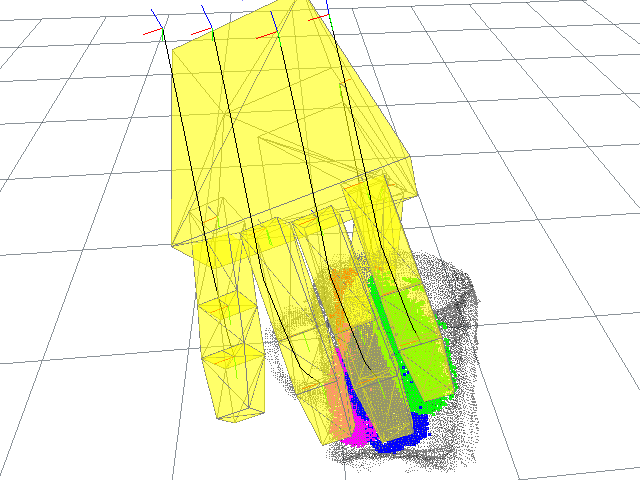
\includegraphics[width=0.1\textwidth]{images/contact-viewall7}
%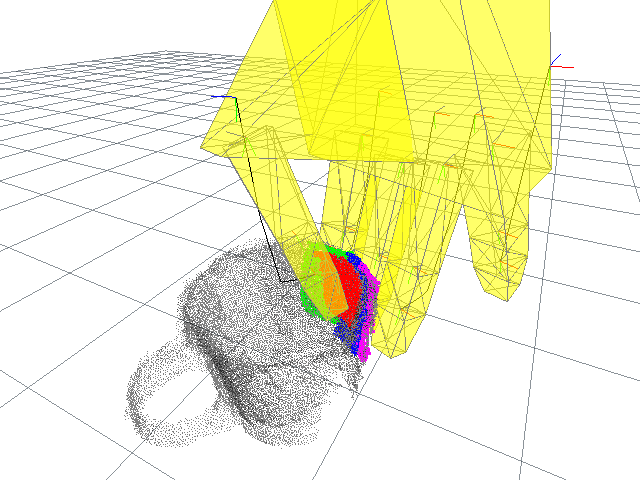
\includegraphics[width=0.1\textwidth]{images/contact-viewall8}
%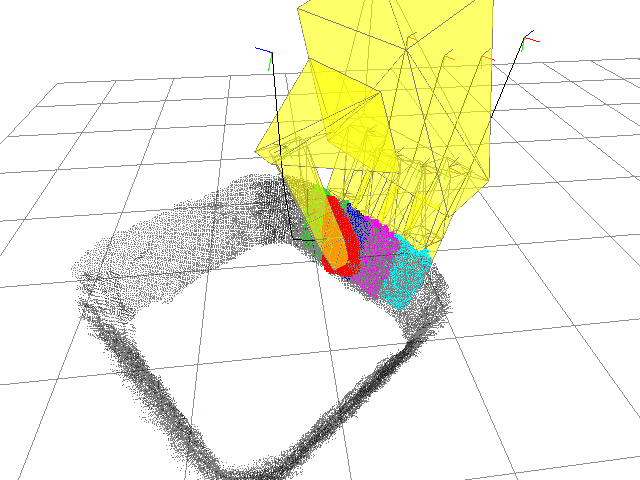
\includegraphics[width=0.1\textwidth]{images/contact-viewall9}
%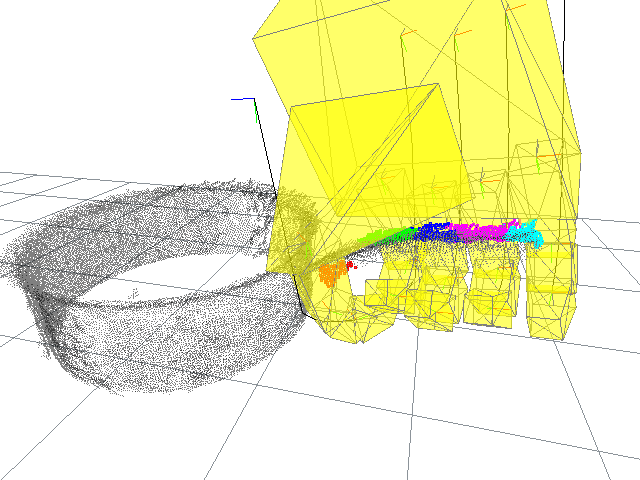
\includegraphics[width=0.1\textwidth]{images/contact-viewall10}
\caption{The ten training grasps for the generative model. The final hand pose is shown in yellow, the sensed point cloud in black, and the parts of the point cloud that contribute to each contact model are coloured by the associated link. \label{fig:generative-training}}
\end{figure*}
\subsubsection{Contact models}
When a grasp is demonstrated the final hand pose is recorded. This is used to find all the finger links $L$ and surface features $x_j$ that are in close proximity. A contact model $M_i$ is built for each finger link $i$. Each feature in the object model that is within some distance $\delta_i$ of finger link $L_i$ contributes to the contact model $\cm_i$ for that link. This contact model is defined for finger link $i$ as follows:
\begin{equation}
\cm_i(u, r) \equiv \pdf^\cm_i(u, r) \simeq \frac{1}{Z} \sum_{j=1}^{K_{M_i}} w_{ij} \mathcal{K}(u, r | {x_j}, \sigma_{x})
%RD: mu and sigma are not properly defined.
\label{eq:cm}
\end{equation}
where $u$ is the pose of $\rl_i$ relative to the pose $v_j$ of the $j^{\mathnormal{th}}$ surface feature, $K_{M_i}$ is the number of surface features in the neighbourhood of link $L_i$, $Z$ is the normalising constant, and $w_{ij}$ is a weight that falls off exponentially as the distance between the feature $x_j$ and the closest point $a_{ij}$ on finger link $L_i$ increases:
\begin{equation}
w_{ij} = \begin{cases}\exp(-\lambda ||p_j-a_{ij}||^2) \quad &\textnormal{ if } ||p_j-a_{ij}|| < \delta_i\\
0 \quad &\textnormal{ otherwise},\end{cases}
\label{eq:learning.modeldist.wgh}
\end{equation}
The key property of a contact model is that it is conditioned on local surface features likely to be found on other objects, so that the grasp can be transferred. We use the principal curvatures $r$, but many local surface descriptors would do. %A contact model can be visualised by marginalising out the dimensions for the rigid body transformation $u$, showing us the distribution over the local curvatures that finger link $L_i$ experienced in the demonstrated grasp. 
%
%\begin{figure*}
%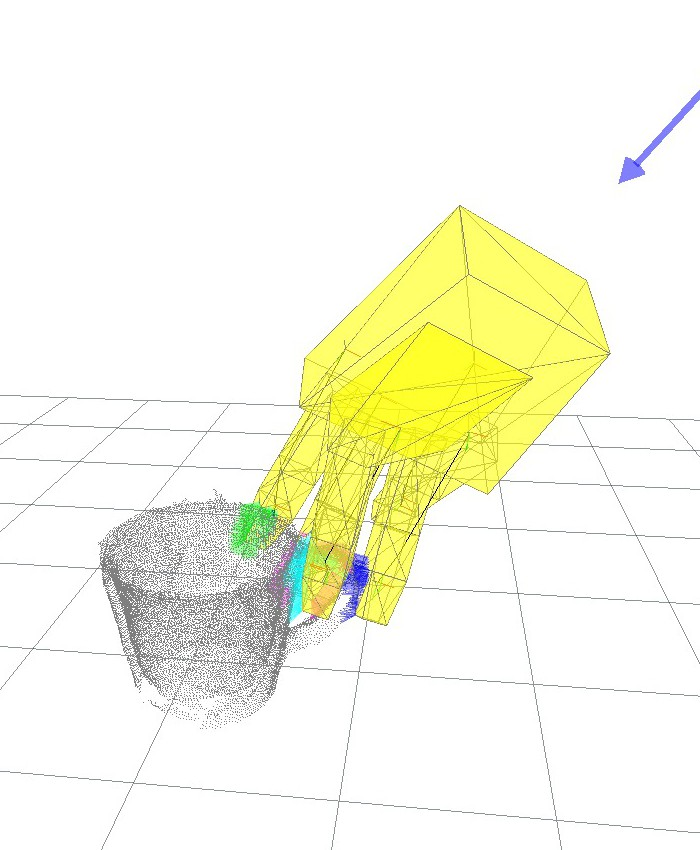
\includegraphics[height=2cm]{images/contact-model-learning/handle-grasp}
%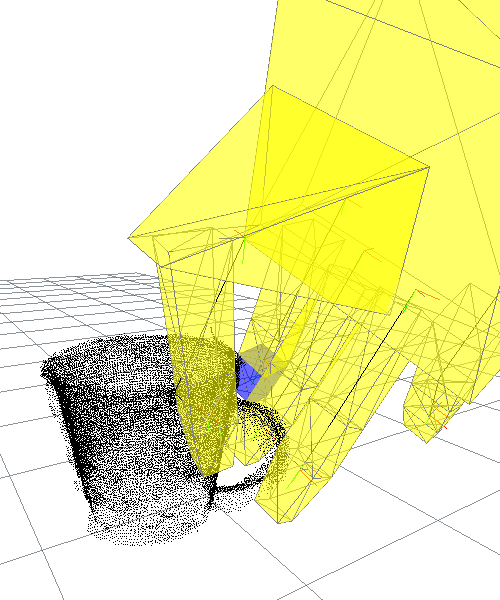
\includegraphics[height=2cm]{images/contact-model-learning/link8}
%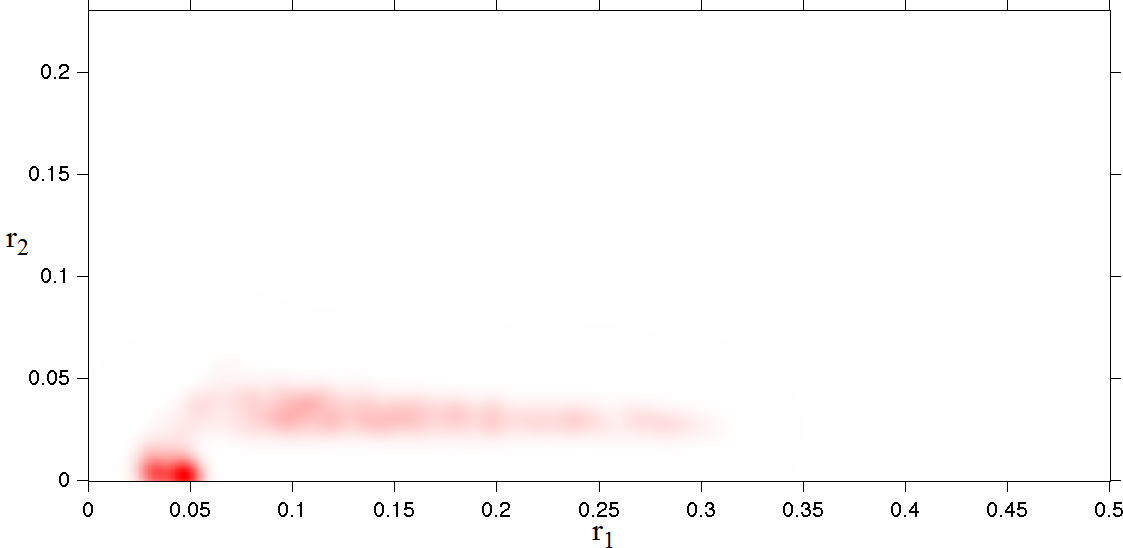
\includegraphics[height=2cm]{images/contact-model-learning/handle_model_08_00778r}
%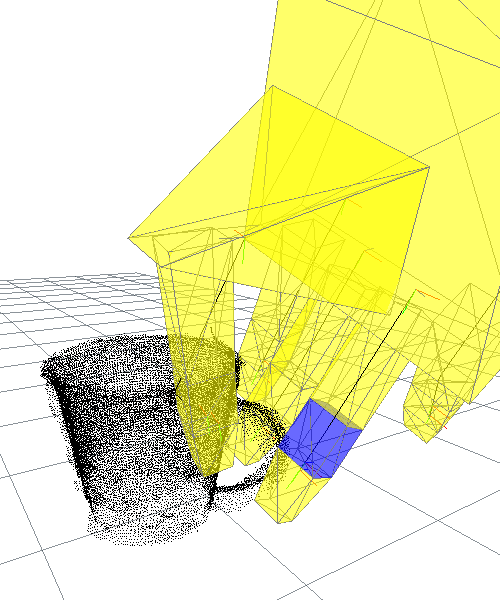
\includegraphics[height=2cm]{images/contact-model-learning/link15}
%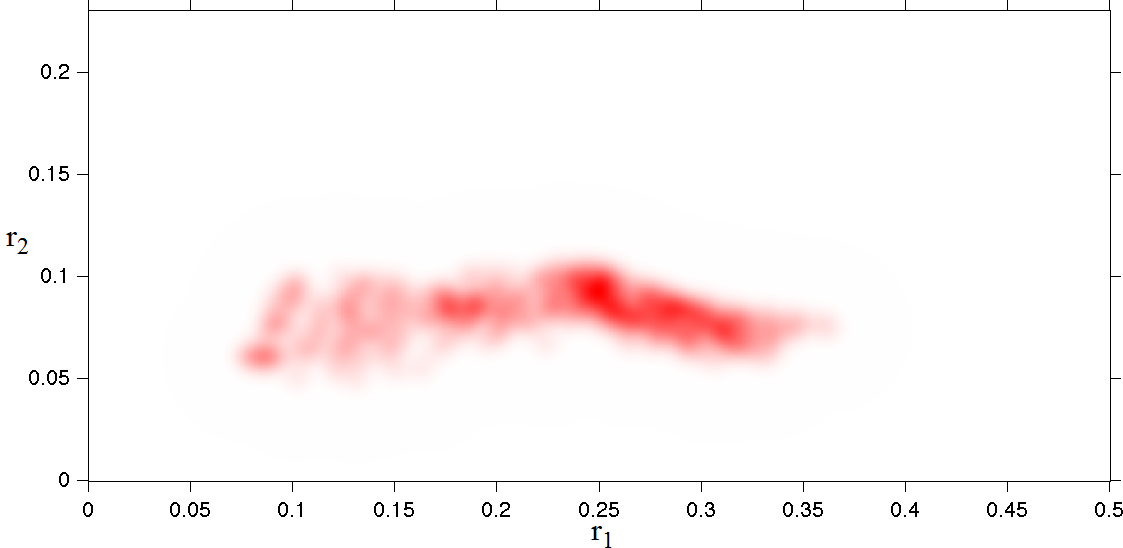
\includegraphics[height=2cm]{images/contact-model-learning/handle_model_15_00329r}
%  \caption{A training grasp and some contact models arising from it.}
%  \label{fig:contactModels}
%\end{figure*}

\subsection{Hand configuration model}
In addition to a contact model for each finger-link, a model of the hand configuration $h_c \in \mathbb R^D$ is recorded, where $D$ is the number of DoF in the hand. $h_c$  is recorded for several points on the demonstrated grasp trajectory as the hand closed. The learned model is:
\begin{equation}
\hc(h_c) \equiv \sum_{\gamma \in [-\beta, \beta]} w({h_c(\gamma)}) \mathcal{N}_D(h_c|h_c(\gamma), \sigma_{h_c}) 
\label{eq:hc}
\end{equation}
where $w({h_c(\gamma)}) = \exp(-\alpha \|h_c(\gamma) - h^g_c \|^2)$; $\gamma$ is a parameter that interpolates between the beginning ($h^t_c$) and end ($h^g_c$) points on the trajectory, governed via \eq\ref{eq:learning.configmodel.config} below; and $\beta$ is a parameter that allows extrapolation of the hand configuration.
\begin{equation}
h_c(\gamma) = (1 - \gamma)h^g_c + \gamma h^t_c
\label{eq:learning.configmodel.config}
\end{equation}
\subsection{Grasp Transfer}
When presented with a new object $o_{new}$ the contact models must be transferred to that object. A partial point cloud of $o_{new}$ is acquired (from a single view) and recast as a density, $\om_{new}$, again using \eq \ref{eq:om}. The transfer of each contact model $\cm_i$ is achieved by convolving $\cm_i$ with $\om_{new}$. This convolution is approximated with a Monte-Carlo method, resulting in an kernel density model of the pose $s$ of the finger link $i$ (in workspace coordinates) for the new object. The Monte-Carlo procedure samples poses for link $L_i$ on the new object. The $j^{th}$ sample is $\hat{s}_{ij}=(\hat{p}_{ij},\hat{q}_{ij})$. Each sample $\hat{s}_{ij}$ is weighted $w_{ij}$ by its likelihood. These samples are used to build what we term the query density:
\begin{equation}
\qd_i(s) \simeq \sum^{K_{Q_i}}_{j=1} w_{ij} \mathcal{N}_3(p|{\hat{p}_{ij}}, \sigma_{p}) \Theta(q|{\hat{q}_{ij}}, \sigma_{q})%, \quad i = 1, ..., N_L
\label{eq:qd.approx}
\end{equation}
where all the weights are normalised, $\sum_j w_{ij} = 1$. A query density is constructed for every contact model and the new object. These query densities, together with the hand configuration model, are then used to generate grasps. Query density computation is fast, taking $<0.5$ second per grasp model.
\begin{figure*}[t]
\begin{center}
  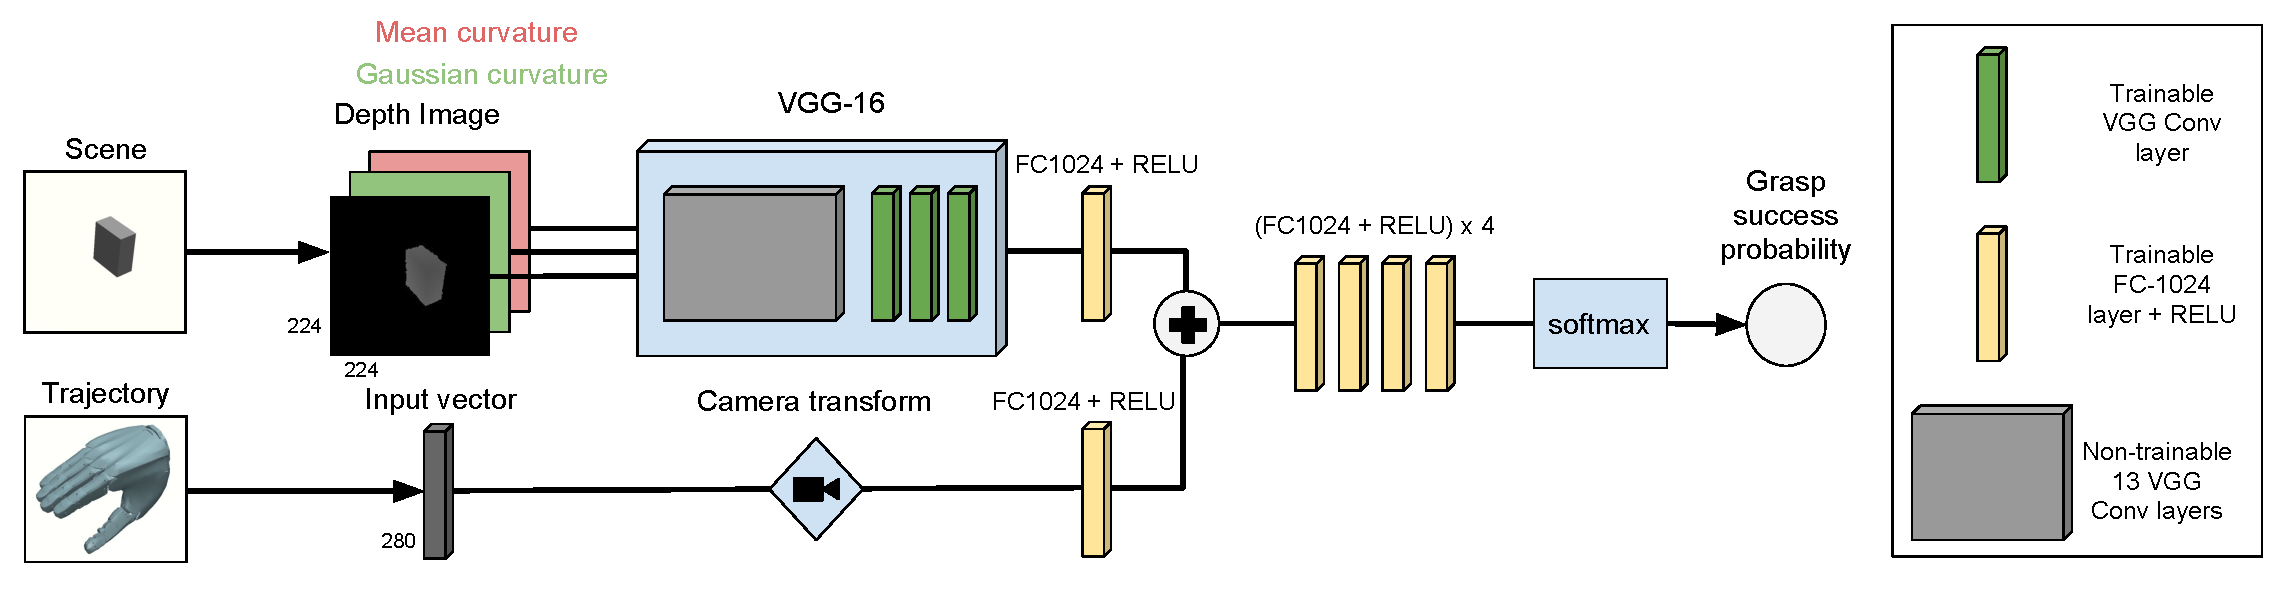
\includegraphics[width=0.9\textwidth]{images/networkArchitecture.pdf}
  \end{center}
  \caption{The evaluative network architecture.}
\label{fig:networkArchitecture}
\end{figure*}
\subsection{Grasp generation}
Candidate grasps may be generated as follows. Select a query density $k$ and take a sample  $s_k \sim \qd_{k}$. Then, take a sample $h_c \sim C$ from the hand configuration model. This pair of samples together define, via the hand kinematics, a complete grasp $h=(h_w,h_c)$, where $h_w$ is the pose of the wrist and $h_c$ is the configuration of the hand. The initial grasp is then improved by stochastic hill-climbing on a product of experts:
\begin{equation}
\argmax{(h_w, h_c)} \hc(h_c) \prod_{\qd_i \in \mathcal{Q}} \qd_i\left(k_{i}^{\mathrm{for}}\left(h_w, h_c\right)\right)
\label{eq:grasping.product}
\end{equation}
This generate and improvement process has periodic pruning steps, in which only the higher likelihood grasps are retained. It can be run many times, thus enabling the generation of many candidate grasps. In addition, a separate generative model can be learned for each demonstrated grasp. Thus, when presented with a new object, each grasp model can be used to generate and improve grasps. We generate and optimise 100 grasps per grasp type. Finally, the many candidate grasps generated from each grasp model can be compared and ranked according to their likelihoods. The product of experts formulation, however, only ensures that the generated grasps have high likelihood according to the model. There is no estimate of the probability that the grasp will succeed. This motivates the dual architecture in this paper. We now turn to the learning method we used to re-rank the grasps according to predicted success probability. 

\subsection{Training Grasps for Our Study}

For the purposes of our study, ten example grasps were provided. These are visualised in Figure~\ref{fig:generative-training}. In contrast to \cite{kopicki2015ijrr}, although seven views of each training object were taken, we trained a separate generative model for each view. This led to a total of 70 generative models being learned, one for each grasp-view combination. In addition, we made two innovations to the generative model. In the first, because of the view based training, we filter surface normals on the object model so that for each contact model we only consider points on the object surface with surface normals within +/- 90 degrees of the surface of the finger link. In the second, rather than globally selected the best grasps during optimisation---regardless of the training grasp type, as in the algorithm reported in \cite{kopicki2015ijrr}---we select half globally across all training grasp types, and half we force to be evenly spread across the grasp types. This enables us to keep a broad range of grasp options open to us for evaluation, and thus improves performance.
 \label{section:generative}

\section{Improved Generative Learning}

%Describe, in new words, the method from IJRR.
%% This section describes the improved generative method. Only the differences between the original method (given in the previous section) and the new methhod are explained here. 

In this paper we also utilised a more advanced generative model, which we refer to as GM2. This model has four features which are different from the base model GM1. As for GM1 these are not a contribution of this paper and are described fully in \cite{kopicki2019ijrr}. For completeness we briefly describe the three differences between GM2 and GM1. 

\subsection{Object View Model}\label{sec:representations.object}
The first difference is that the learning of grasp models is done per view, rather than per grasp. This means that for a training grasp made on an object viewed from seven viewpoints that there will be seven grasp models learned. This enables grasps to generalise better when the testing object to be grasped is thick and is only seen from a single view. The view based models allow a greater role to be played by the hand shape model and this enables generated grasps to have fingers which `float' behind a back surface that cannot be seen by the robot.

\subsection{Clustering Contact Models}\label{sec:learning.clustering}

The second innovation is the ability to merge grasp models learned from different grasps. Using the memory based scheme of GM1, the number of contact models $N_{\mathcal{M}}$ equals the product of the number of training grasps by the number of views. This has two undesirable properties. First, it means that generation of grasps for test objects rises linearly in the number of training grasps. Second, it limits the generalisation power of the contact models. We can overcome both these problems by clustering the contact models from each training grasp. To do this we need a measure of the similarity between any pair of contact models. Recall that our contact models are probability densities represented as kernel density estimators. Thus, we need a distance metric in the space of probability densities of a given dimension.

One possibility would to employ Jensen-Shannon distance, but this is slow to evaluate. We therefore start by devising a simple asymmetric divergence, which is designed to be quick to compute. We then build on top of it a symmetric distance. Having obtained this distance measure we can employ our clustering method of choice, which in our case was affinity propagation \cite{frey2007clustering}. After clustering, we compute a cluster prototype as described in \cite{kopicki2019}.

\subsection{Improved Grasp Transfer and Inference}
GM2 utilises the same distance measure to transfer grasps when creating the query densities and also to evaluate candidate grasps. This has the effect of making the proposed grasps more conservative and thus closer to the demonstrated grasps in terms of the type of contacts made with the target object.

Having described both generative models we now proceed to describe how we use these to generate a data-set of 2 million simulated dexterous grasps. \label{section:generative_new}

% \section{The Evaluative Model} \label{section:learning}

% The generative model generates 1000 grasps for a new object within 15 seconds on a 2x Intel Xeon E5-2650 v2 Eight Core 2.6GHz. There is, however, no estimate of the probability of grasp success. This the purpose of the evaluative model. Deep networks have been shown to learn good evaluative models of grasp success for two finger grippers and for dexterous hands (Barrett, Allegro) performing power grasps.  
%In this section, our evaluative deep network architecture is described. In the following section, the simulation used to generate the training data is detailed.
%First, the generative model largely ignores global information about the object; relying instead on global information about the hand shape, and local information about finger-object contacts. To predict grasp success probability we need a learner that somehow takes into account global information, such as global shape, mass, mass distribution, friction coefficients, deformability, etcetera. The difficulty with this is that, given a single depth image, the learner does not have direct access to these. Thus, they cannot be estimated, but all that can be learned is the association Second, the 

%It is time-consuming and expensive to collect real grasp data with using robotic arms with dexterous hands. Unlike gripper + arm combinations which require relatively less supervision \cite{Levine1}, dexterous hands can be much more fragile due to their complexity. Advances in physics simulators have made it possible to re-create robotic experiment setups in simulation. We created a simulated experimental setup in order evaluate grasp, which allowed us to collect as much data as needed in a short period of time with no supervision.
We now present the architecture (Figure~\ref{fig:networkArchitecture}) of our evaluative network $f(I_t, h_t)$, where $I^t$ is a colourized depth image of the object, and $h_t = (h_{tw}, h_{tc})$ gives the sequence of wrist poses and hand configurations for a grasp, expressed in the camera frame. The network outputs a grasp success probability for image-grasp pair $I_t$, $h_t$. Section~\ref{section:simulation} gives details of the simulation used to generate the training data.

% The purpose of the network is to learn the relationship between the point cloud, given as a colorized depth image, and grasp (hand shape) parameters which encode the configuration of the hand with respect to the camera frame. This is a complex task, as the kinematic model of the hand is unknown to the network, and it has to consider each grasp as a black box: The network knows the inputs that configure the hand, including the joint positions, and only has access to the outcome in the form of success/failure. 
% Talk more about the architecture
For visual processing, we use the VGG-16 network pre-trained on ImageNet. The final three layers are fine-tuned, while the first 13 layers are frozen. Pre-processing segments the table plane from the object point cloud of the object. The segmented $640 \times 480$ depth image $I_{t}^{depth}$ is cropped to a window of $460 \times 460$, located in the image centre. Then, it is down-sampled to $224 \times 224$. The colourization creates a $224 \times 224$ 3-channel image $I_t$. The channels  are the mean curvature, the Gaussian curvature, and the depth. %The formula of mean curvature is $h = {gr}_{xx} + {gr}_{yy}$, where ${gr}_{xx}$ is the second gradient in horizontal direction in a $1 \times 3$ window, and ${gr}_{yy}$ is its vertical counterpart. Similarly, Gaussian curvature $k = {gr}_{xx} \times {gr}_{yy} - ({gr}_{xy})^2$.
The hand trajectory $h_t$ comprises 10 way-points, each of 28 dimensions (20 for the finger joint angles, 1 for the grasp type, and 7 for the wrist pose), giving 280 dimensions. This is transformed to 1024 using a single layer. This and the output of the final VGG layer are added together unit-wise. Then there are four fully connected layers each comprising 1024 RELU nodes. The output is a grasp success/failure probability, encoded by two softmax nodes.  We train using the cross-entropy loss function:
\begin{equation}
H_{y'}(y) := - \sum_{i} ({y_i' \log(y_i) + (1-y_i') \log (1-y_i)})
\label{equation:crossentropy}
\end{equation}
where $y_i'$ is the ground truth success (1) or failure (0); $y_i = f(I_i, h_i)$ is the predicted grasp success of grasp trajectory $h_i$, and $I_i$ is the associated colourized depth image of grasp $h_i$.
\begin{figure}
\begin{center}
  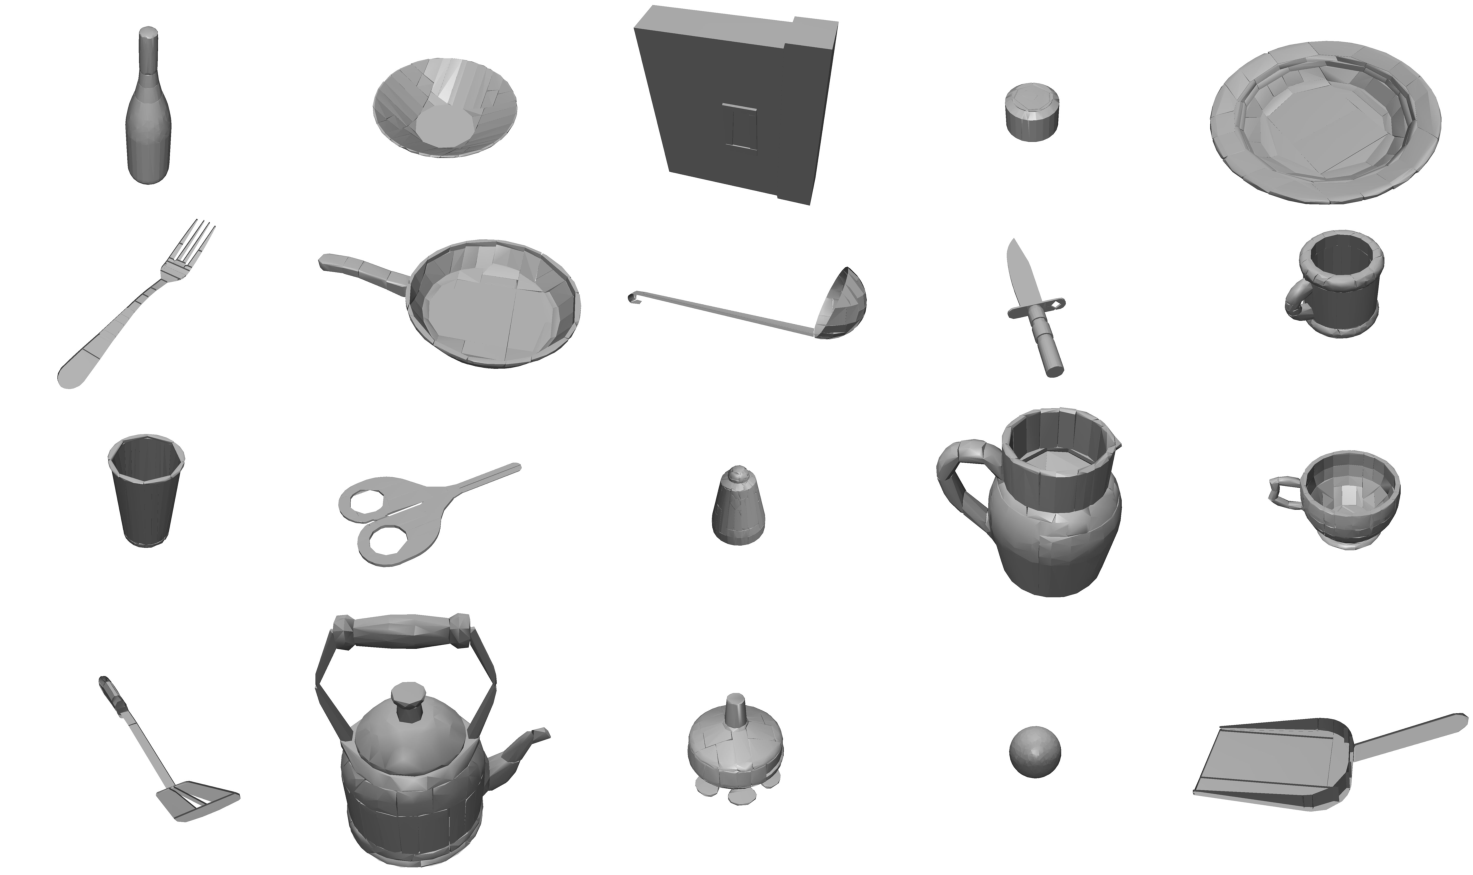
\includegraphics[width=0.9\linewidth]{images/allObjects-small.pdf}
  \end{center}
  \caption{Sample objects from all classes in the 3D model dataset.}
  \label{fig:allObjects}
\end{figure}
We trained our network on a data set of 441,312 grasps. We now describe the simulation used to generate a realistic training set. % o 7000 distinct scenes, where each scene contains a random instantiation of one of the objects in the dataset with varying rigid body transformations applied, as well as friction and weight changes. The network was tested on 80000 grasps on 1200 scenes of unseen objects, as well as real robot experiments, as explained in Section \ref{section:experiments}. In order to make a direct comparison with Kopicki et al. \cite{kopicki2015ijrr}, we pick top grasps based on both the original ranking, as explained in Section \ref{section:generative}, and according to the predicted success probabilities by the network. 

%We opted to use a grasp success prediction network due to the fact that the grasp generator function, explained in the previous chapter, provides alternatives of most intuitive types of grasps. A logical extension of this work would be to pair our learning algorithm with a grasp generator network, which we consider as future work.

%Overall network architecture. VGG summary. Description of new layers. Representation of hand parameters, frames of reference, camera image conversion for VGG, trajectory of wrist and fingers.



\section{The Simulated Grasp Data Set}
\label{section:simulation}
%Introductory sentences here
In this section, we describe how we generated a realistic simulated data set for dexterous grasping. This captures variations in both observable (e.g. object pose) and unobservable (e.g. surface friction) parameters.

To generate the training set a simulated depth image of a scene containing a single unfamiliar object is generated. Using either of the generative models GM1 or GM2, grasps are generated and executed in simulation. The success or failure of each simulated grasp is recorded. Producing a good simulation for evaluating grasps is non-trivial. An important problem is that the data set must capture the natural uncertainty in unobservable variables, such as mass and friction. Since many of these parameters are unobservable we are thus creating a data set such that the grasp policy must work across a range of variations. This is thus a form of {\em domain randomisation}. A similar technique has been employed by \cite{mahler2017dex}, but we extend it from a single grasp quality metric to full rigid body simulation.

\subsection{Features and Constraints of the Virtual Environment}
\label{subsection:environment}

The collected 3D model dataset contains 294 objects from 20 classes, namely, bottles, bowls, cans, boxes, cups, mugs, pans, salt and pepper shakers, plates, forks, spoons, spatulas, knives, teapots, teacups, tennis balls, dustpans, scissors, funnels and jugs (Figure \ref{fig:allObjects}). All objects in the dataset can be grasped using the DLR-II hand, although there are limitations on how some object classes can be approached. For example, teapots and jugs are not easy to grasp except by their handles due being larger than the hand's maximum aperture, while small objects such as salt and pepper shakers can be approached in more creative ways. The number of objects in each class varies from 1 (dustpan) to 25 (bottles). Long/thin objects such as kitchen utensils are placed vertically in a short, heavy stand in order to make them graspable without touching the table. This reflects the real-world scenario, as attempting to grasp a spatula lying on a table would be dangerous for the robotic hand. In total, 250 objects from all 20 classes were allocated for training and validation, while the remaining 44 objects from 19 classes belong to the test set.

We employ MuJoCo \cite{MuJoCo} as the rigid-body simulator. Due to the fact that collision checking in MuJoCo requires that objects comprise convex parts, all 294 objects were decomposed into convex parts using V-HACD algorithm \cite{V-HACD}. The number of sub-parts varies from 2 to 120.

During the scene creation, the object is placed on the virtual table at a pseudo-random pose. Most objects are placed in a canonical upright pose, and only randomly rotated around the gravity axis (akin to being placed on a turntable). The objects belonging to the mug and cup classes have fully random 3D rotations applied before they are placed on the table, since it is possible to grasp them in almost any setting using the robot hand.

\begin{figure}
  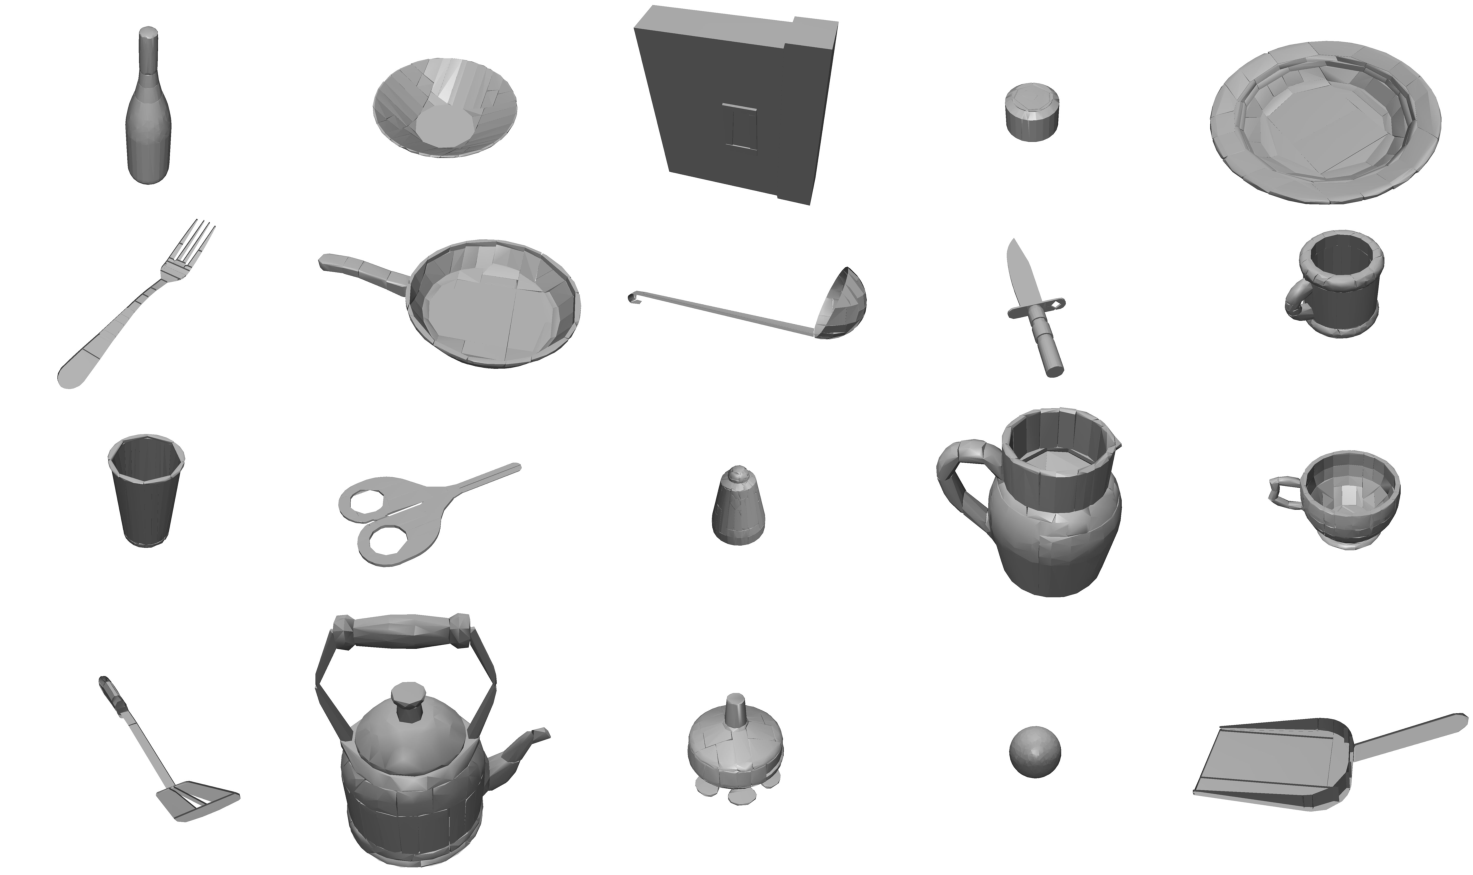
\includegraphics[width=\linewidth]{images/allObjects-small.pdf}
  \caption{A sample of the 294 objects drawn from the 20 object classes.
  \label{fig:allObjects}}
\end{figure}

To achieve domain randomisation, prior distributions for mass, size and frictional coefficient were estimated from real-world data. The properties of simulated objects are sampled from these priors. For each object its mean size, mass and friction coefficient are matched to a real counterpart. For each trial, the size is randomly scaled by a factor in the range [0.9,1.1], while remaining within the grasp aperture of the hand. Object mass is uniformly sampled from a category specific range, estimated from real objects (Table~\ref{fig:weights}). The friction coefficient of each object is sampled from a range of $[0.5, 1]$ in MuJoCo default units, intended to simulate surfaces from low-friction (metal) to high-friction (rubber). This variation is critical to ensuring that the evaluative model will predict the robustness of a grasp to unobservable variations.
\begin{table}[]
\centering
\caption{Mass ranges for each object class (grams).}
\label{fig:weights}
\resizebox{\linewidth}{!}{\begin{tabular}{|l|l|l|l|l|l|l|}
\hline
Bottle & Bowl     & Box     & Can     & Cup    & Fork    & Pan     \\ \hline
30-70  & 50-400   & 50-500  & 200-400 & 30-330 & 40-80   & 150-450 \\ \hline
Plate  & Scissors & Shaker  & Spatula & Spoon  & Teacup  & Teapot  \\ \hline
40-80  & 50-150   & 100-160 & 40-80   & 40-80  & 150-250 & 500-800 \\ \hline
Jug    & Knife    & Mug     & Funnel  & Ball   & Dustpan &         \\ \hline
80-200 & 50-150   & 250-350 & 40-80   & 50-70  & 100-150 &         \\ \hline
\end{tabular}}
\end{table}
 
For depth image simulation the Carmine 1.09 depth sensor installed on the robot is simulated with a modified version of the Blensor Kinect sensor simulator \cite{KinectSimulator}. For each object, we vary the camera orientation and distance from the object, as well as object mass, friction, scale, location and orientation. In order to account for calibration errors in the real world setup, we add a small three-dimensional positional noise to each point in the sensor output.

A 3D mesh-model of the DLR-II hand has been used in the simulator. There are no kinematic constraints on how the hand may grasp an object, other than collisions with the table. To ensure realism, we use impedance control for the hand.
%The reasons for the most critical of these decisions are now given in slightly more detail. First, in order to create a realistic simulation environment, we chose the MuJoCo \cite{MuJoCo} physics simulator over other simulators (OpenSim, BulletPhysics, ODE, NVIDIA PhysX) for two reasons: 
%\begin{itemize}
%\item MuJoCo uses generalized coordinates and optimization-based contact dynamics, resulting in fewer numerical instabilities,
%\item MuJoCo is optimized for the quality of physics as well as its speed, hence improving the quality of the physics simulation.
%\end{itemize}
\begin{figure}
  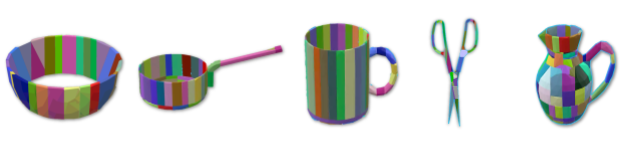
\includegraphics[width=\linewidth]{images/decomposition.png}
  \caption{Approximate convex decomposition of some objects in our dataset. Best viewed in colour.}
  \label{fig:objectDecomposition}
\end{figure}

Some classes are easier to grasp than others. Table \ref{fig:graspperf} shows the success rates of the generated grasps in each class, when attempted with the grasps ranked by the Generative Model (GM1). The sampled grasps perform well on a number of classes including Dustpans, Scissors, Spoons, and Mugs. Some objects can only be grasped in certain ways, i.e. not all 10 training grasps are applicable to all objects.

\begin{table}[]
\centering
\caption{The average and \textbf{top} grasp success rates of GM1 on simulated data.}
\label{fig:graspperf}
\resizebox{\linewidth}{!}{\begin{tabular}{|l|l|l|l|l|l|l|}
\hline
Bottle & Bowl     & Box     & Can     & Cup    & Fork    & Pan     \\ \hline
35.5 - \textbf{47.7}\% & 26.4 - \textbf{61.2}\%   & 16.5 - \textbf{30.1}\%  & 41.4 - \textbf{92.6}\% & 44.7 - \textbf{59.9}\% & 59.6 - \textbf{68.1}\%   & 37.9 - \textbf{57.3}\% \\ \hline
Plate  & Scissors & Shaker  & Spatula & Spoon  & Teacup  & Teapot  \\ \hline
50.2 - \textbf{95.5}\%  & 62.7 - \textbf{69.9}\%   & 47.3 - \textbf{53.3}\% & 57.4 - \textbf{65.7}\%   & 63.4 - \textbf{82.4}\%  & 48.2 - \textbf{91.2}\% & 26.9 - \textbf{23.9}\% \\ \hline
Jug    & Knife    & Mug     & Funnel  & Ball   & Dustpan & \textbf{Total}      \\ \hline
24.9 - \textbf{43.9}\% & 58.3 - \textbf{65.0}\%   & 40.7 - \textbf{80.9}\% & 52.3 - \textbf{65.9}\%   & 28.0 - \textbf{82.8}\%  & 60.1 - \textbf{78.8}\% & 45.8 - \textbf{63.2}\%        \\ \hline
\end{tabular}}
\end{table}

\subsection{Data Collection Methodology}
\label{subsection:dataCollection}

The data set is divided into units called \textit{scenes}, where each scene comprises a single object placed on a table. This object has a specific set of physical parameters, chosen as described below. Many views and grasps are attempted per scene. Below, we specify the time flow of data collection:

\begin{enumerate}
\item A novel instance of an object from the dataset is generated and placed on a virtual table. Variations are applied to object pose, scale, mass, and friction coefficients.
\item A simulated camera takes a depth image $I_s$ of the scene, converted to a point cloud $P_s$. The viewpoint ${elevation}_s$ of the view point is from 30-57 degrees. The ${azimuth}_s$ is sampled from $[0, 2\pi]$. 
\item The positions of all points in the point cloud $P_s$ are shifted by a three-dimensional noise vector sampled from a Gaussian distribution with parameters $\mu=0$ and $\sigma = 0.004$ (unit: meter).
\item Given $P_s$, the chosen generative model (GM1 or GM2) proposes the candidate grasps. For GM1, up to100 grasps are selected. These are the 10 grasps that are highest ranked by the GM for each of the 10 training grasps. For GM2, we select a maximum of 500 grasps: up to 50 grasps from each training grasp.
\item The grasps are applied to the object in simulation.
\item 19 further simulated depth images are taken from other viewpoints around the object, as explained in step 2. Images with fewer than 250 depth points are discarded. We then sample with replacement from the remaining images and associate each sampled image and viewpoint with a grasp created in step 3.
\item The grasp outcome, trajectory and depth image are stored for each trial. The grasp parameters are converted to the camera frame for the associated view.
\end{enumerate}

%Each candidate grasp $h_i = \{w_0, ..., w_{n}\}$ consists of a series of 10 waypoints along : $w_0$, ..., $w_{n}$. A waypoint $w_k$ is a 27-element vector that specifies full configuration of the hand in joint space: 3 dimensions for 3D coordinates and 4 dimensions for the orientation of the wrist, and 20 parameters specifying each finger joint's activation. 
%After a grasp $h_i$ is generated in world coordinates, the waypoints that belong to the grasp are converted to the camera's frame of reference. 
%The goal of our network architecture is to learn which grasps are more likely to succeed given a point cloud, where both input channels are represented in terms of the camera frame of reference. %This point differentiates us from the work of Levine et al. \cite{Levine1}, where camera coordinates are not used. It should be noted that the possible camera locations in our simulated data covers a larger space, with full circular movement $[0, 2\pi]$ on azimuth and $[30-57]$ range in elevation. Our scenes do not have any distinguishing landmarks such as a bin or robot base, which may aid the network in locating the camera in the scene. 

In each scene $S_i$, a number of depth images are taken $\{I_{ik}\}_{k=0}^{20}$, in the manner explained above. The first image $I_{i0}$ is used to generate grasps, as explained in Section \ref{section:generative}. We typically perform 10-500 grasps per scene. Attaching different views to each grasp instead of the seed image $I_{i0}$ ensures there is more variation in terms of viewpoints, resulting in a richer dataset. Typically, performing a grasp takes half the time it takes to acquire an image using the simulated camera.

Once a grasp is performed in simulation, it is considered a success if an object is lifted one metre above the table, and held there for two seconds. If the object slips from the hand during lifting or holding, the grasp is a failure. 

\begin{figure}[t]
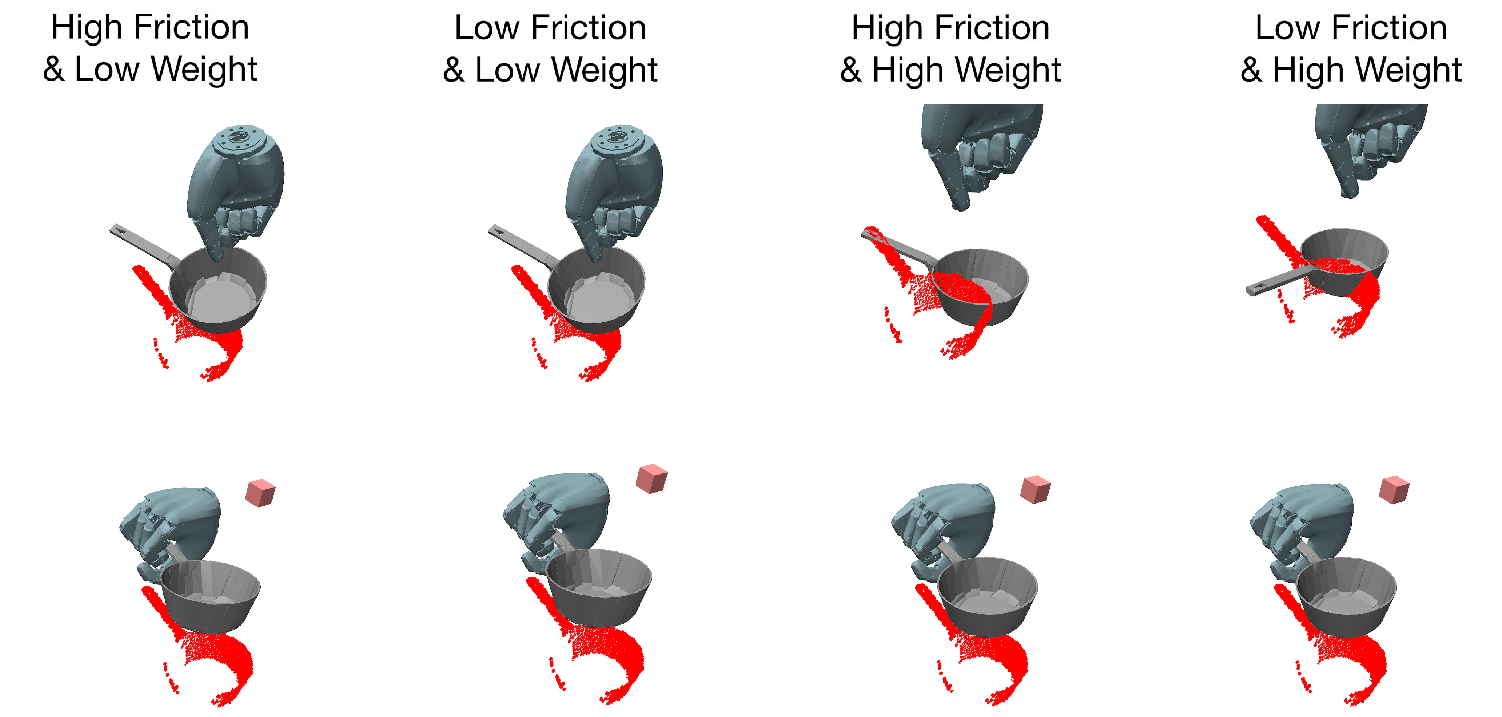
\includegraphics[width=\columnwidth]{images/frictionweight}
%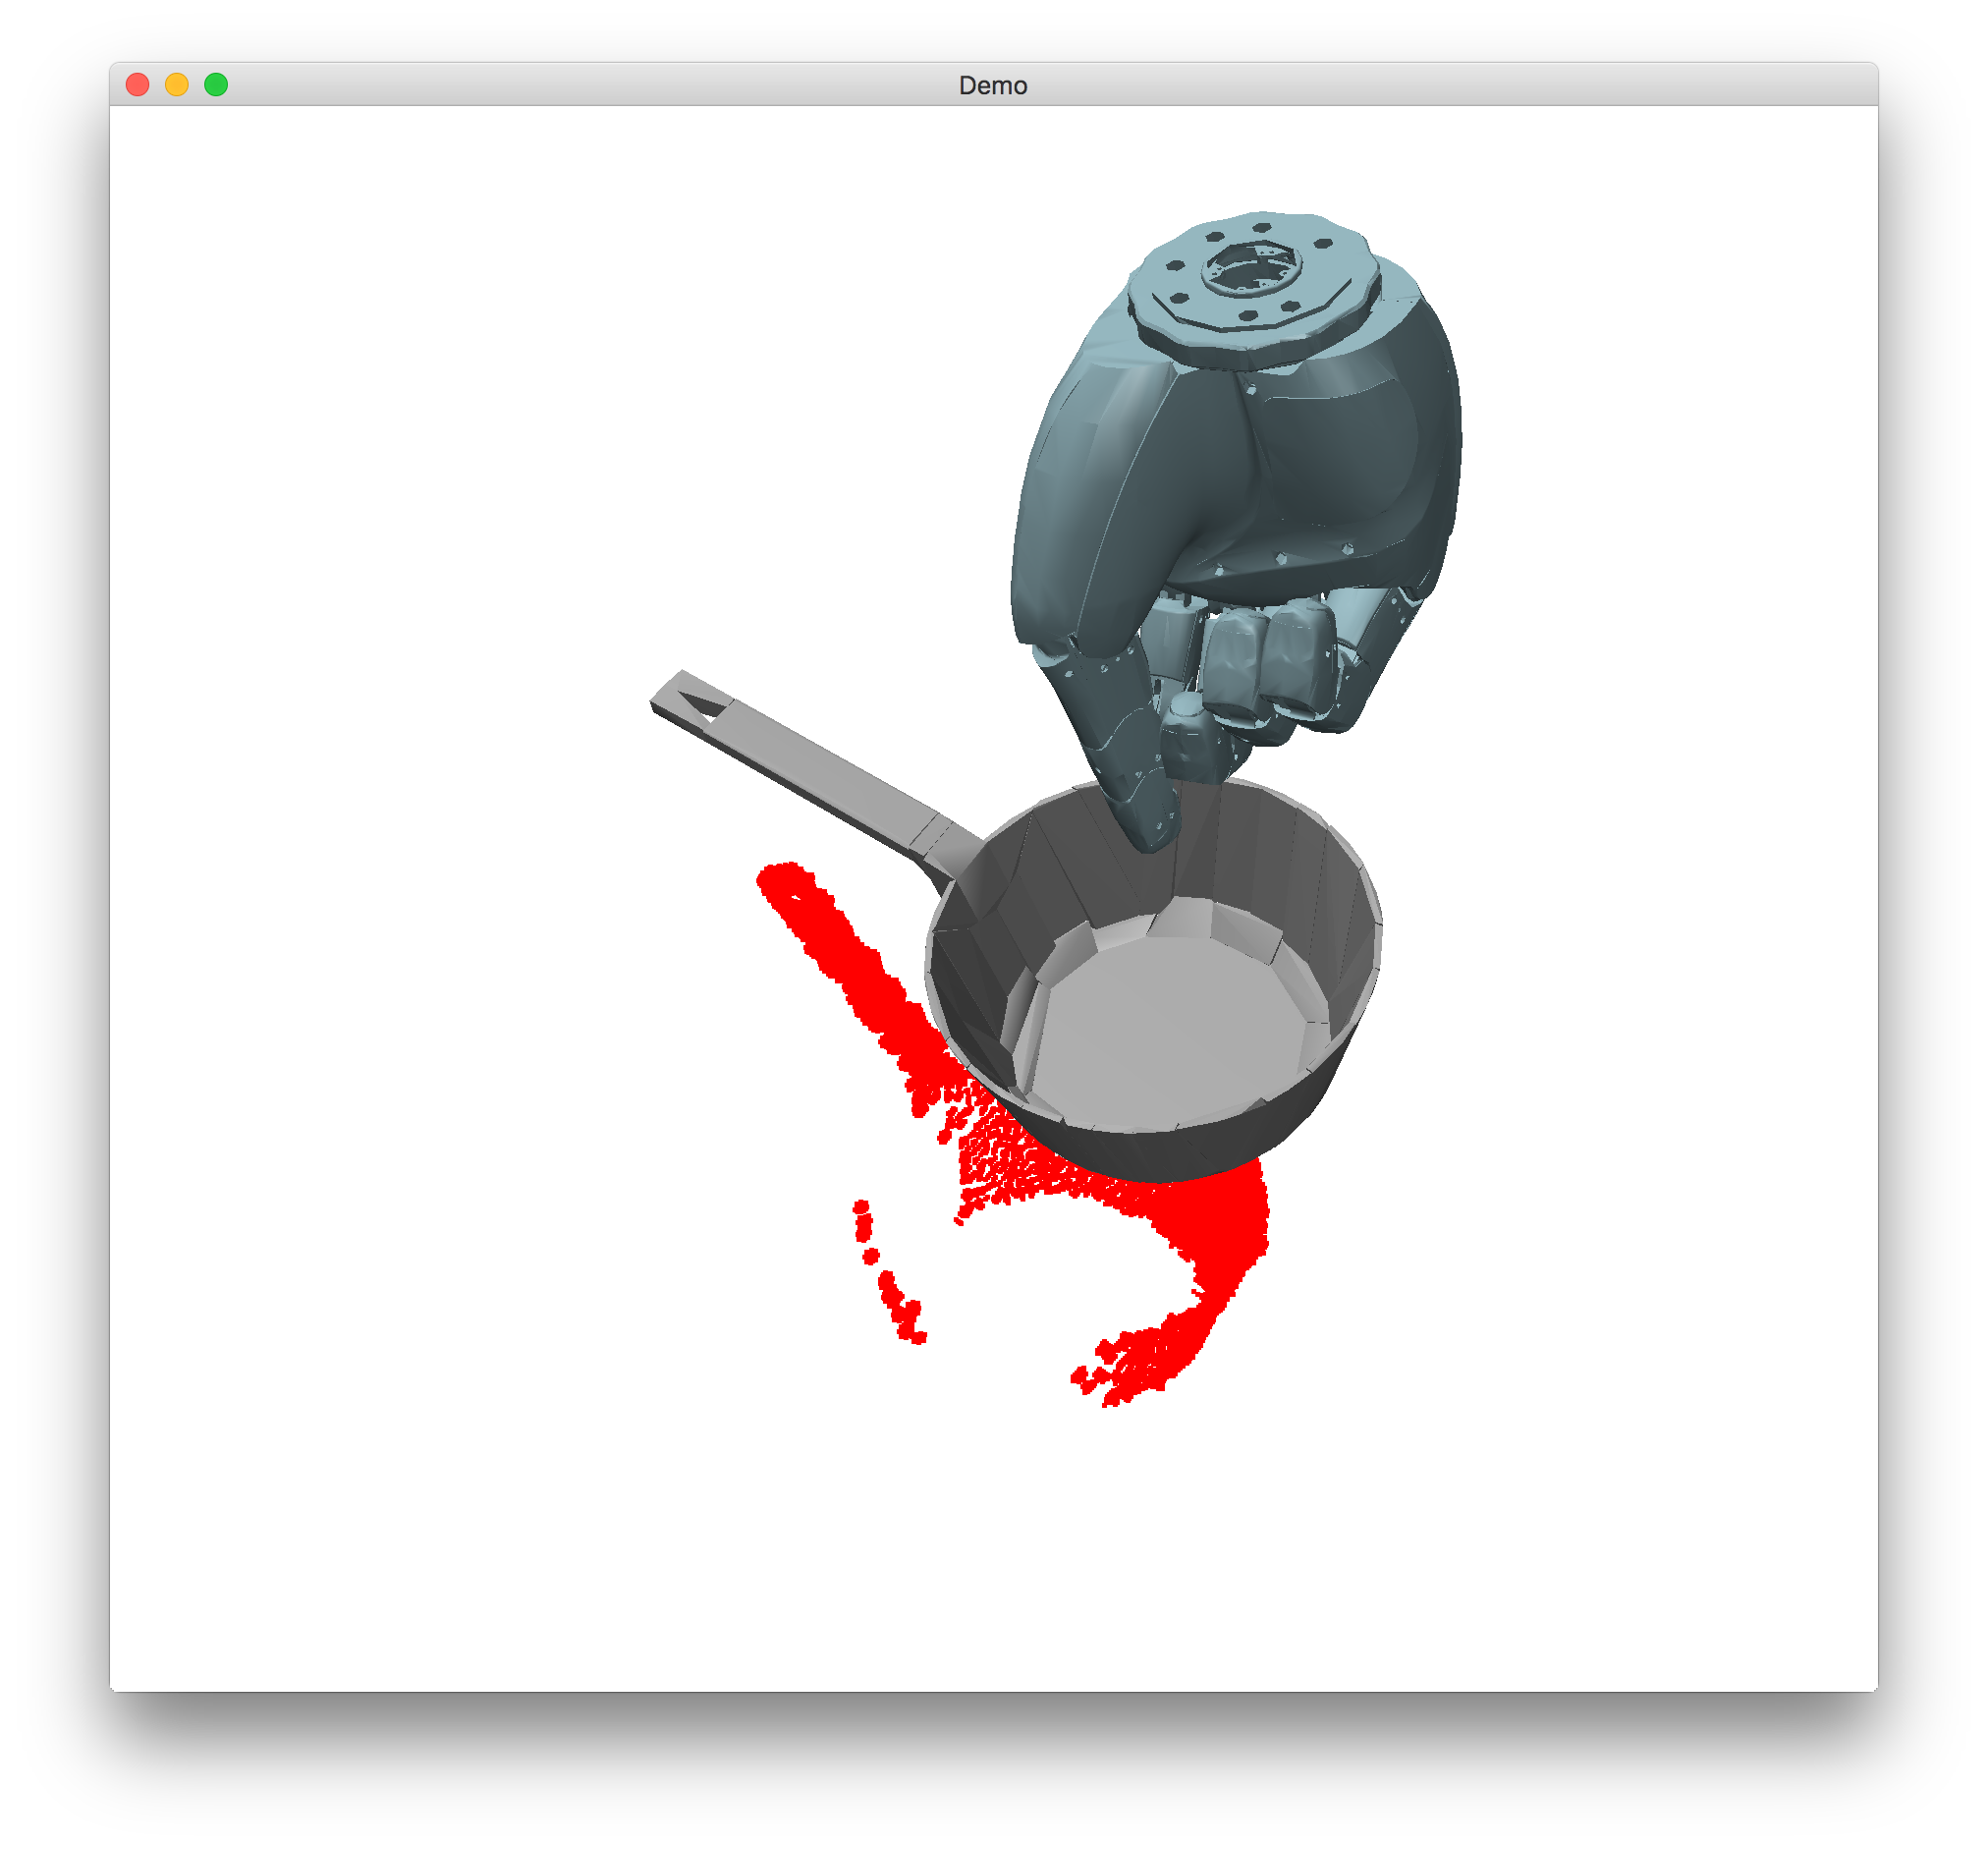
\includegraphics[width=0.24\textwidth]{images/Pan4_2_HFLW}
%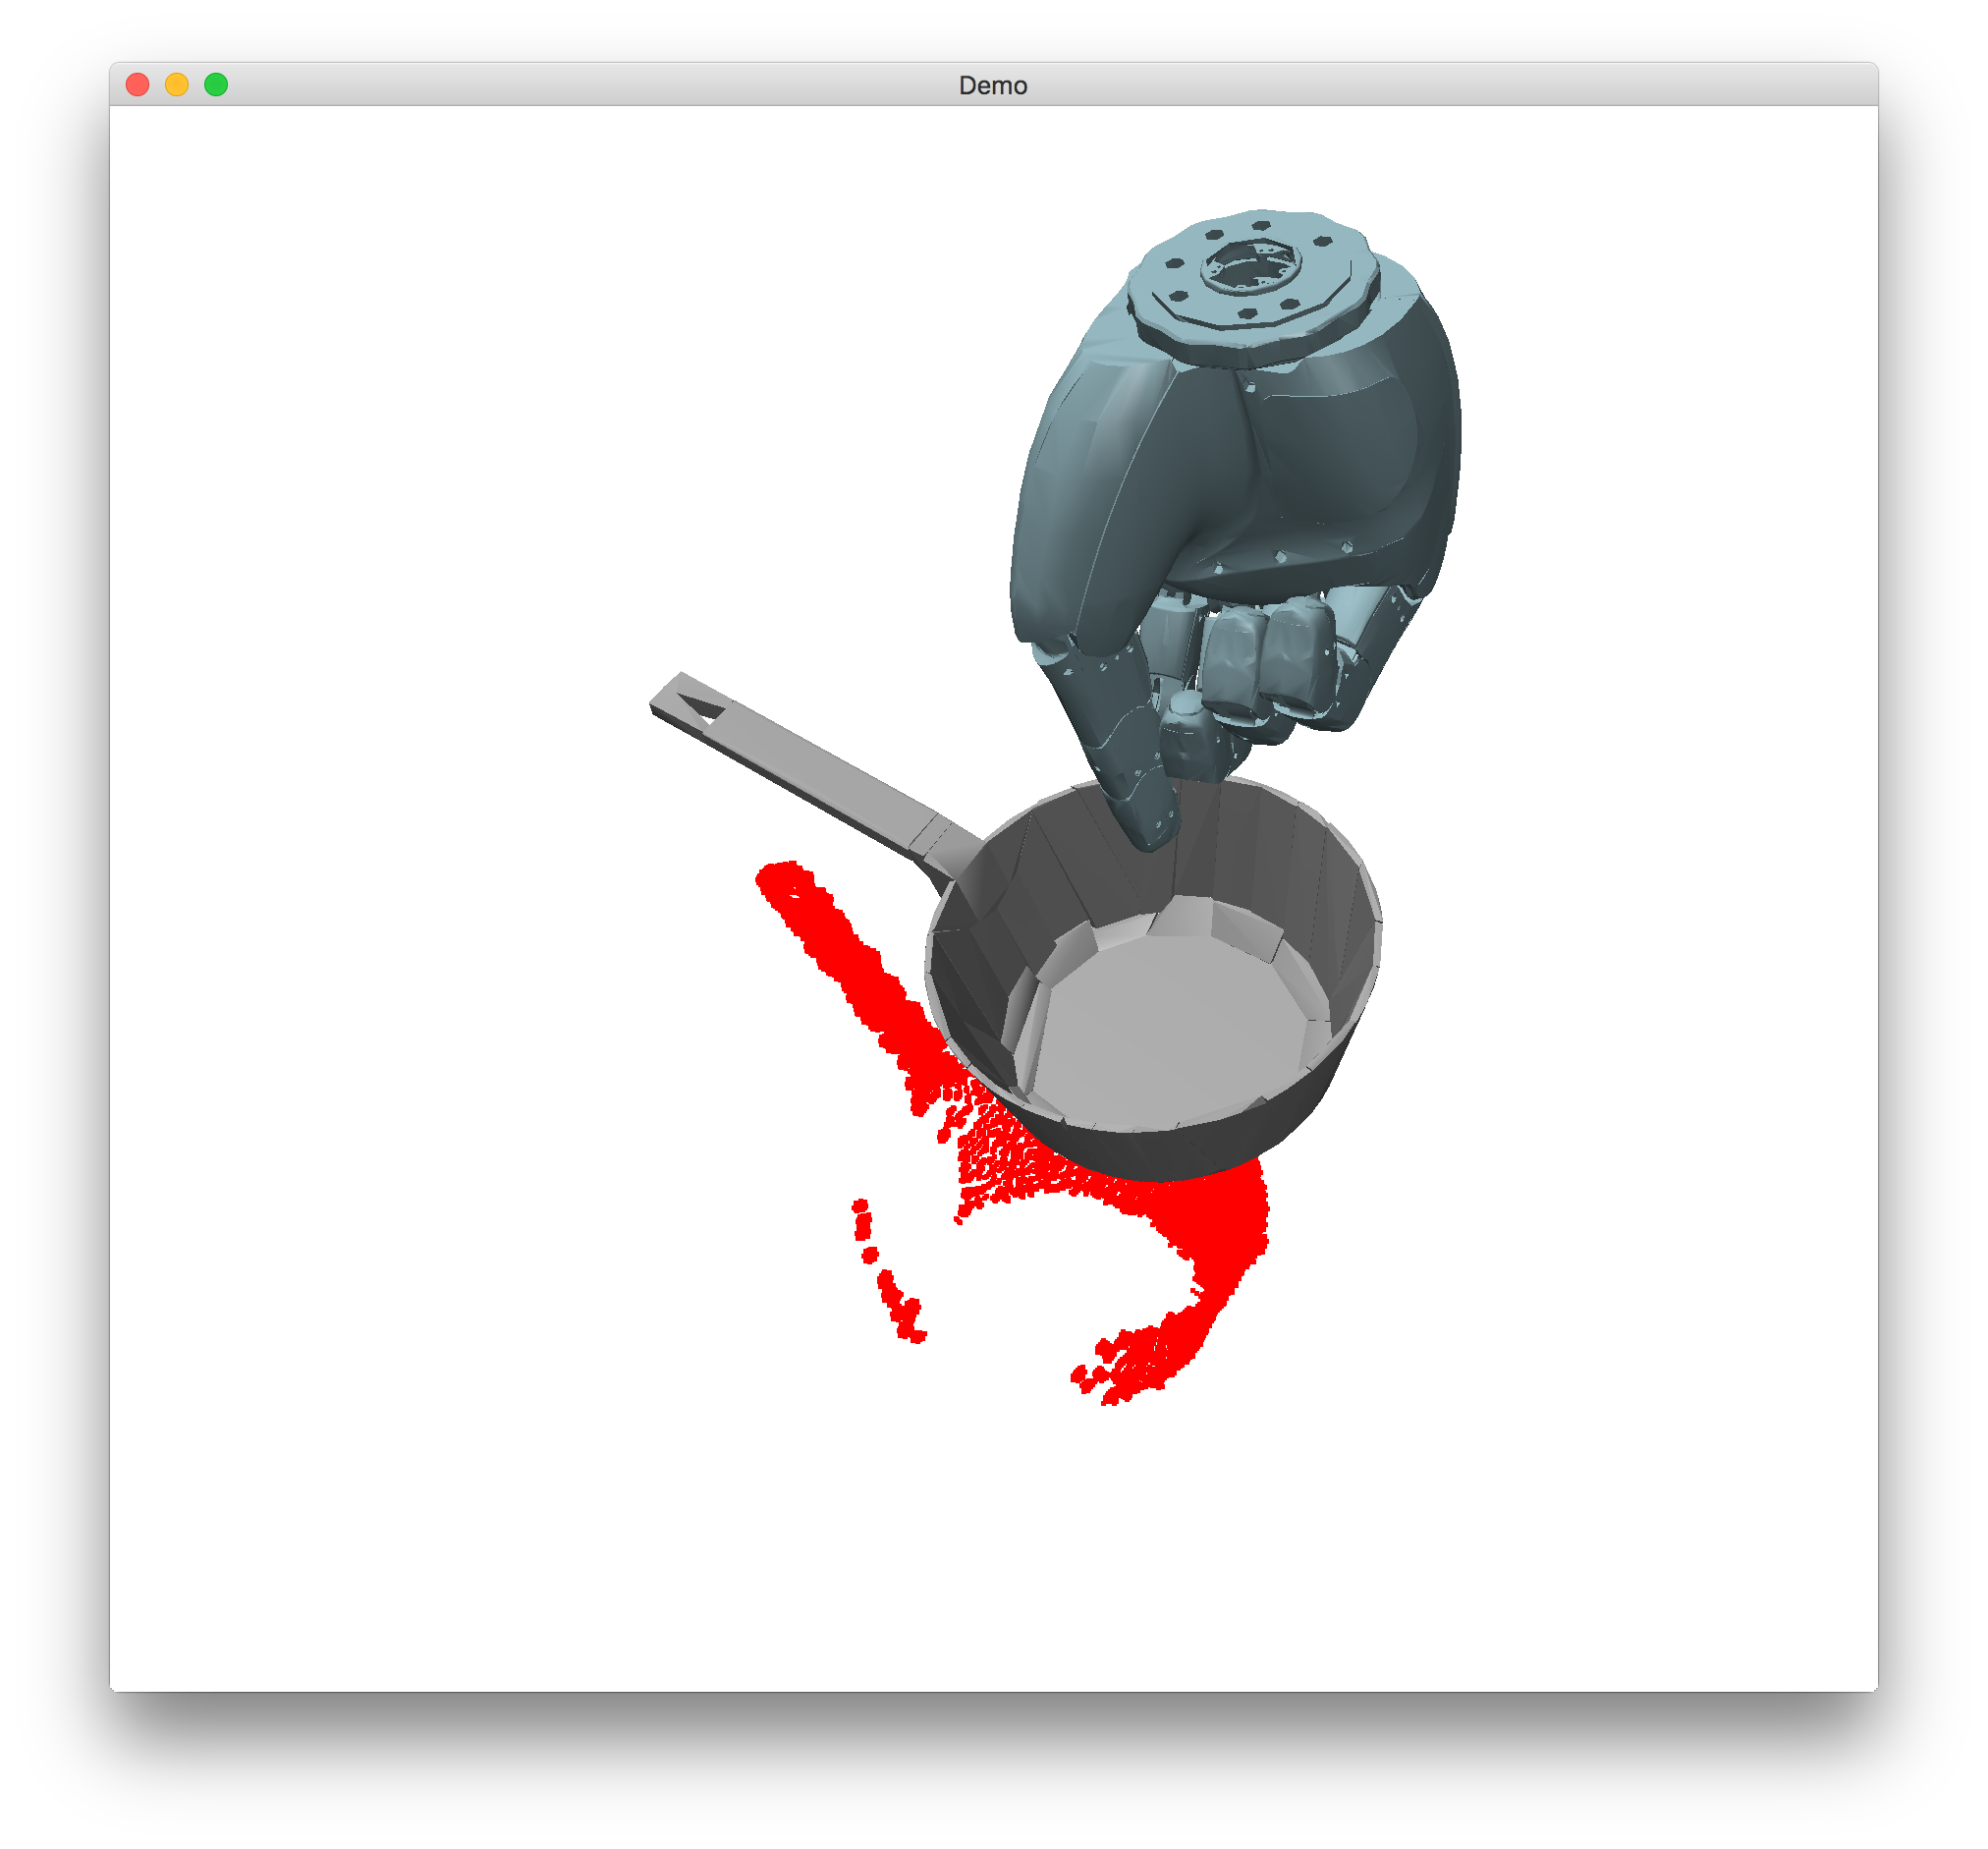
\includegraphics[width=0.24\textwidth]{images/Pan4_2_LFLW}
%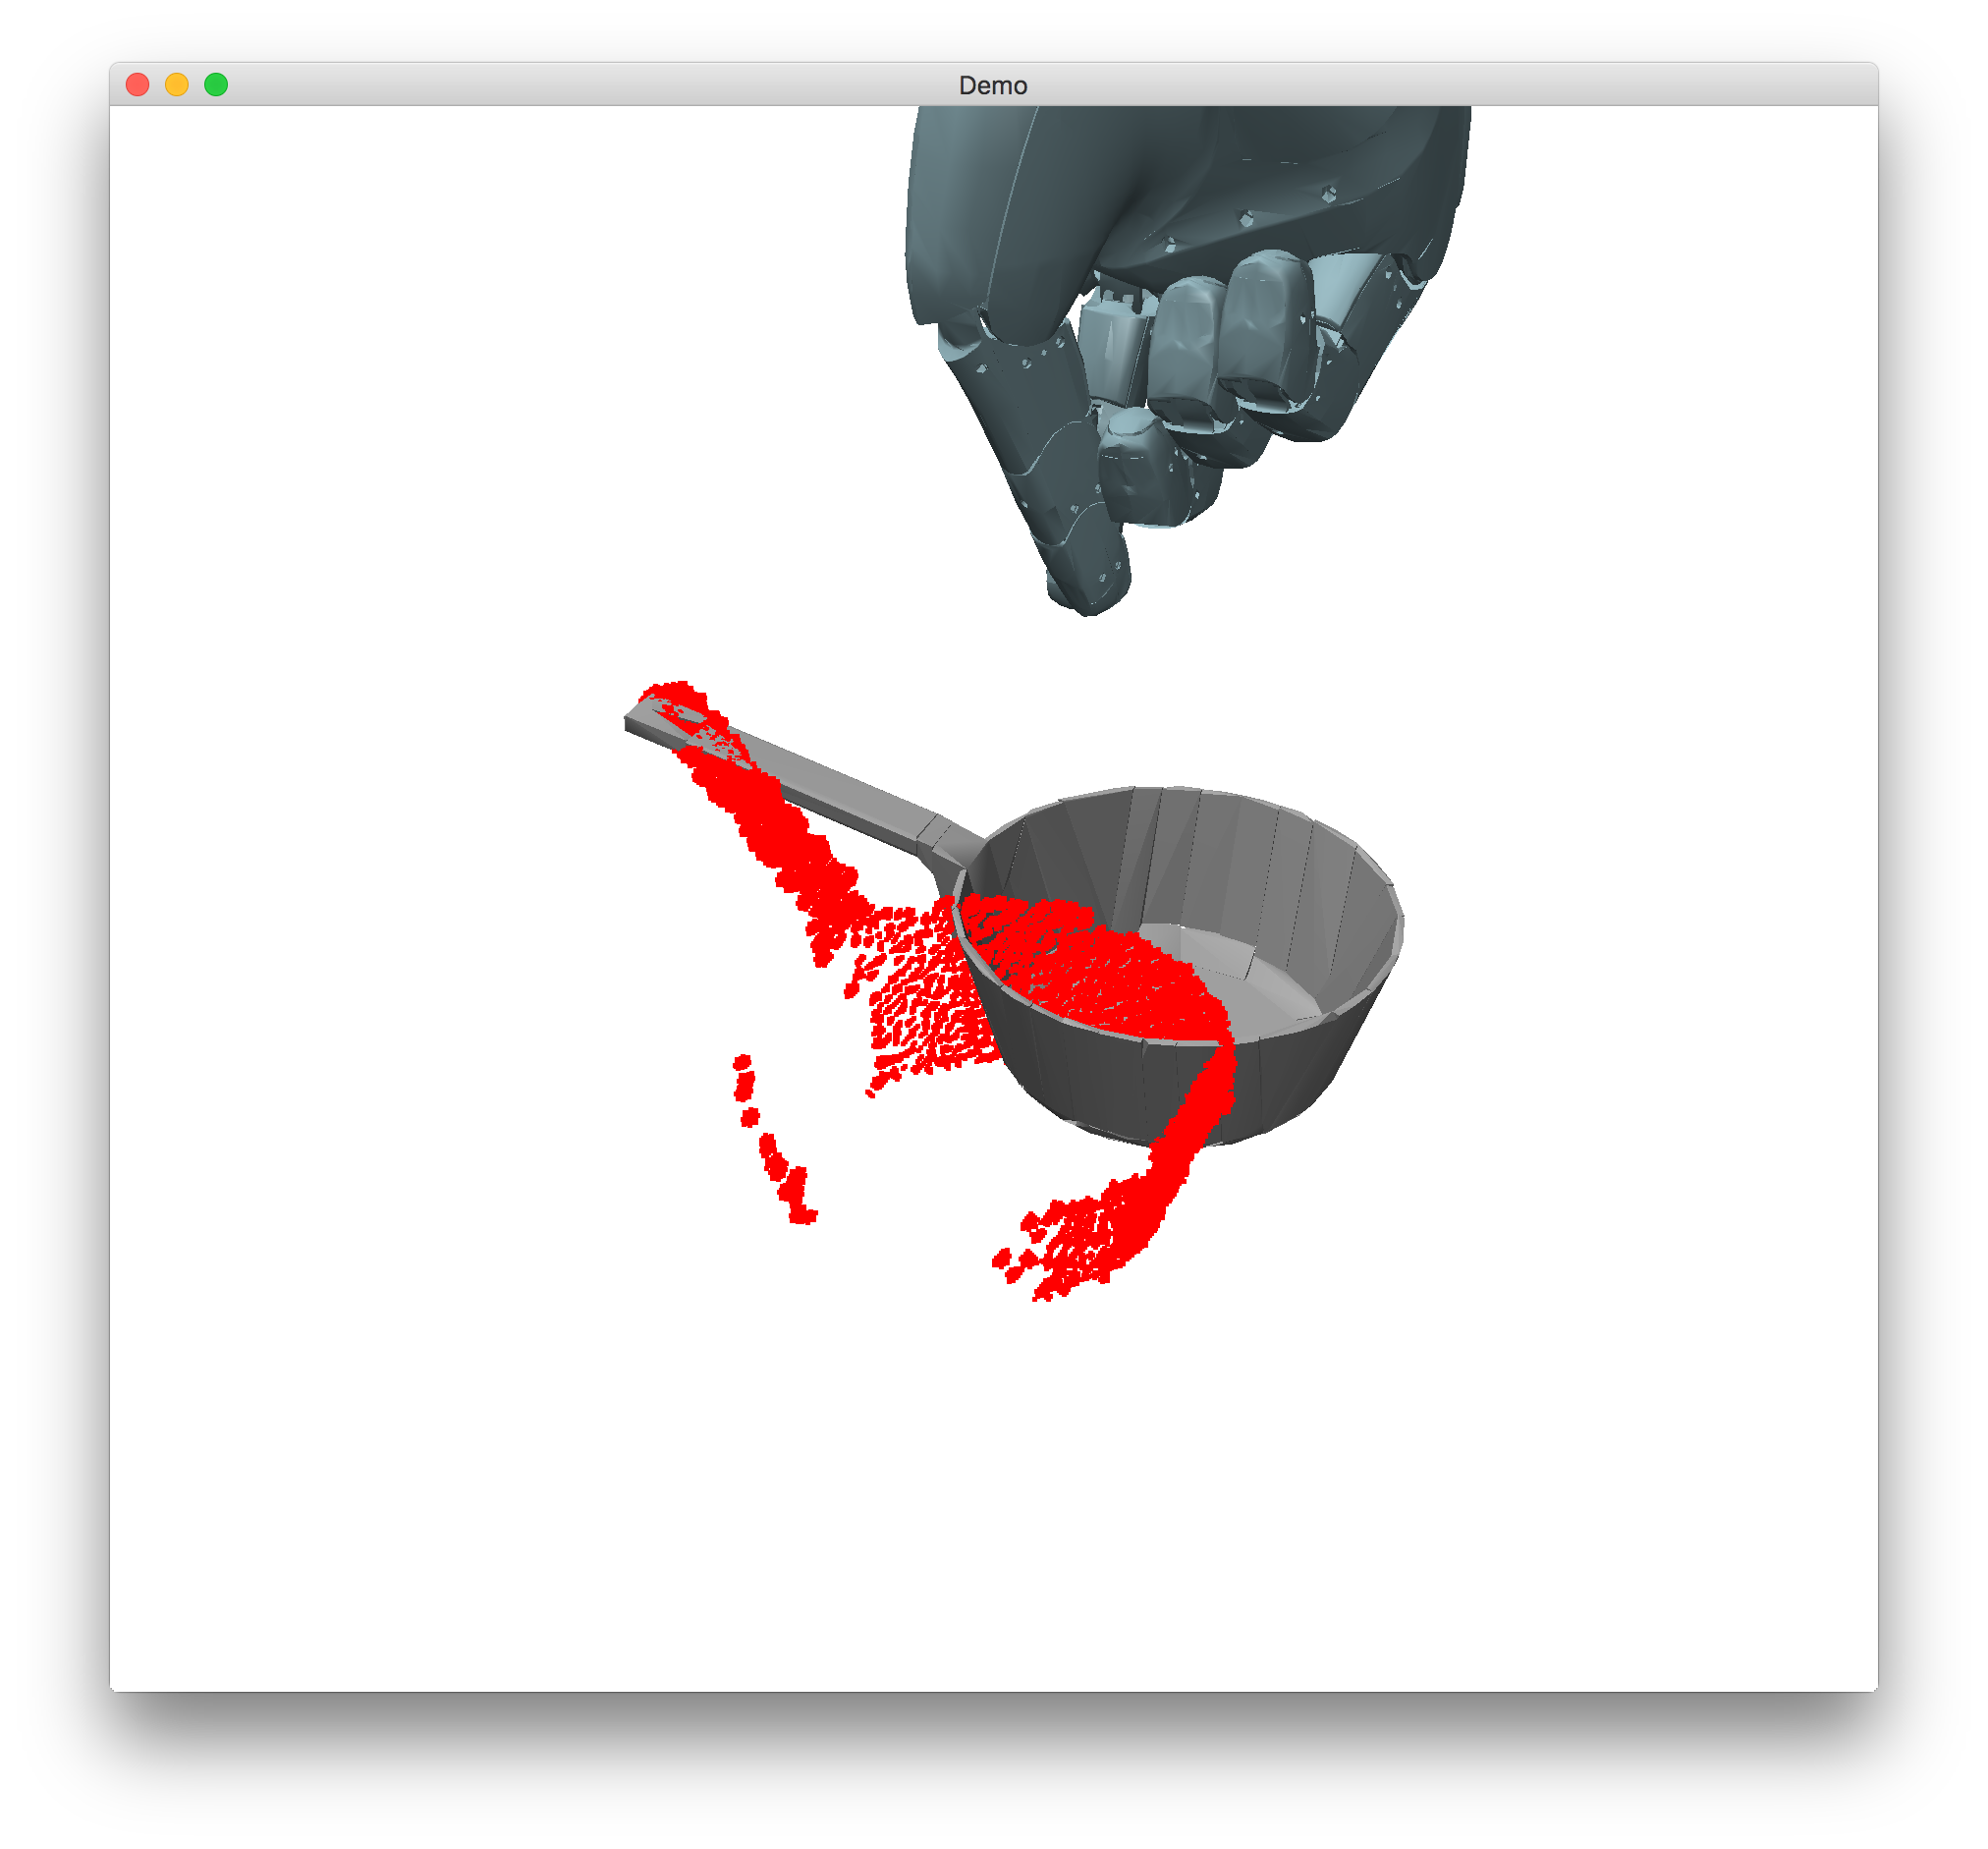
\includegraphics[width=0.24\textwidth]{images/Pan4_2_HFHW}
%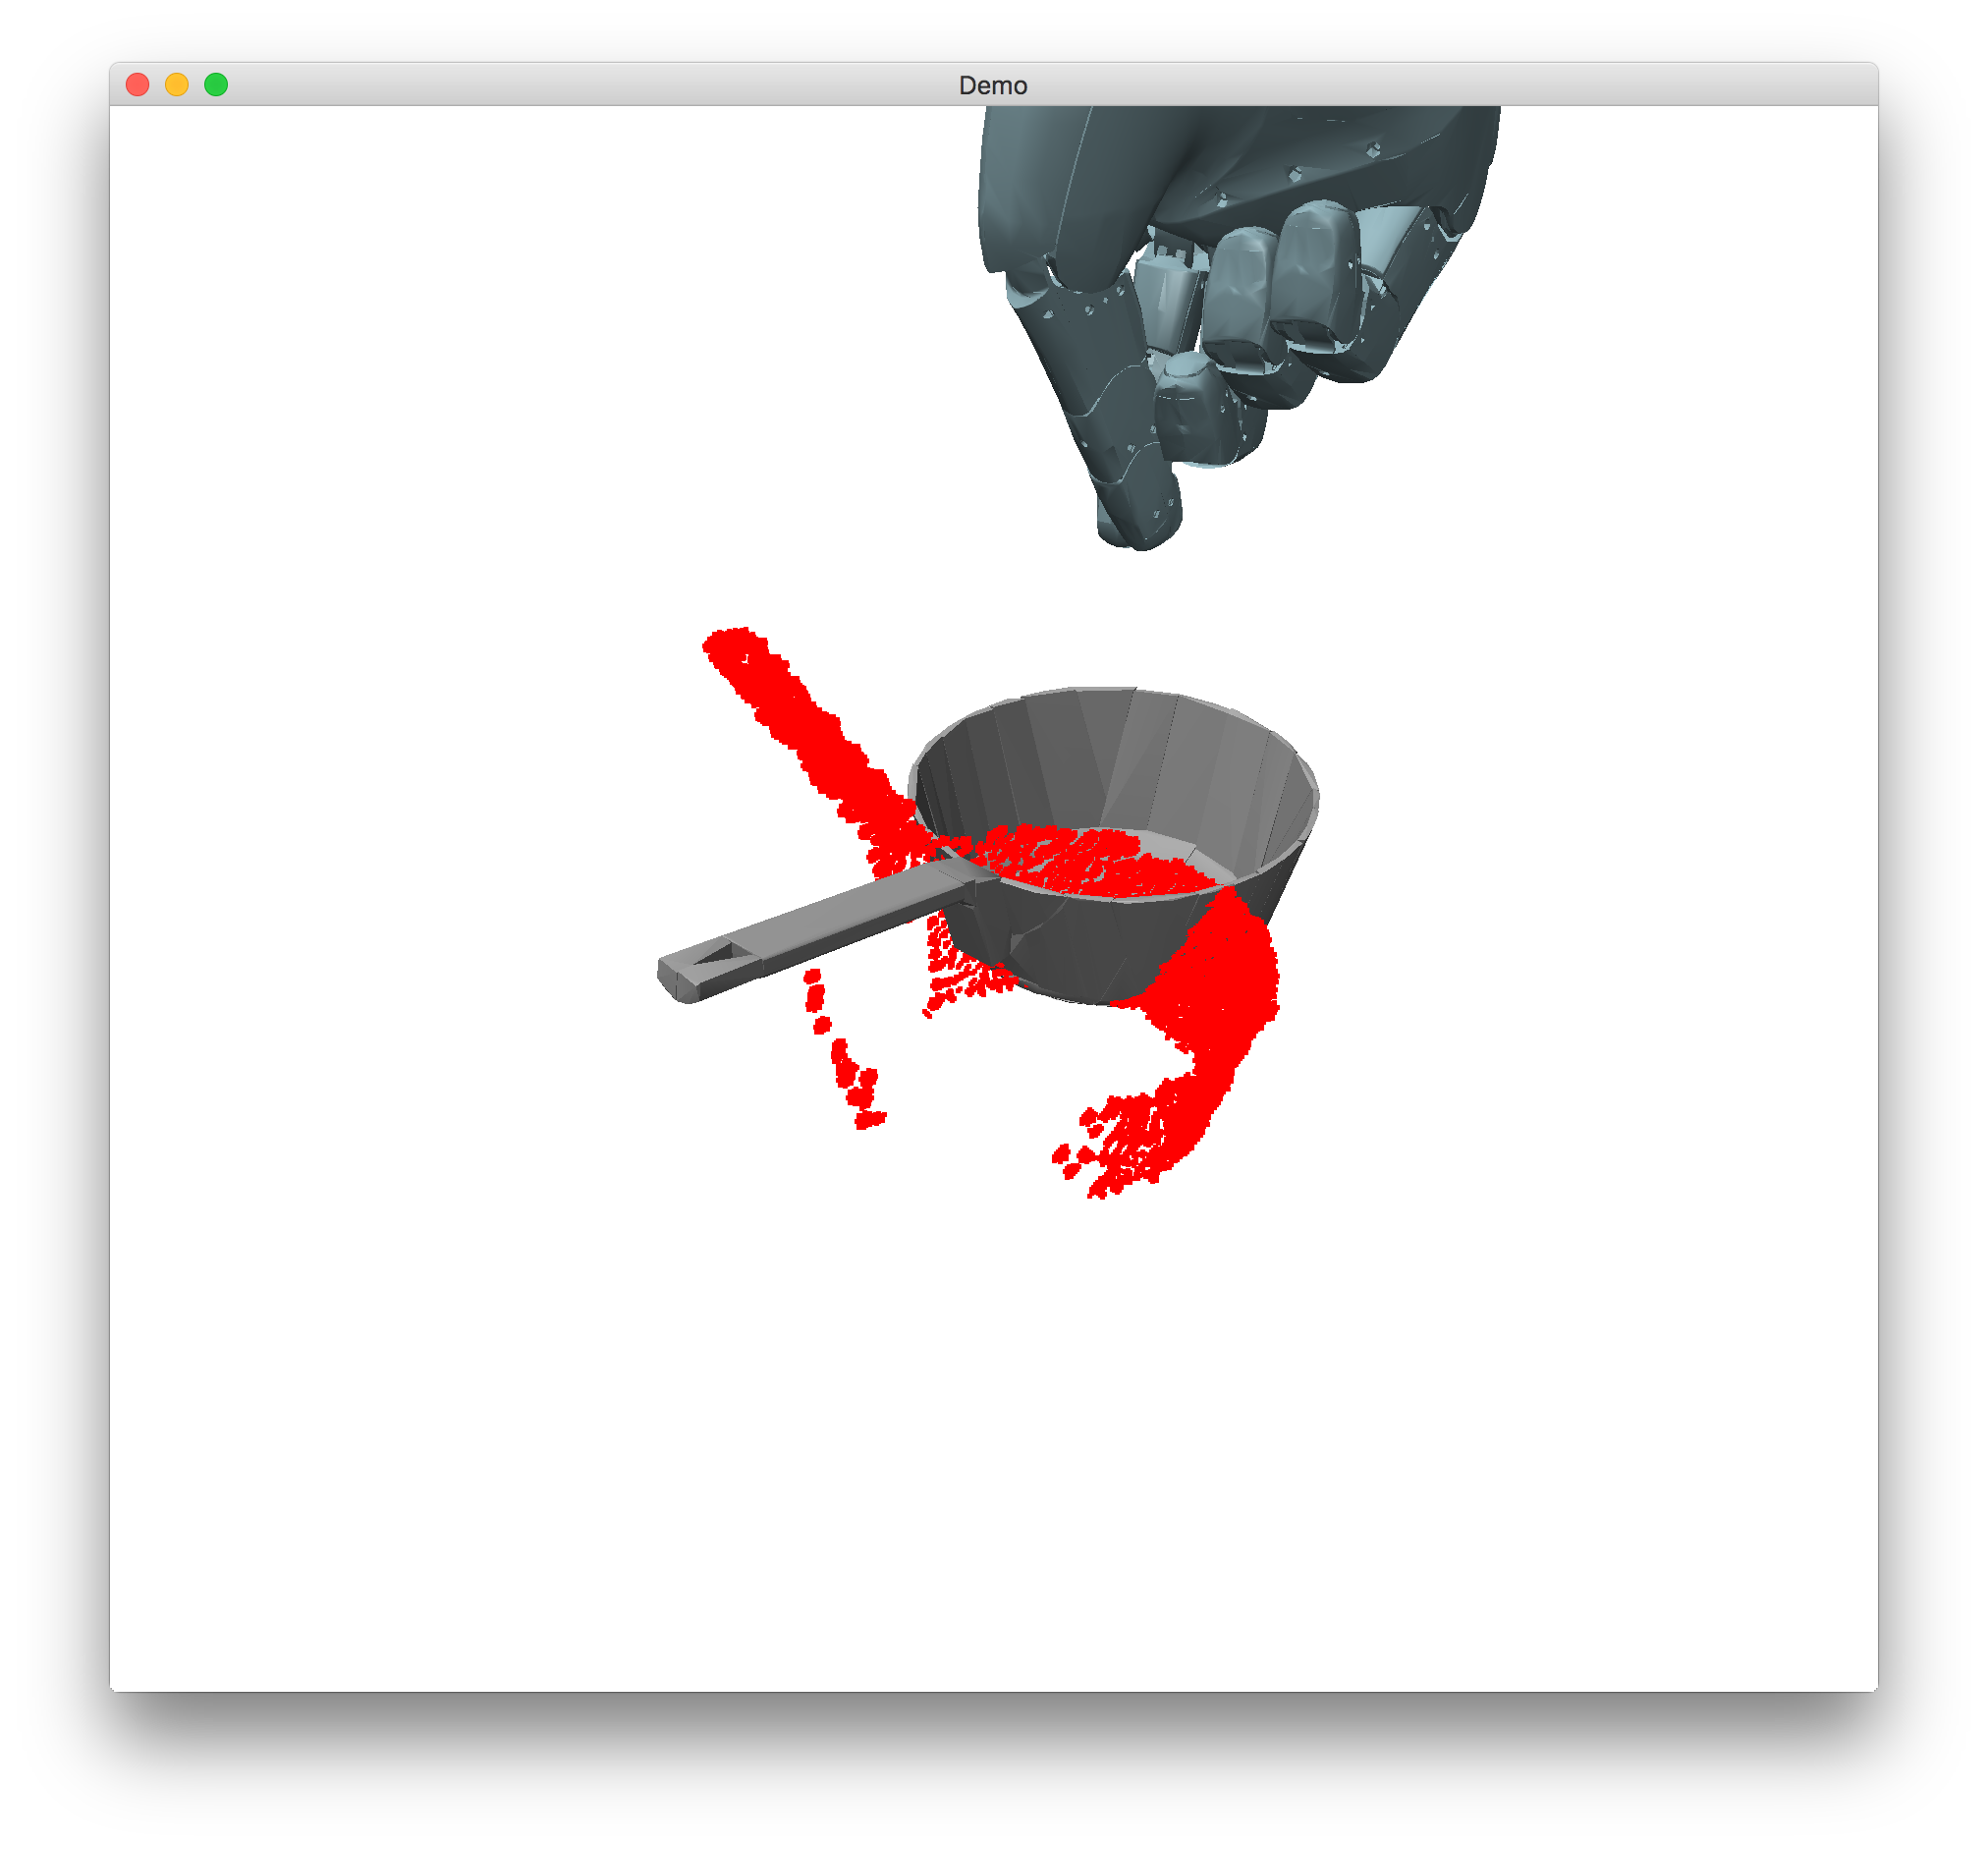
\includegraphics[width=0.24\textwidth]{images/Pan4_2_LFHW}\\
%%
\includegraphics[width=0.96\textwidth]{images/key-to-eval-training}\\
%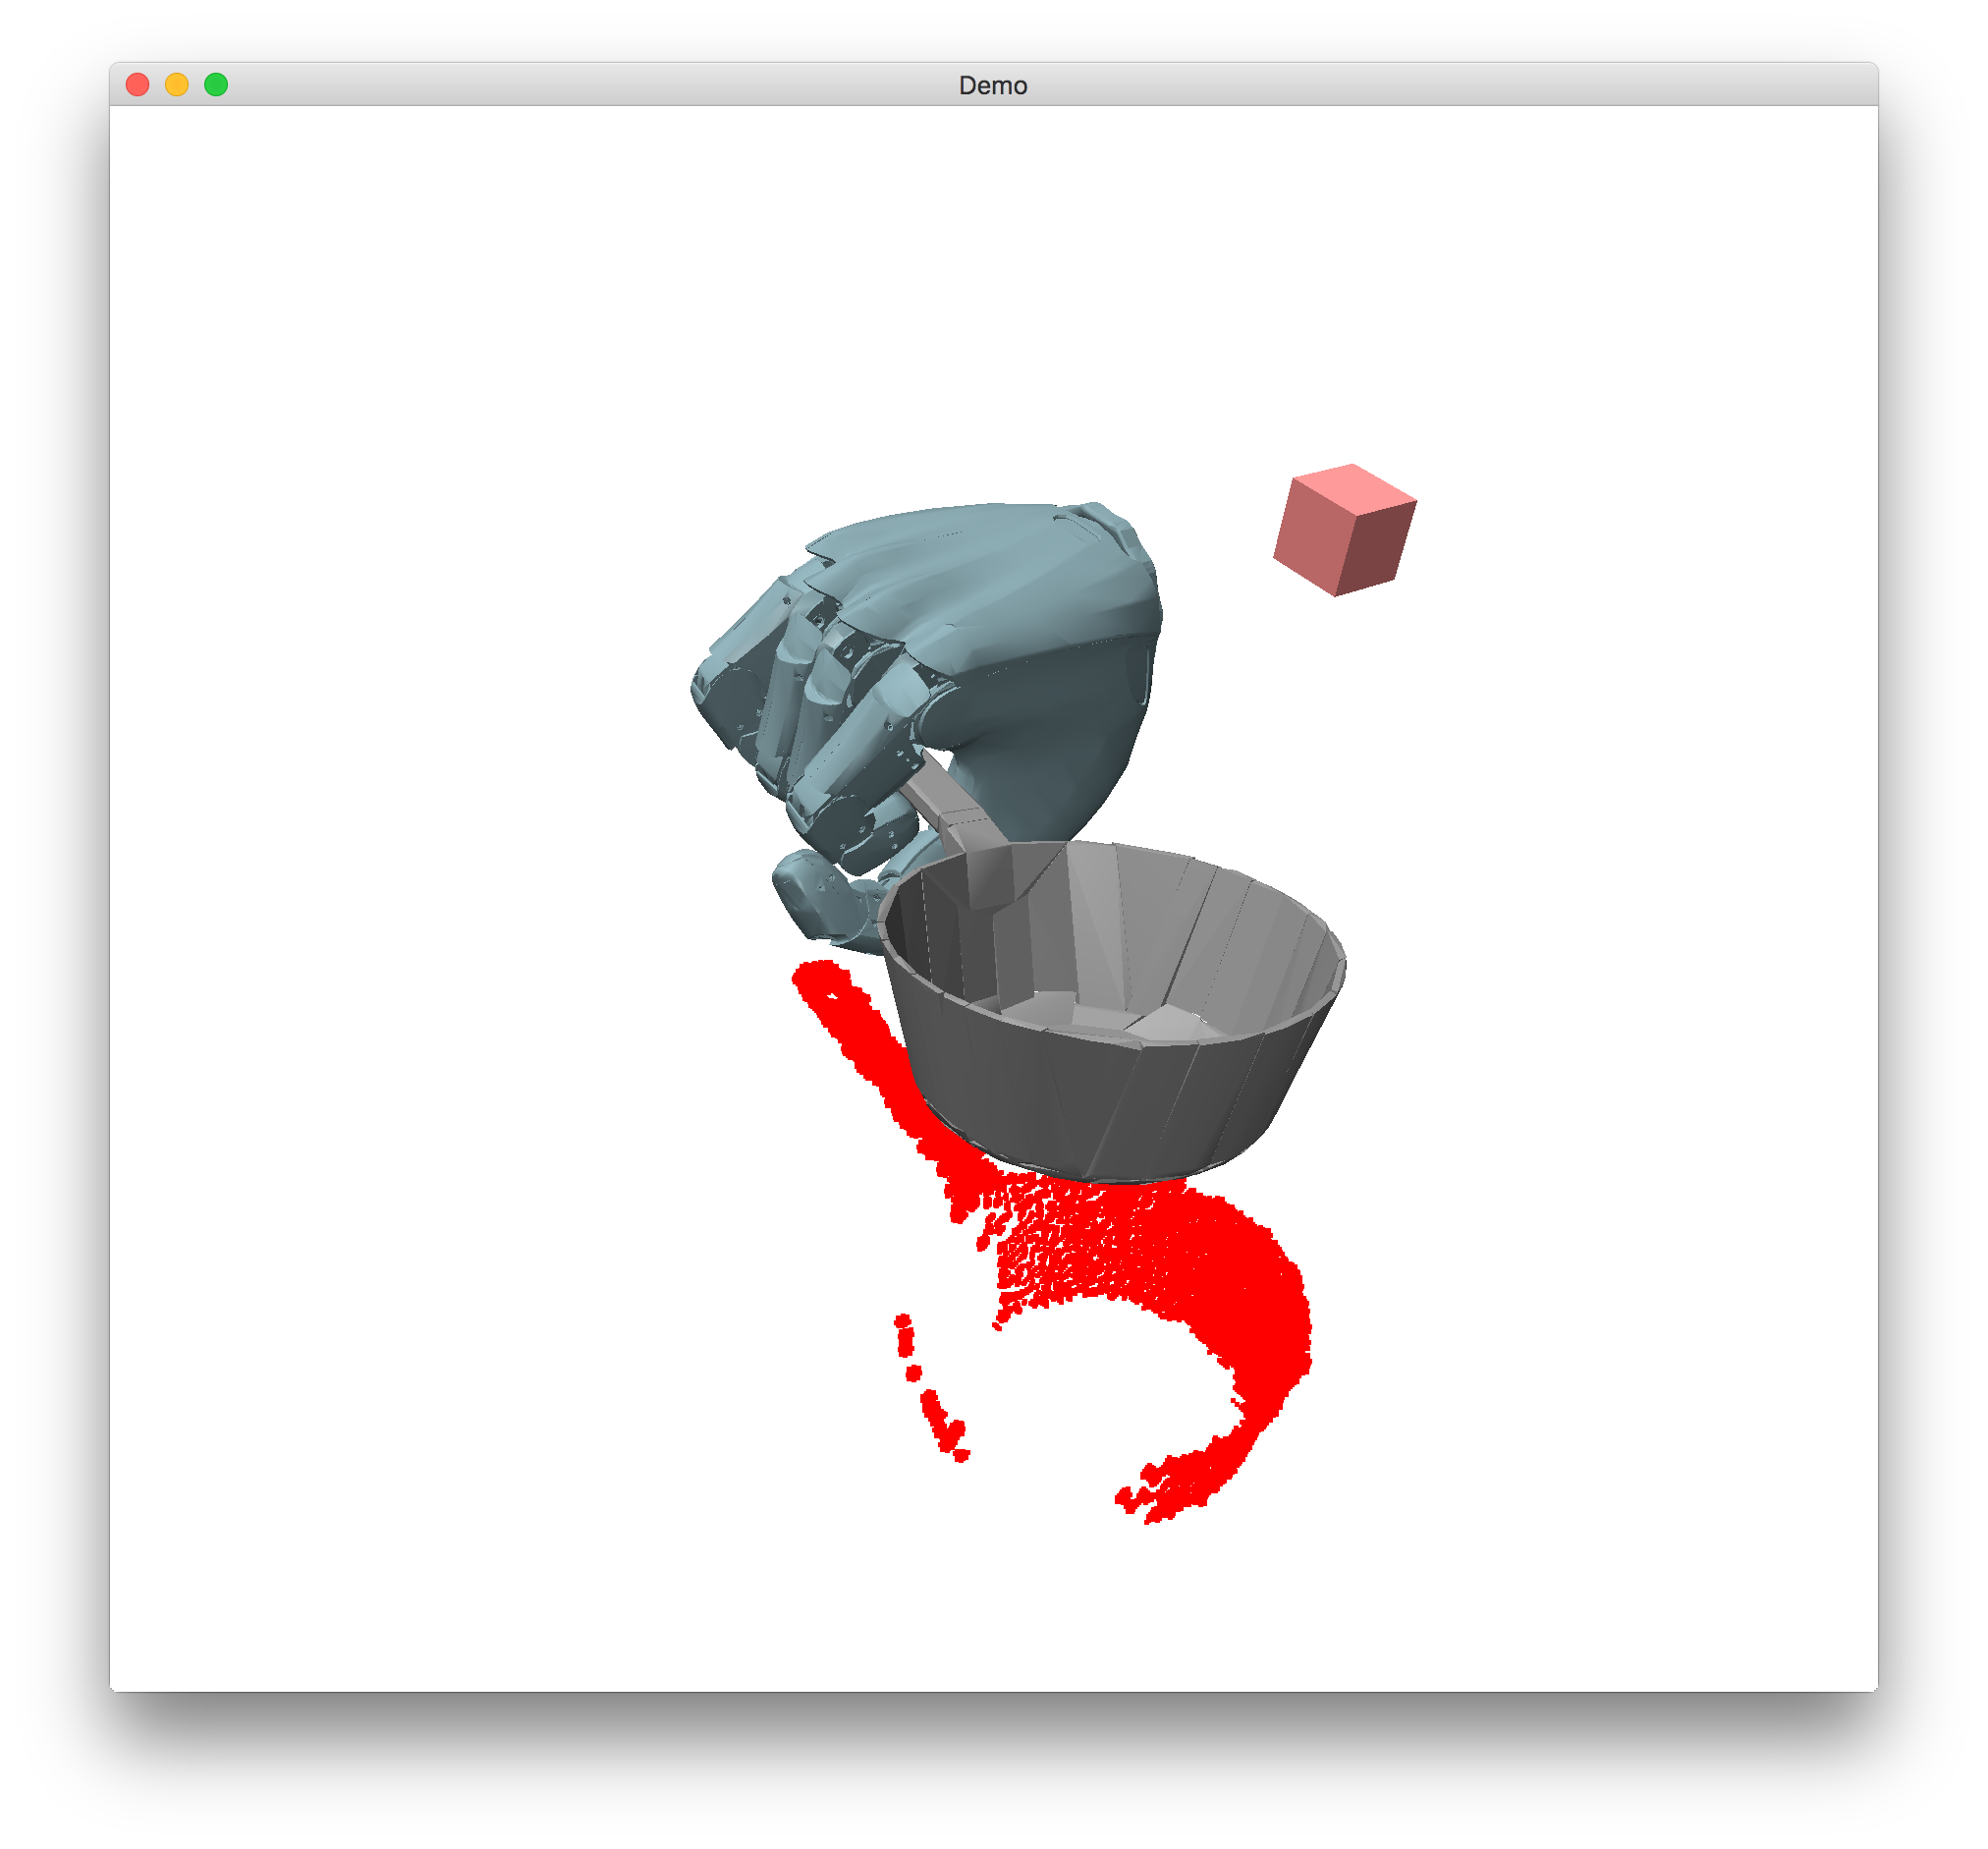
\includegraphics[width=0.24\textwidth]{images/Pan4_HFLW}
%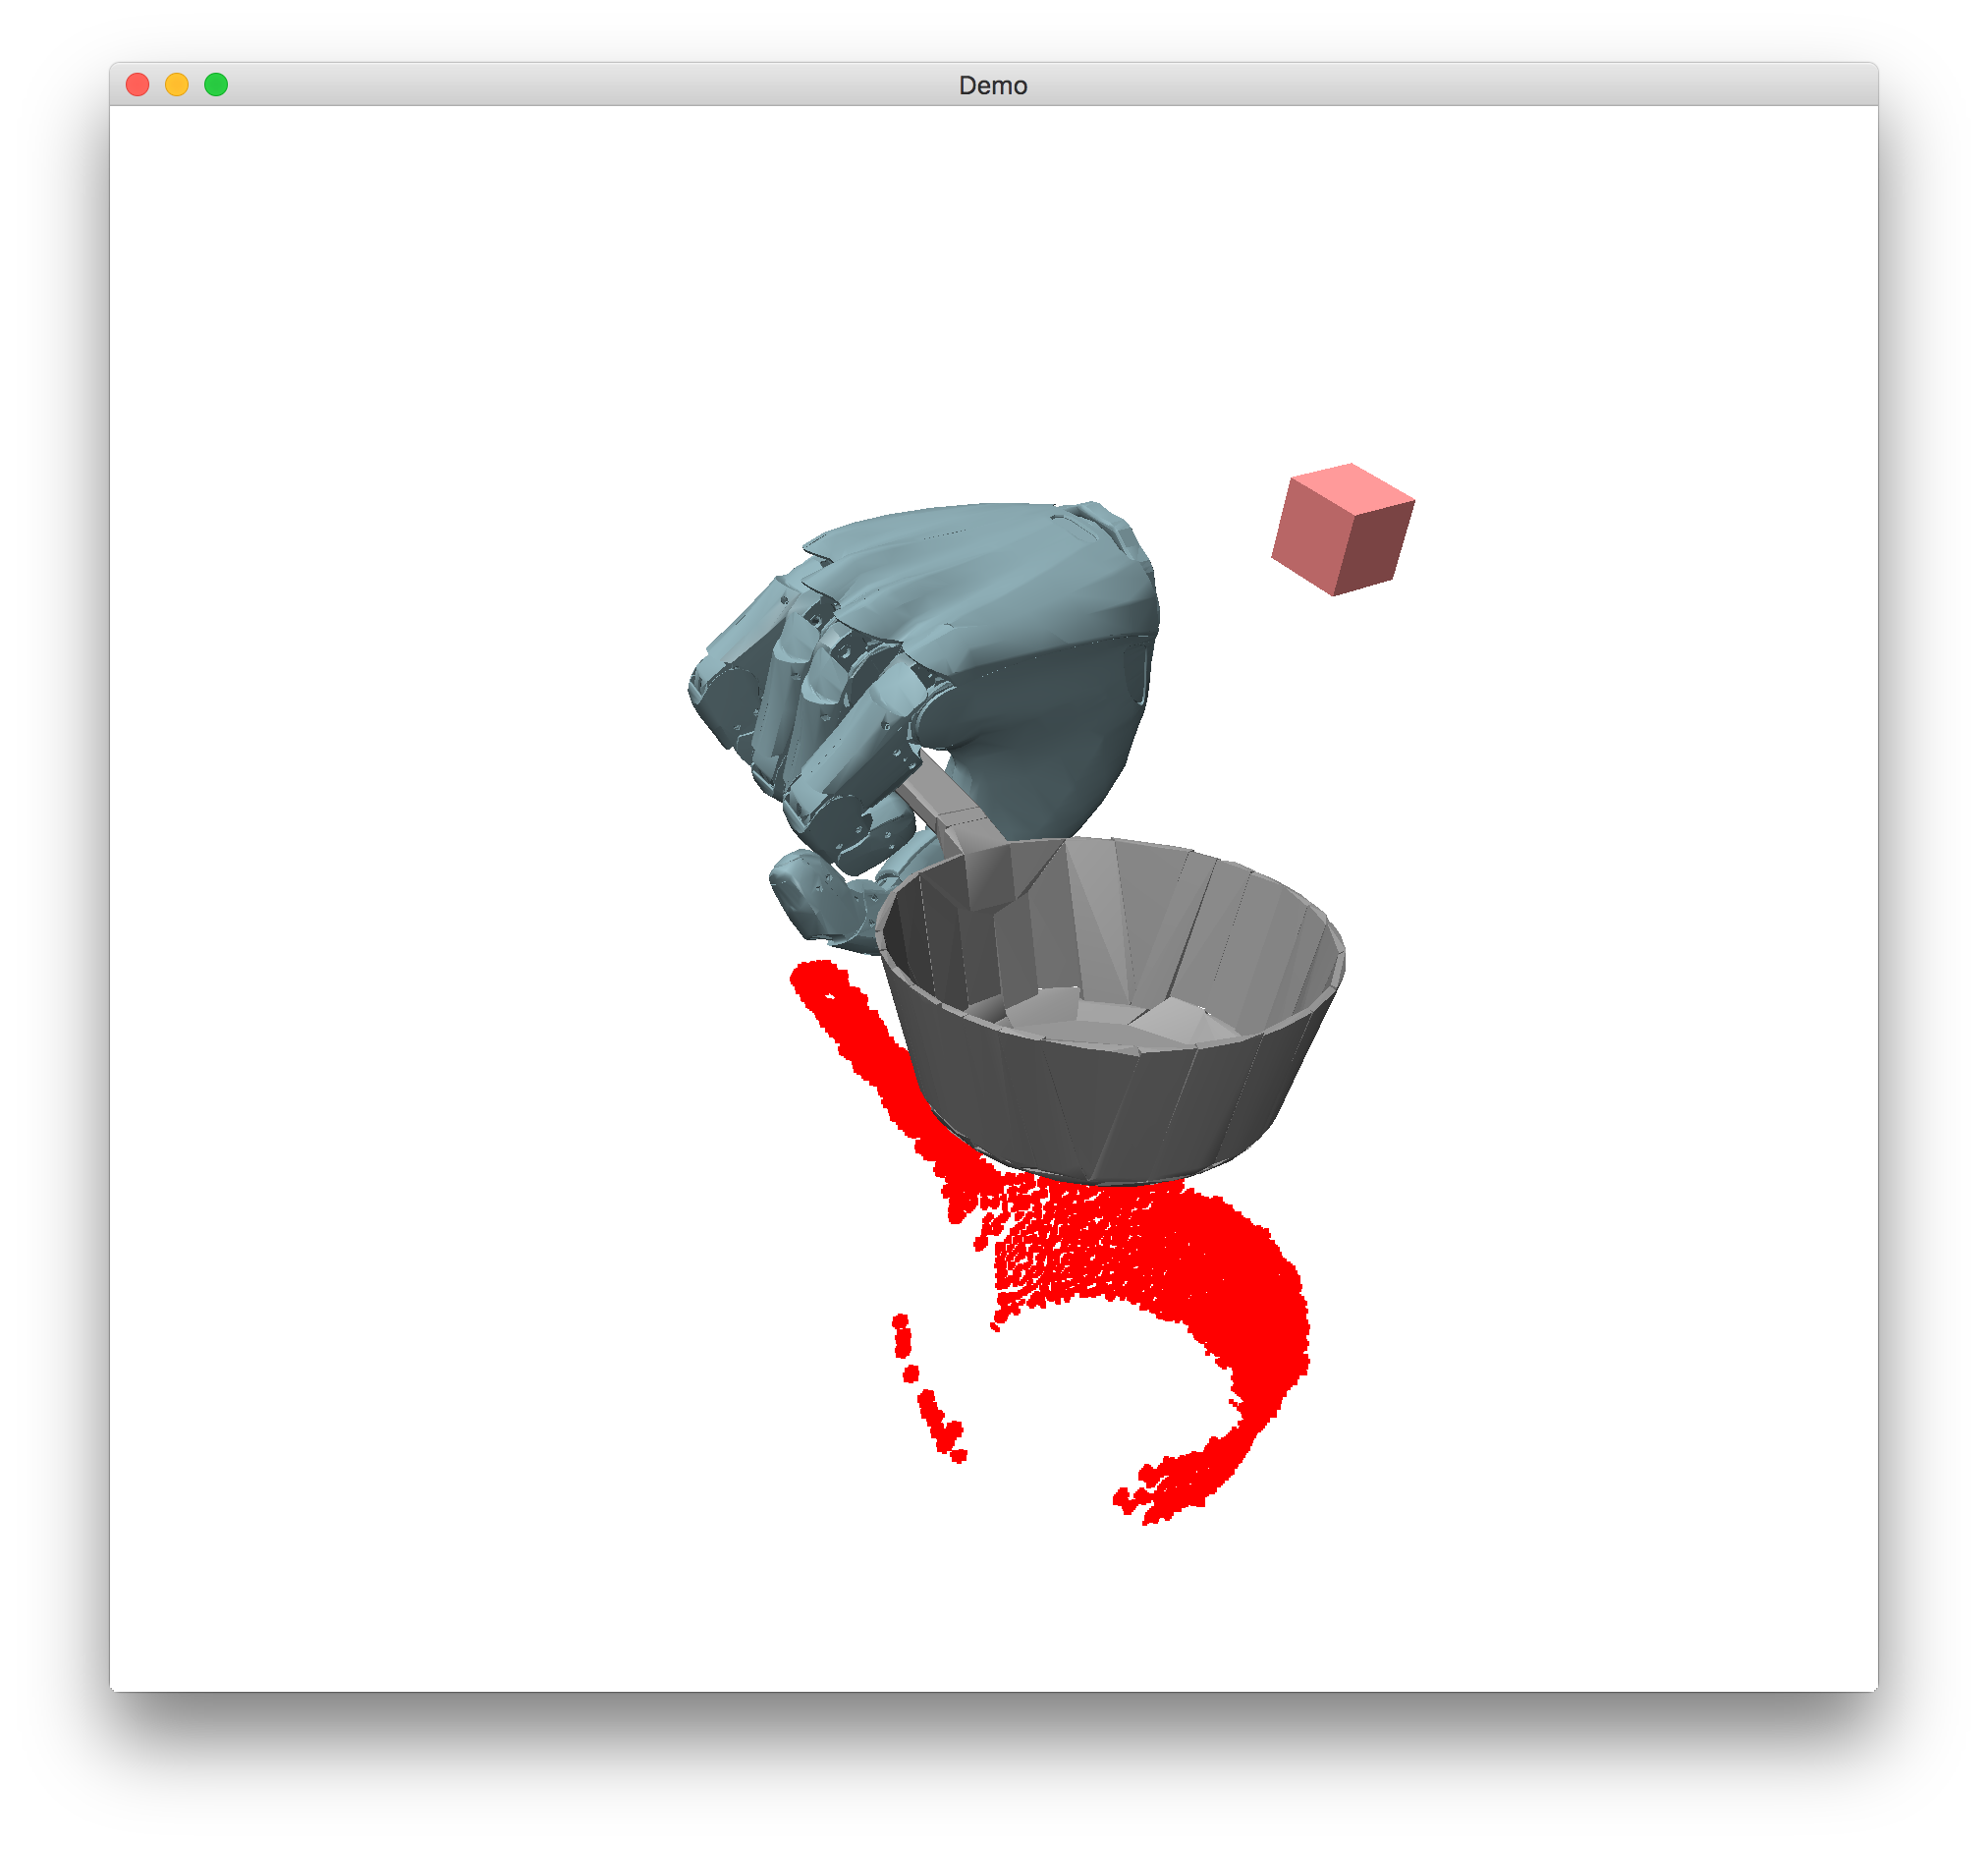
\includegraphics[width=0.24\textwidth]{images/Pan4_LFLW}
%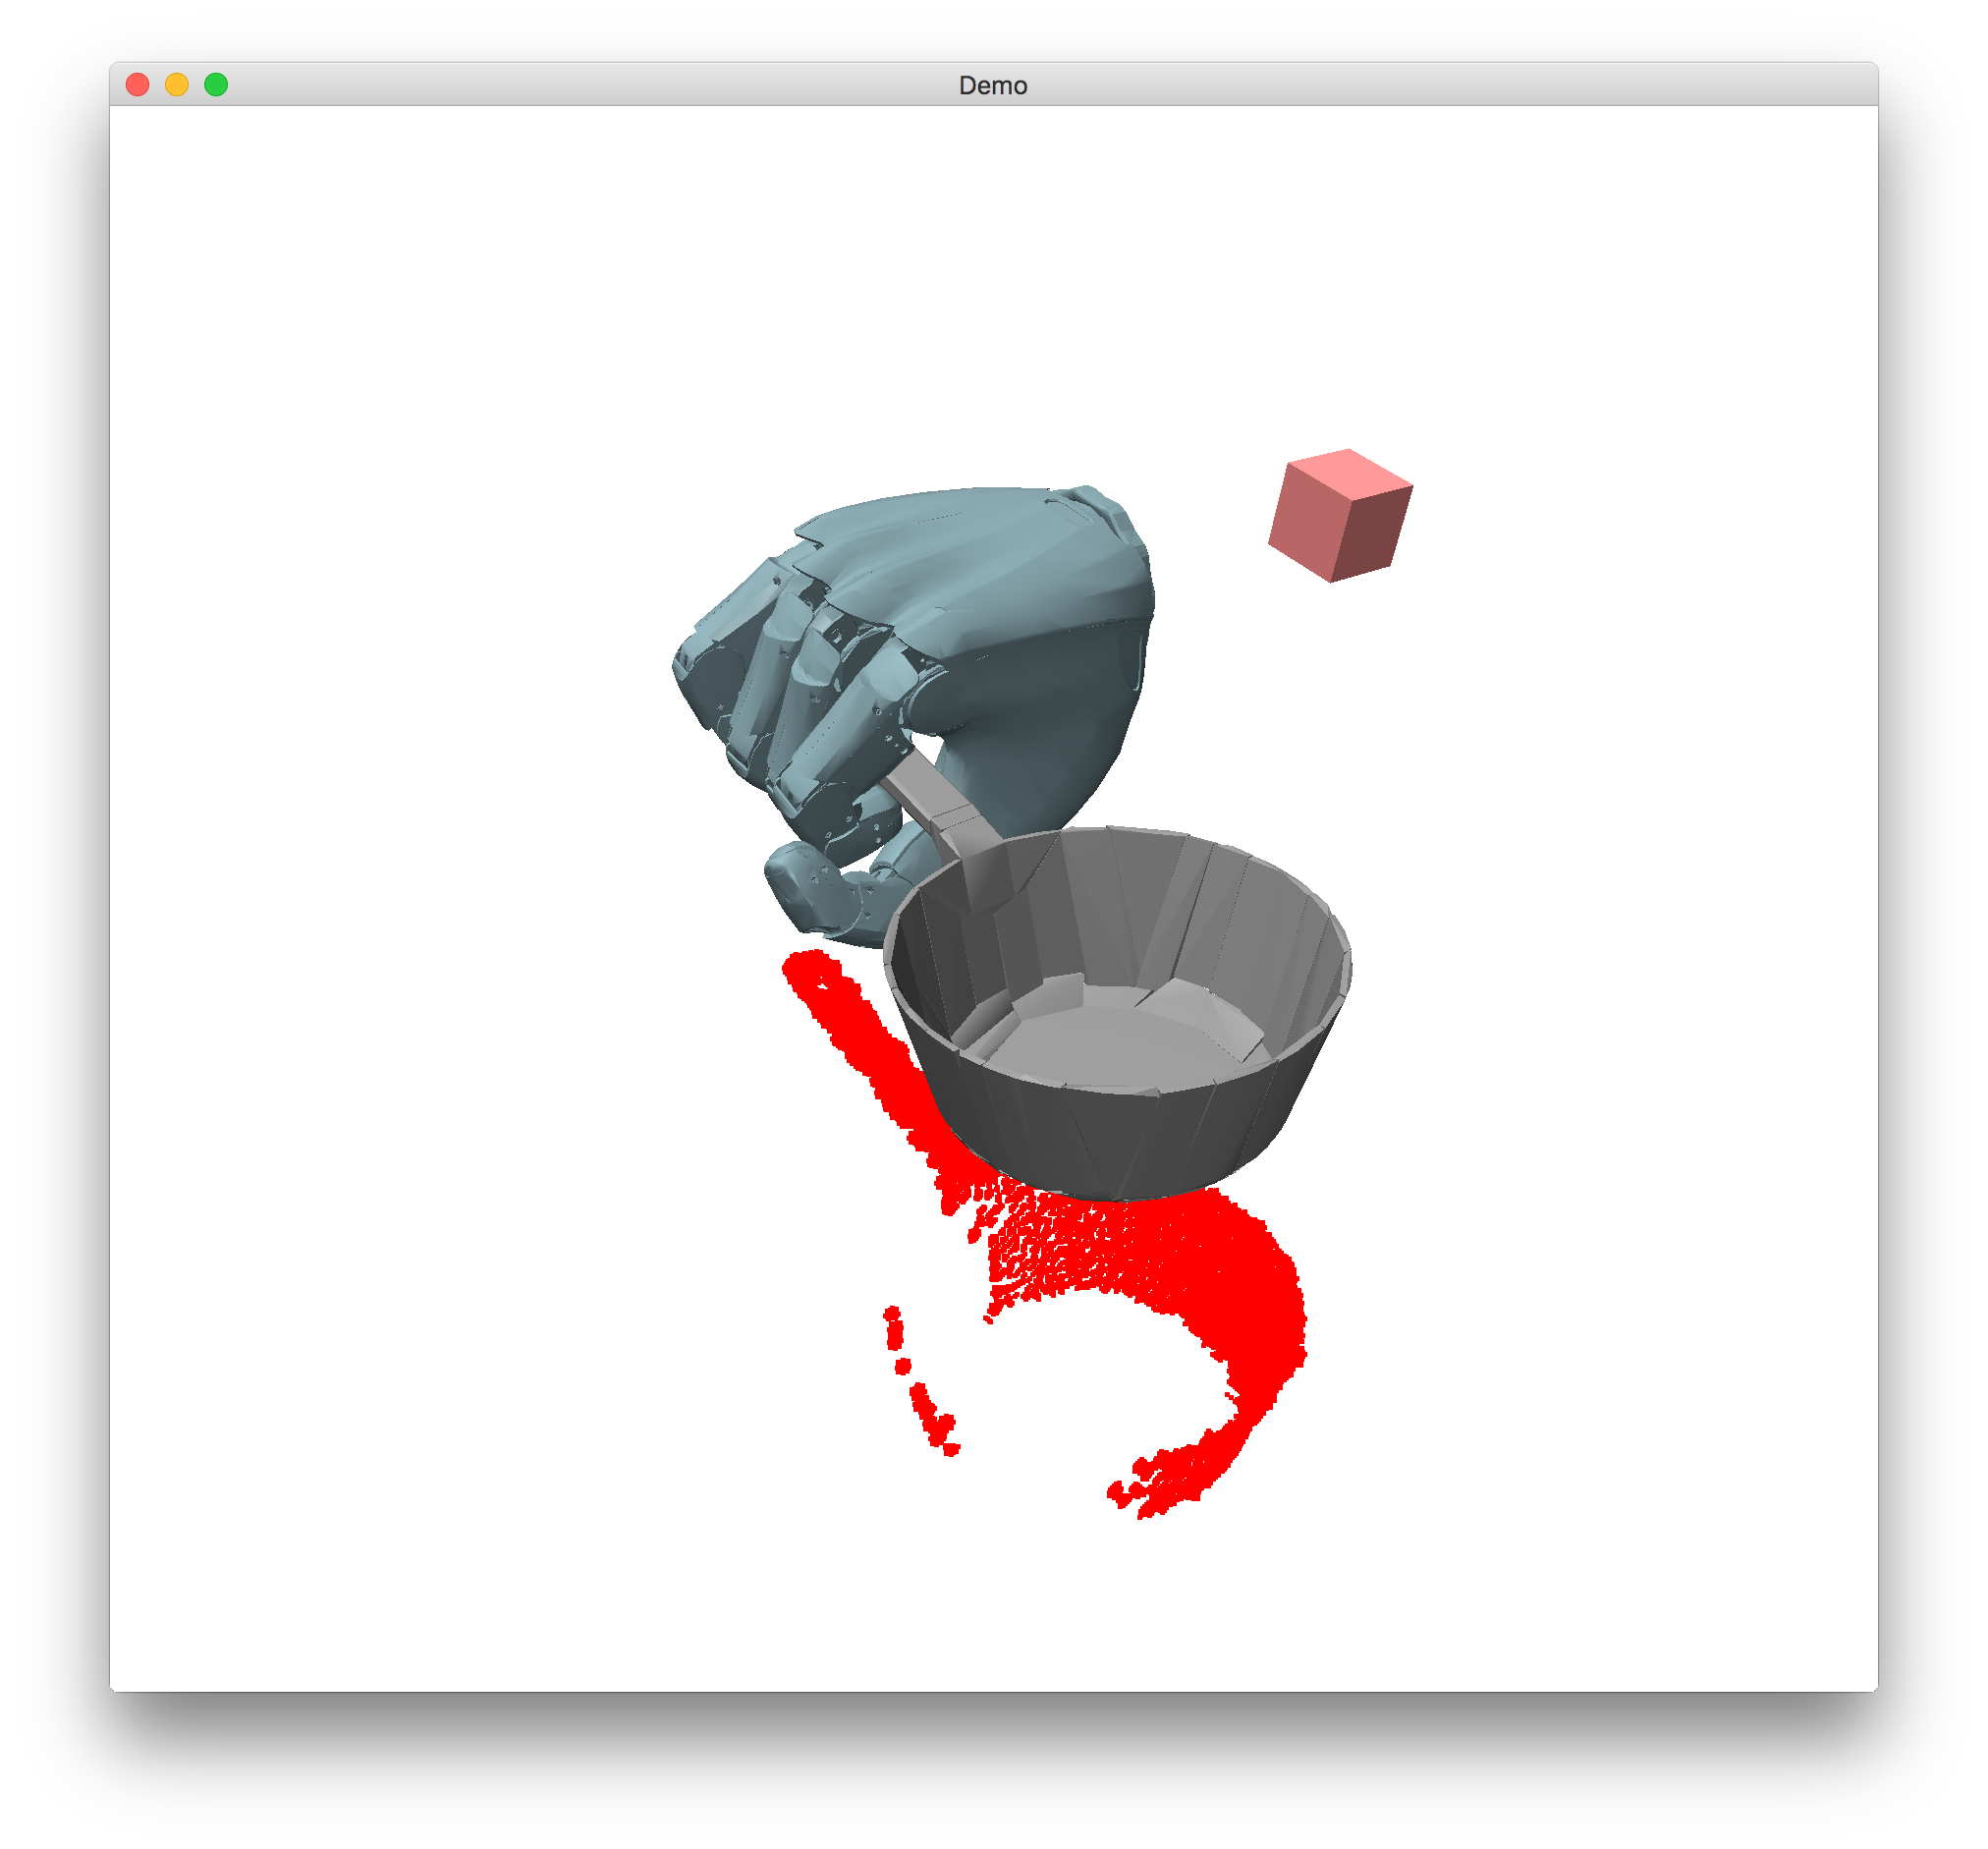
\includegraphics[width=0.24\textwidth]{images/Pan4_HFHW}
%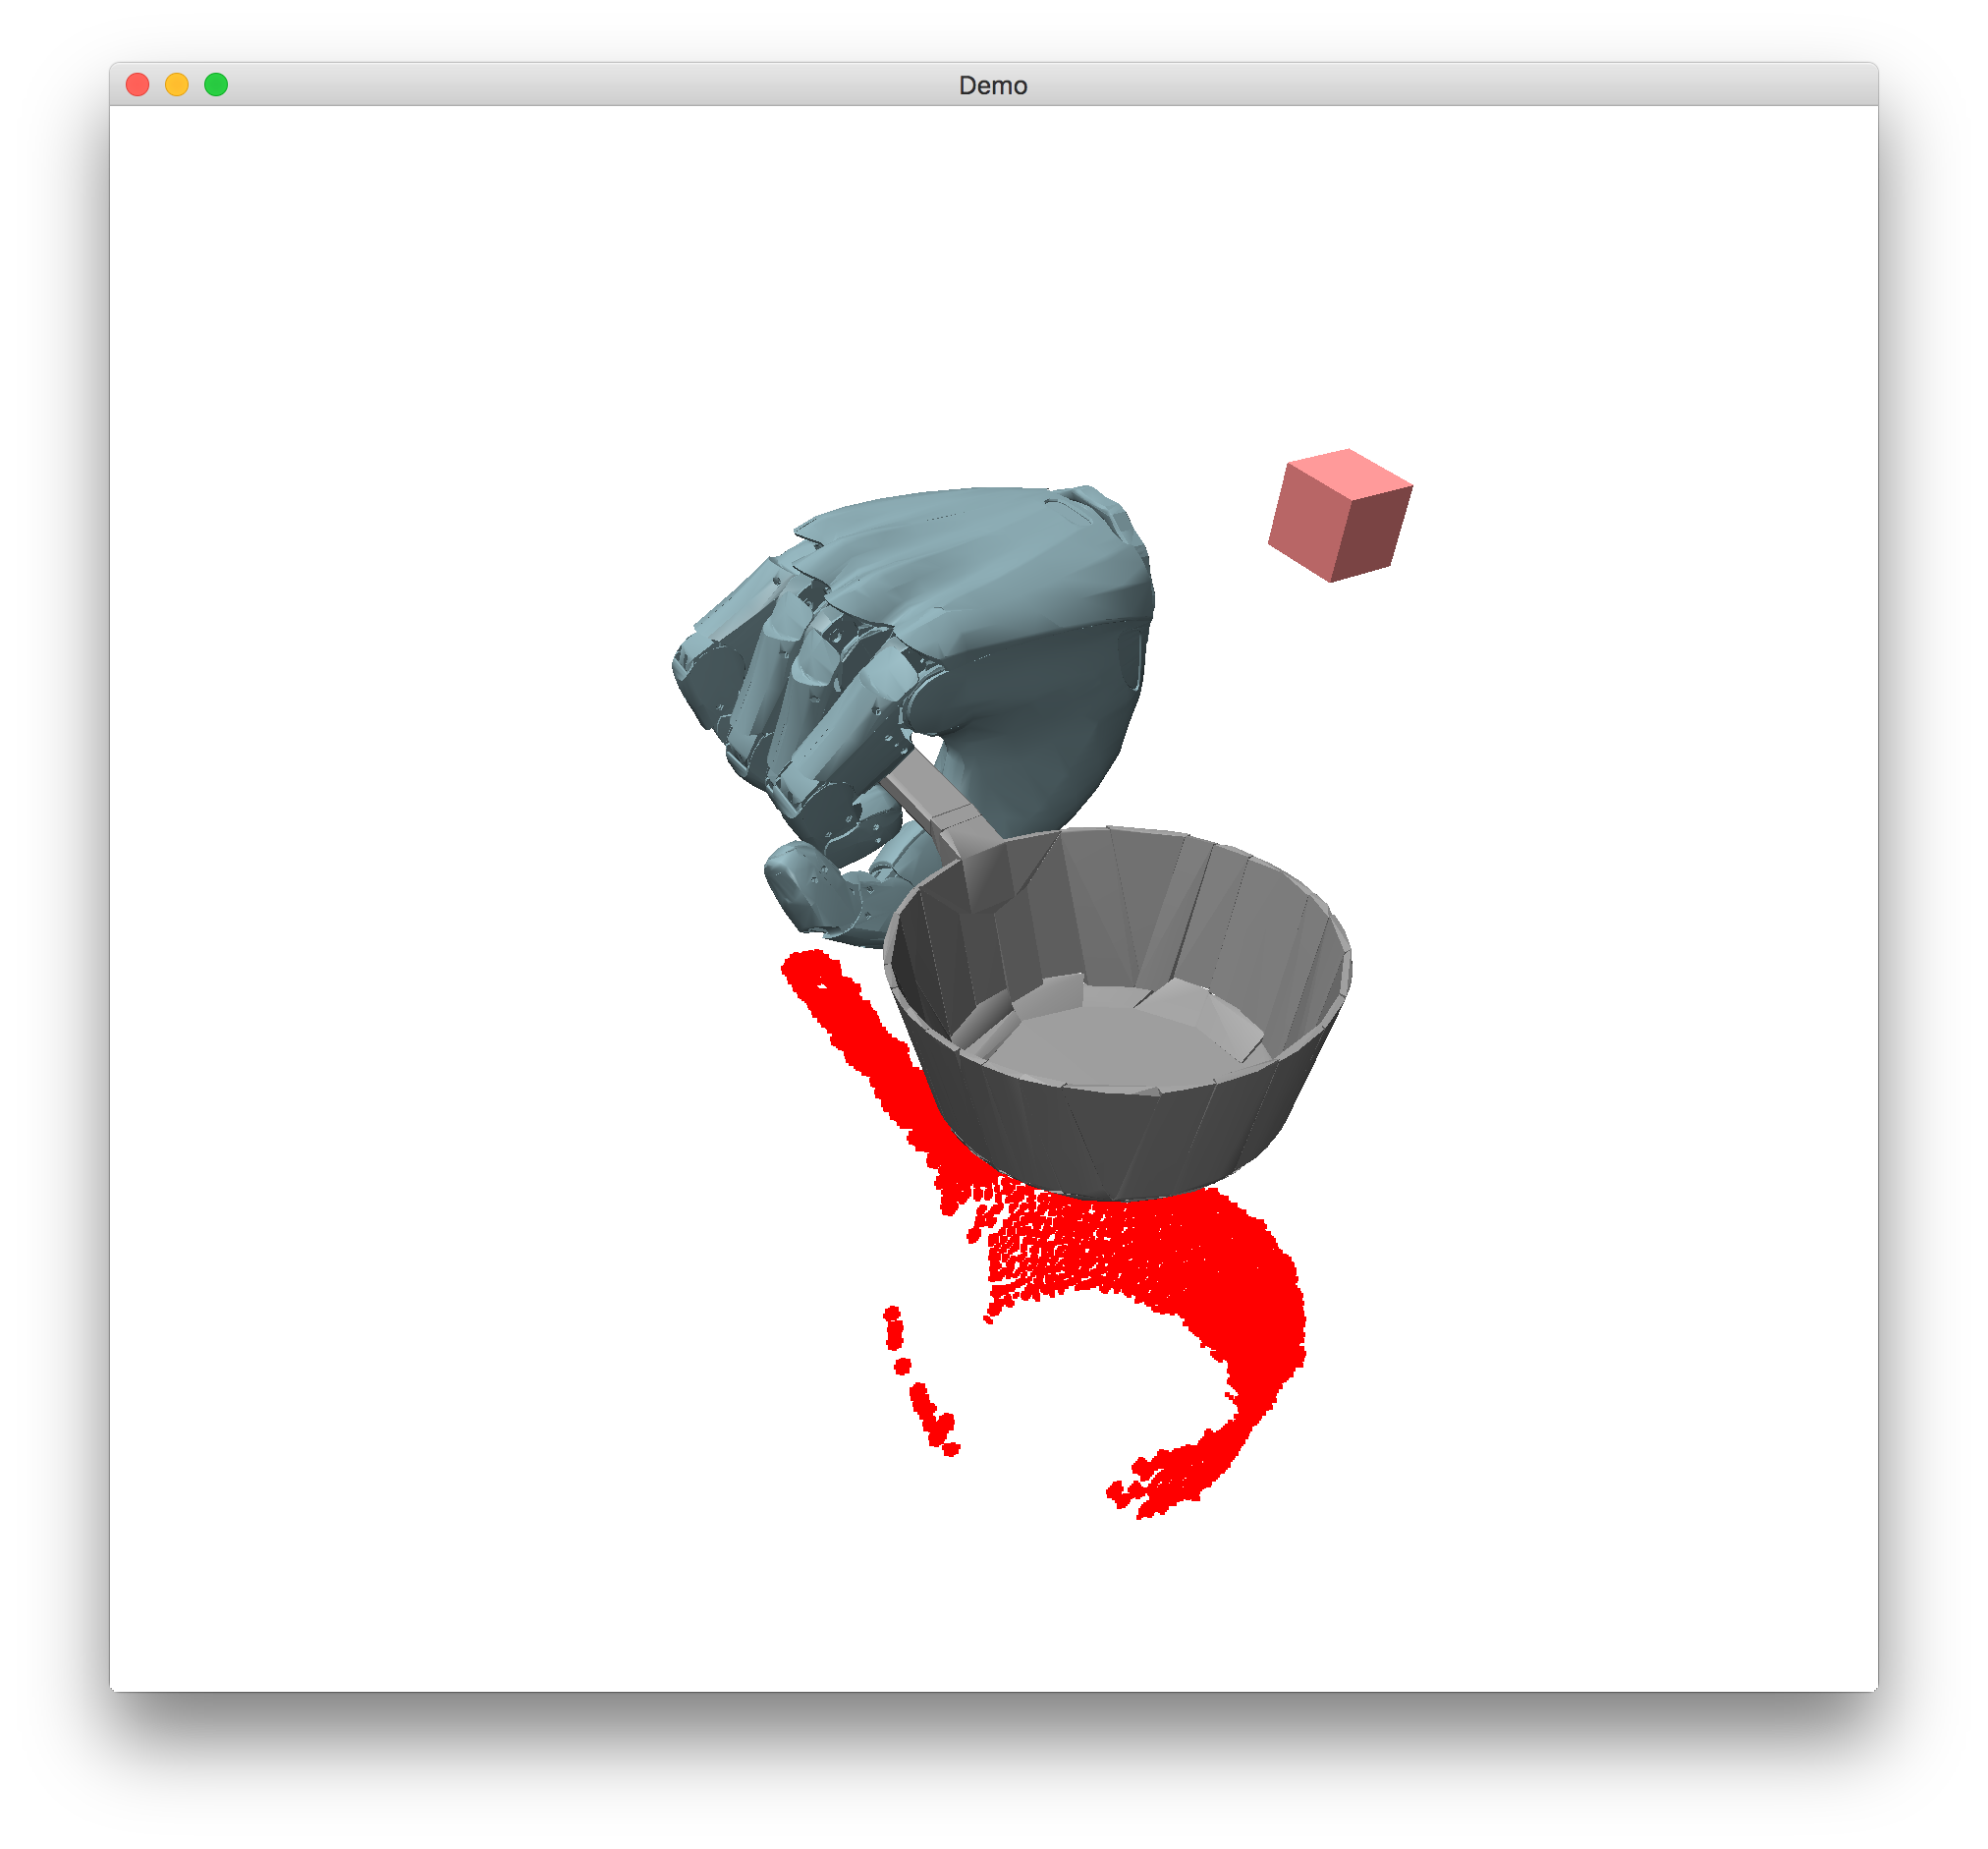
\includegraphics[width=0.24\textwidth]{images/Pan4_LFHW}
\caption{Creating a data set for robust evaluation. (Top row) The same pinch grasp, executed on the same object, with varying friction and mass parameters. (Bottom row) A more robust power grasp, executed on the same object, with the same variation in friction and mass. \label{fig:evaluative-training}}
\end{figure}

Using this method, we generated a data set (DS1) of 1.12 million simulated grasps using GM1 as the generative model and a data set of 1.136 million additional grasps (DS2) using GM2. Each grasp can be replayed in Mujoco and the set can be decomposed for train and test purposes as required. We give details of the statistics in Table including the way that we break down the data-set into training, validation and test subsets. The ratio of successful grasps in the dataset is less than 50\% for GM1, and is more than 50\% for GM2. In order to have a balanced training set, the number of successful and unsuccessful grasps have been equalised by under-sampling the failure cases in GM1 and over-sampling the failure cases for GM1. No balancing was performed for GM1/2 validation and test sets.
\begin{table*}[t]
\centering
\caption{Statistics of the simulated data sets.}
\label{tab:data}
\begin{tabular}{|l|l|l|l|l|l|l|l|l|l|l|} \hline
Data set & Generative &  Subset & \# Scenes & Top-grasp & Top-grasp & Top grasp & Total & Total  & Total  & Total \\ 
              & Model         &              &                   &  \# succs  & \# fails       & \% succs  & grasps   & \# succs      & \# fails  & \% succs  \\ \hline
 DS1-Tr & GM1 & Train & 17714 & 10100 & 7614 & 57.0\% & 959,882 & 479,941 & 479,941 & 50.0\% \\ \hline
 DS1-V  & GM1 & Validate & 1042 & 613 & 429 & 58.8\% & 61,393 & 29,557 & 31,836 & 48.1\% \\ \hline
 DS1-Te & GM1& Test & 1539 & 1070 & 469 & 69.5\% & 99,521 & 48,084 & 51,437 & 48.3\% \\ \hline
 DS2-Tr  & GM2 & Train & 5377 & 3771 & 1606 & 70.1\% & 943,481 & 533,282 & 410,199 & 56.5\% \\ \hline
 DS2-V   & GM2 & Validate & 544 & 378 & 166 & 69.4\% & 68,586 & 39,559 & 29,027 & 57.7\% \\ \hline
 DS2-Te  & GM2 & Test & 988 & 781 & 207 & 79.0\% & 124,137 & 73,836 & 50,301 & 59.5\% \\ \hline
\end{tabular}
\end{table*}

\section{The Generative Evaluative Architecture} \label{section:evaluative}
%In this section we describe how the evaluative models are trained and how we perform gradient descent and stochastic simulated annealing to attempt to improve grasps using the evaluative model.
\noindent
The grasping system proposed, shown in Figure \ref{fig:systemArchitecture}, consists of a learned generative model and an evaluative model. The generative model is a method that generates a number of candidate grasps given a point cloud, as explained in the previous section. An evaluative model is paired with a generative model in order to estimate a probability of success for each candidate grasp. All evaluative models process the visual data and hand trajectory parameters in separate pathways, and combine them to feed into a third processing block to produce the final success probability. In addition, we present techniques for grasp optimisation using the EM as the objective function, using both Gradient Ascent (GA) and Simulated Annealing (SA). Finally, we train each \textcolor{red}{evaluative model with data sets of simulated grasps generated using the generative models GM1 and GM2.} Table \ref{table:GEBreakdown} shows a the full list of 17 variants we test.

In this section, the three proposed evaluative model (EM) architectures are explained. The grasp generator models, GM1 and GM2, given in the previous section, require very little training data to train, here being trained from 10 example grasps. %GM1 can generate 500 candidate grasps, ranked according to their estimated likelihoods, within 10 seconds on a 2x Intel Xeon E5-2650 v2 Eight Core 2.6GHz. GM2 takes a 50 seconds to create 250 grasps in the same setting. 
These generative models do not, however, estimate a probability of success for the generated grasps. An evaluative model, which is a Deep Neural Network (DNN), is used specifically for this purpose. DNNs have shown good performance in learning to evaluate grasps using grippers \cite{levine16,lenz2015deep}. They have also been applied to generating pre-grasps, so as to perform power grasps with dexterous hands \cite{varley2015generating,lu2017planning}.

%The generative approach ignores the global information about the object, such as overall shape and the object category. The success of an executed grasp, however, depends on many contextual factors such as full object shape, mass, mass distribution and surface friction. An evaluative network can indirectly learn to predict grasp success from image data. 
%The data provided to the evaluative network is collected from randomly generated scenes, therefore each scene has a different random combination of the parameters. The primary purpose of the network is to learn robust grasps across different conditions, and this is a complex task. The first challenge is that the kinematic model of the hand is unknown to the evaluative network. It only has access to the parameters that \textit{configure} the hand: the wrist and joint positions. Second, the system is weakly supervised with the grasp result (success or failure), and no further labels are provided.

We tested three evaluative models. The first is based on the VGG-16 network \cite{Simonyan14c}, named Evaluative Model 1 (EM1), and shown in Figure \ref{fig:networkArchitecture2} (a). A version based on the ResNet-50 network, termed EM2, is shown in Figure \ref{fig:networkArchitecture2} (b). Finally, EM3 (Figure \ref{fig:networkArchitecture2} (c)) is also based on VGG-16. All EMs are initialised with ImageNet weights. Regardless of the type, an EM has the functional form $f(I_t, h_t)$, where $I_t$ is a colourised depth image of the object,\footnote{\textcolor{red}{Colourisation is a process by which additional channels are added to create a 3 channel representation. Here we add a channel encoding mean curvature and one encoding Gaussian curvature at that point in the depth image.}} and $h_t$ contains a series of wrist poses and joint configurations for the hand, converted to the camera's frame of reference.The network's output layer calculates a probability of success for the image-grasp pair $I_t$, $h_t$. The model processes the grasp parameters and \textcolor{red}{colourised depth} information in separate channels, and combines them to feed into a feedforward pipeline that produces the output.
\begin{table}[b]
\footnotesize
\centering
\begin{tabular}{|l|l|l|l|l|l|l|}
\hline
Variant & GM/  & EM & Opt'  & Training Set \\ 
 & Testset & & Meth' & \\ \hline
V1 & GM1    & - & - & 10 grasps  \\ \hline
V2 & GM2    & - & - & 10 grasps  \\ \hline
V3 & GM1/DS1-Te & EM1 & - & DS1-Tr \\ \hline
V4 & GM1/DS1-Te & EM2 & - & DS1-Tr \\ \hline
V5 & GM1/DS1-Te & EM3 & - & DS1-Tr  \\ \hline
V6 & GM1/DS1-Te & EM1 & - & DS1-Tr + DS2-Tr \\ \hline
V7 & GM1/DS1-Te & EM2 & - & DS1-Tr + DS2-Tr \\ \hline
V8 & GM1/DS1-Te & EM3 & - & DS1-Tr + DS2-Tr \\ \hline
V9 & GM2/DS2-Te & EM1 & - & DS1-Tr + DS2-Tr \\ \hline
V10 & GM2/DS2-Te & EM2 & - & DS1-Tr + DS2-Tr \\ \hline
V11 & GM2/DS2-Te & EM3 & - & DS1-Tr + DS2-Tr \\ \hline
V12 & GM1/DS1-Te & EM3 & GA1 & DS1-Tr + DS2-Tr \\ \hline
V13 & GM1/DS1-Te & EM3 & GA2 & DS1-Tr + DS2-Tr \\ \hline
V14 & GM1/DS1-Te & EM3 & GA3 & DS1-Tr + DS2-Tr \\ \hline
V15 & GM1/DS1-Te & EM3 & SA1 & DS1-Tr + DS2-Tr \\ \hline
V16 & GM1/DS1-Te & EM3 & SA2 & DS1-Tr + DS2-Tr \\ \hline
V17 & GM1/DS1-Te & EM3 & SA3 & DS1-Tr + DS2-Tr \\ \hline
\end{tabular}
\caption{The evaluated combinations of architecture, generative model/test set, training set, and optimisation method (Gradient Ascent (GA) or Stochastic Simulated Annealing (SA).}
\label{table:GEBreakdown}
\end{table}

%\begin{figure}[h]
%  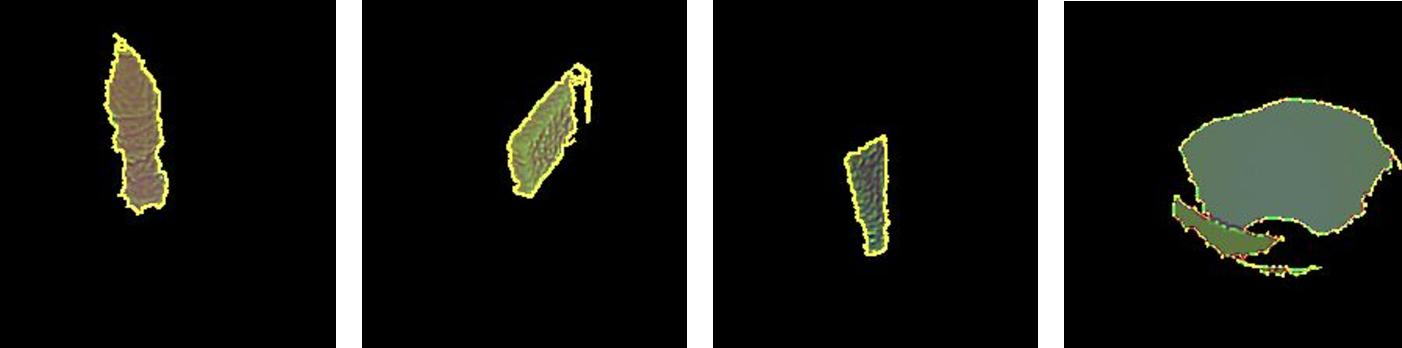
\includegraphics[width=0.9\linewidth]{images/colourDepth.pdf}
%  \caption[Colourised depth images.]{Colourised depth images. From left to right, the objects are: coke bottle, chocolate box, hand cream, and bowl.}
%\label{fig:colorisedDepth}
%\end{figure}
The single-channel depth image is colourised before it is passed as input to the evaluative network. For this, we first crop the middle $460 \times 460$ section of the $640 \times 480$ depth image, and down-sample it to $224 \times 224$. Two more channels of the same dimensions are added, corresponding to \textcolor{red}{the mean curvature and the Gaussian curvature}. %Figure~\ref{fig:colorisedDepth} contains four examples of colourised depth images. 
This procedure provides meaningful depth features to the network, and makes the input compatible with VGG-16 and ResNet-50, which require input images of size $224 \times 224 \times 3$.

The grasp parameter data $h_t$ consists of 10 trajectory waypoints represented by $27 \times 10 = 270$ floating point numbers, and 10 extra numbers reserved for the grasp type.\footnote{\textcolor{red}{Hand trajectory parameters are represented in the camera frame. Each waypoint has 27 float values: wrist position $(x,y,z)$ , wrist orientation (quaternion); finger joint angles (4 joints per finger, 5 fingers). Overall: 280 (10 + 10 * 27) floats per grasp.}} \textcolor{red}{Using trajectory information gives the network information it can use to predict unanticipated collisions with the object that will cause the grasp to fail.} Each of the 10 training grasps is treated as a different class, and $h_t$ uses the 1-of-N encoding system. The grasp parameters are converted to the coordinate system of the camera which was used to obtain the corresponding depth image. In EM1 and EM2, the parameters are processed with a fully-connected (FC-1024) layer and \textit{element-wise added} to the \textcolor{red}{learned} visual \textcolor{red}{representations}, while EM3 uses a convolutional approach. All networks join the \textcolor{red}{learned} visual features and grasp parameters in higher layers.

All FC layers have RELU activation functions, except for the output, which uses 2-way softmax in all EM variants. The output layer has two nodes, corresponding to the grasp success and failure probabilities. Cross-entropy loss is used. % to train the neural network, as given in \eq\ref{equation:crossentropy}.

All evaluative models in Table \ref{table:GEBreakdown} were trained and tested on simulated data. EM2 and EM3 were tested on the real robot setup. Variants V3-V5 were trained using DS1-Tr. Variants V6-V17 were trained using the combined data set from DS1-Tr and DS2-Tr \footnote{10\% of DS1-Tr failure cases were sampled from the grasps that collide with the table, and we preserved the colliding grasps in DS1-V. This was to ensure EMs do not propose such grasps. Training with DS2 did not involve colliding grasps since overall grasp quality of GM2 is better.}. The Gradient Descent(GD) optimiser was employed with starting learning rate of 0.01, a dropout rate of 0.5, and early stopping. We halve the learning rate every 5 epochs during training.


%\begin{equation}
%H_{y'}(y) := - \sum_{i} ({y_i' \log(y_i) + (1-y_i') \log (1-y_i)})
%\label{equation:crossentropy}
%\end{equation}
%where $y_i'$ is the class label of the grasp, which is either 1 (success) or 0 (failure), and $y_i = f(I_i, h_i)$ is is the predicted label of the grasp pair ($I_i$, $h_i)$.
The models are introduced below. Only their unique properties are highlighted.

\begin{figure*}[t!]
\centering
% \begin{center}
\subfloat[Evaluative Model 1]{%
  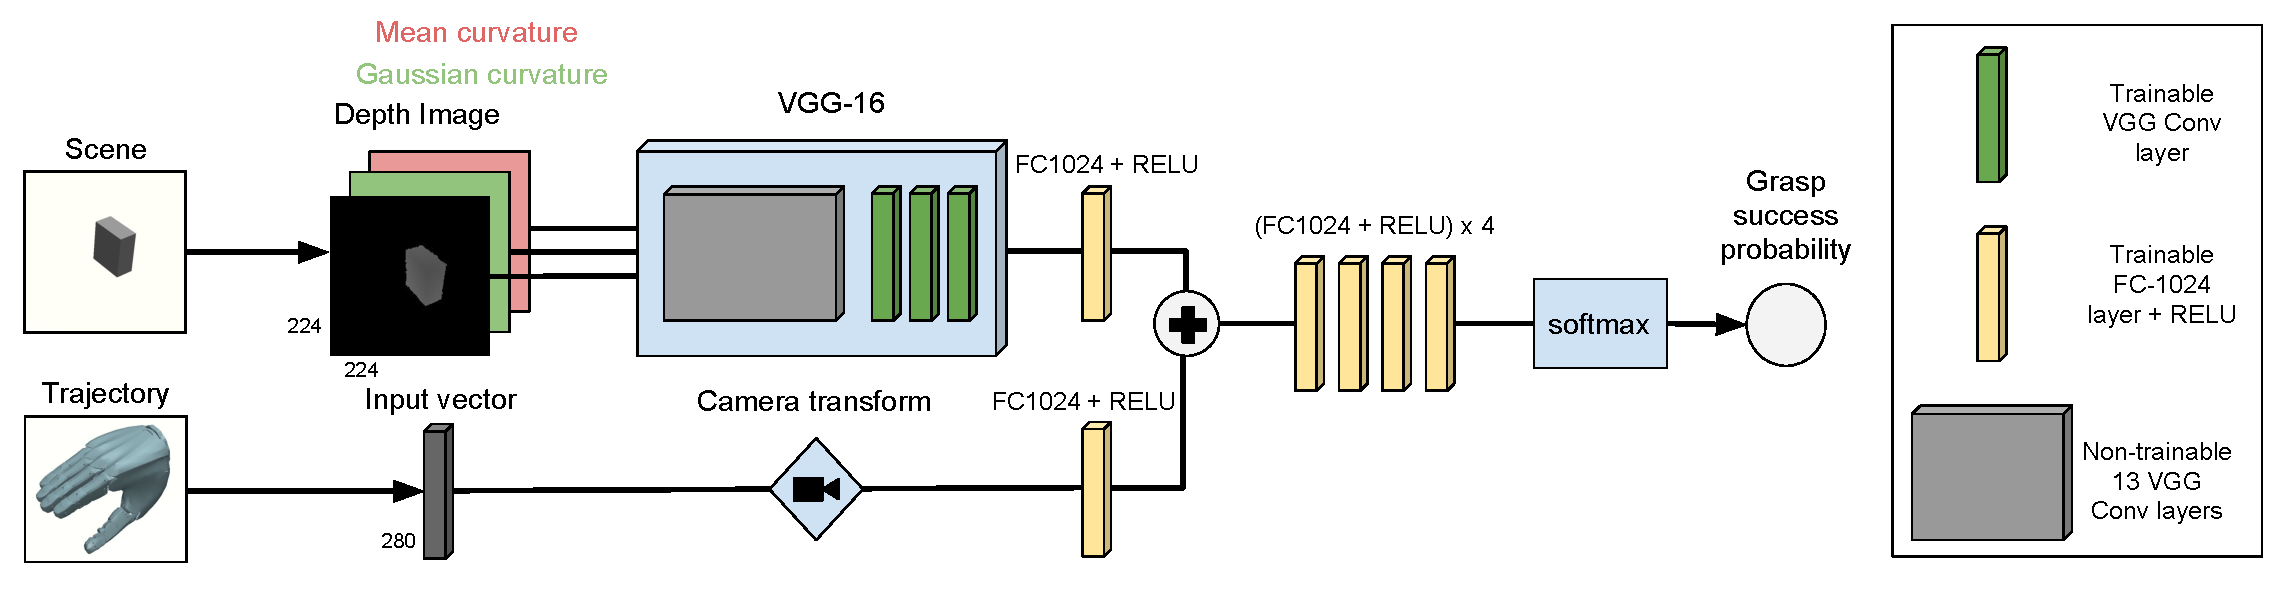
\includegraphics[width=0.91\textwidth]{images/networkArchitecture.pdf}
}
% \end{center}

% \begin{center}
\subfloat[Evaluative Model 2]{%
    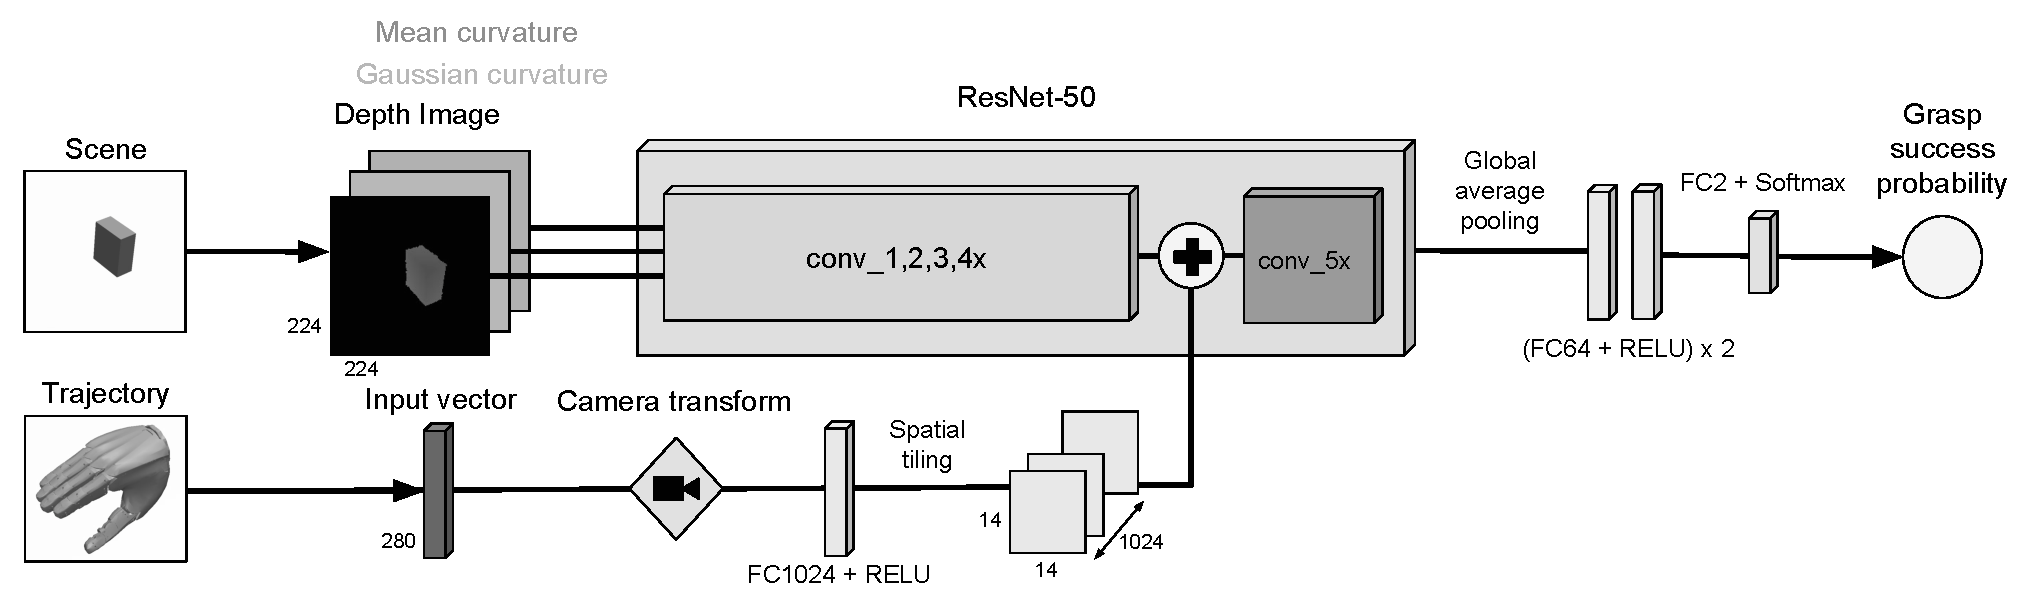
\includegraphics[width=0.91\textwidth]{images/ResNet.pdf}
}
% \end{center}

% \begin{center}
\subfloat[Evaluative Model 3]{%
    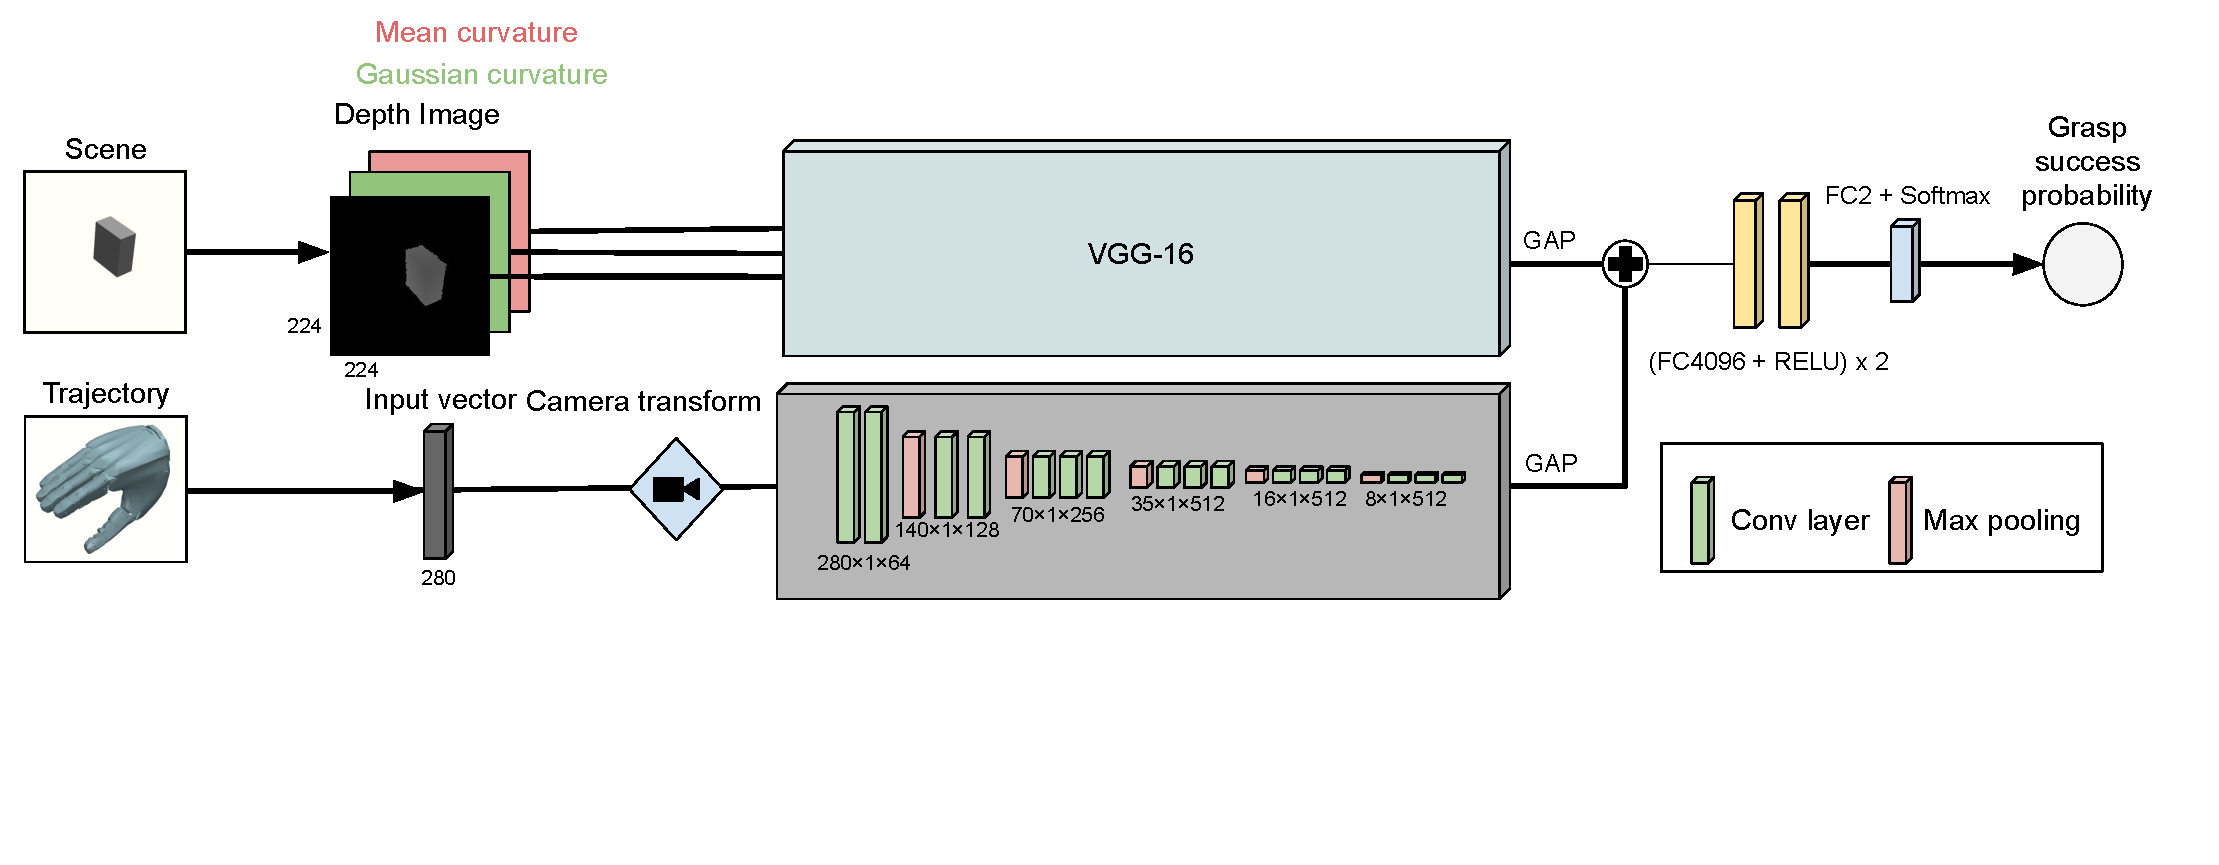
\includegraphics[width=0.91\textwidth]{images/Chaonet_newpic.pdf}
}
% \end{center}
\caption{The three evaluative network architectures. (a) EM1, a VGG-16 based model, where the first 13 layers of VGG-16 are frozen. (b) EM2, a ResNet-50-based network. The first four blocks are used for feature extraction and the rest to learn joint features. (c) EM3, also based on VGG-16.}
\label{fig:networkArchitecture2}
\end{figure*}

\subsection{Evaluative Models}

\noindent {\bf Evaluative Model 1 (EM1).}
\noindent
Figure~\ref{fig:networkArchitecture2} (a) shows the architecture of the first evaluative network. The colourised depth image is processed with the VGG-16 network \cite{Simonyan14c}. The first 13 layers are frozen to reduce overfitting. Grasp parameters and image features each pass through two FC-1024 layers to obtain two feature vectors of length 1024. The features are combined using element-wise addition and fed into 4 FC-1024 layers. Concatenation and addition can be considered as interchangeable in this context \cite{dumoulin2018feature-wise}. The final FC-1024 layers form associations between visual features and hand parameters, and contain most of the trainable parameters in the network.

\noindent {\bf Evaluative Model 2 (EM2).}
\noindent
% \begin{figure}[!ht]
%   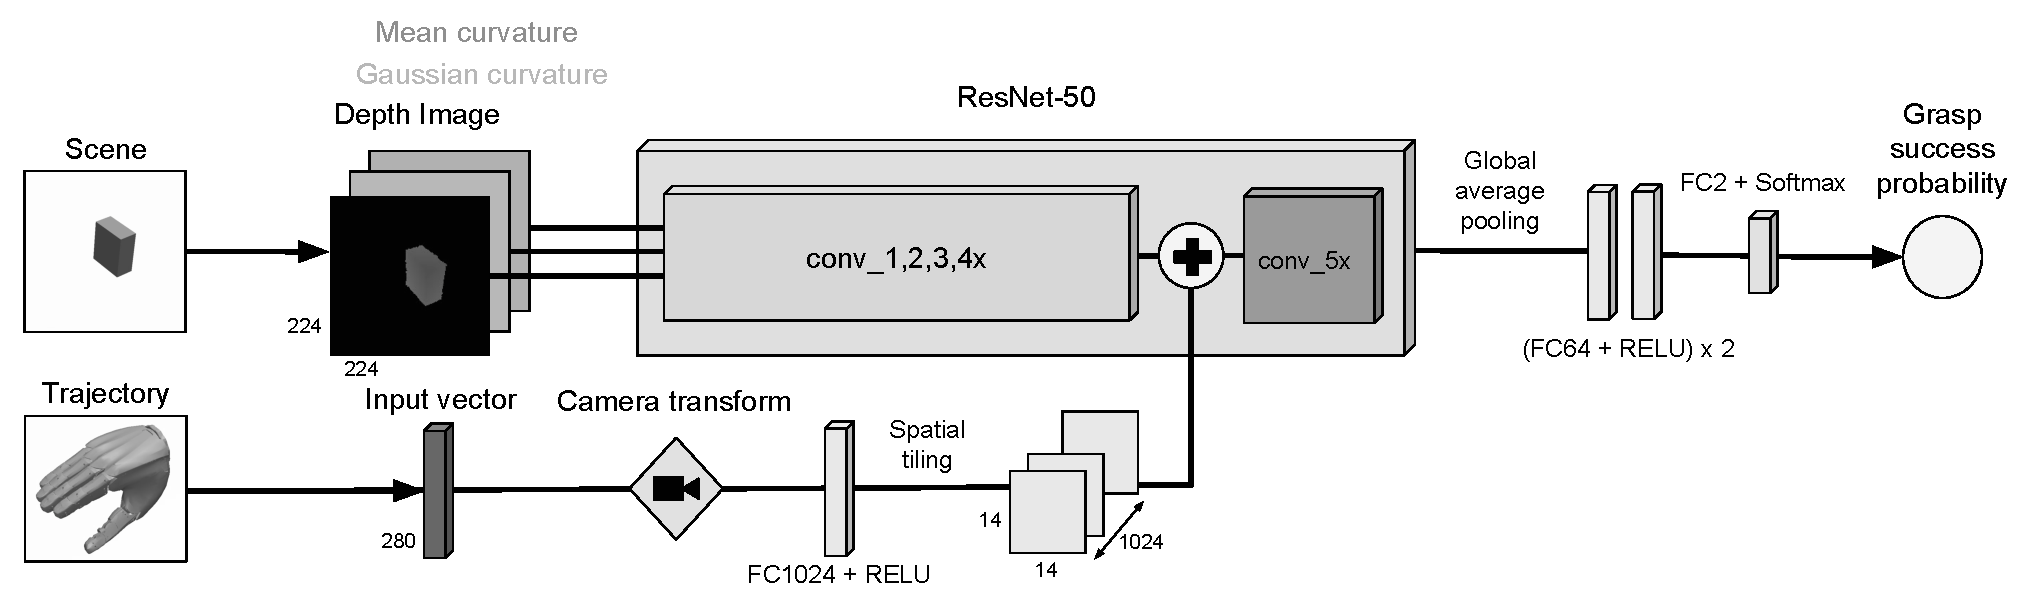
\includegraphics[width=\textwidth]{images/ResNet.pdf}
%   \caption[The ResNet-based evaluative deep neural network architecture.]{The ResNet-based evaluative deep neural network architecture (EM2). Spatial tiling is used to repeat the grasp parameters before they join the image processing pathway. This network requires fewer FC layers due to the earlier marriage of information channels.}
% \label{fig:ResNet}
% \end{figure}
EM2 (Figure~\ref{fig:networkArchitecture2} (b)) uses the ResNet-50 architecture \cite{HeZRS15}, broken down into two parts. The first 4 convolutional blocks are used to extract the visual features. The final block, with 9 randomly-initialised convolutional layers, combines these with the grasp parameters. Similar to EM1, element-wise addition joins the two channels. The grasp parameters, a vector of size $1024$, are repeated to form a block of size $14 \times 14 \times 1024$. The final block processes the merged information and has 2 FC-64 layers.

\noindent {\bf Evaluative Model 3 (EM3).}
\noindent
This model (Figure~\ref{fig:networkArchitecture2} (c)) also uses VGG-16, but all 16 layers are trainable. The hand trajectory parameters pass through a feature extraction network before being concatenated with the visual features. The combined part of the network contains two high-capacity FC-4096 layers, followed by a FC2+softmax layer. EM3, in contrast to EM1 and EM2, uses convolutional layers for processing input grasp trajectories. The trajectory sub-network is similar to VGG-16 in that it contains 5 blocks, comprising 13 convolutional layers. The convolutional filters have a width of 3. The sizes under the blocks are input dimensions. Global Average Pooling (GAP) is used to obtain 512 features from each side, which are concatenated and passed through two FC-4096 layers. 

\subsection{Grasp optimisation using the EM}
\noindent
So far we have considered only generative-evaluative architectures where the evaluative model (EM) merely ranks the grasp proposals. As proposed by Lu et al. \cite{lu2017planning} \textcolor{red}{the EM can be used to improve grasp proposals}. This boils down to searching the grasp space driven by the EM as the objective function. This may be by gradient ascent or simulated annealing. The methods V12-17 use V8 as the objective function, hence V8 should be treated as the baseline. We employed both gradient based optimisation and simulated annealing.

\subsubsection{Gradient based optimisation}
\noindent
Lu et al. \cite{lu2017planning} proposed gradient ascent (GA), modifying the grasp parameters input to the EM with respect to the output, predicted success probability. They initialised with a heuristically selected pre-grasp. \textcolor{red}{It is an interesting question whether we can apply their method to our evaluative models so as to further improve the performance. We therefore apply their technique initialised with the highest ranked grasp according to the EM.} We investigated three variants:
\begin{itemize}
\item GA1: Shifts the position of all of the waypoints in the grasp trajectory equally. The gradient is the average position gradient across all 10 waypoints.
\item GA2: Tunes the hand configuration by tuning the angle of each finger joint. Every finger joint at each waypoint is treated independently.
\item GA3: Performs GA1 and GA2 simultaneously.
\end{itemize}

\subsubsection{Simulated annealing based optimisation}
\noindent
Gradient based optimisation is sensitive to the quality of gradient estimates derived from the model. Simulated annealing (SA) based optimisation is more robust to such noise. Therefore, three optimisation routines were implemented using SA:
\begin{itemize}
\item SA1: Shifts the positions of the all waypoints in the grasp trajectory equally. Moves are drawn from a three-dimensional Gaussian with $\mu=0$ and $\sigma=0.001$. 
\item SA2: Scales the angles of the finger joints in the final grasp pose with a single scaling parameter drawn from a Gaussian with $\mu=1$ and $\sigma=0.001$. The initial finger joint angles remain fixed and joint angles of the intermediate waypoints are linearly interpolated. 
\item SA3: Performs SA1 and SA2 simultaneously.
\end{itemize}


\section{Simulation Analysis}
\label{section:simulationAnalysis}
This section presents a simulation analysis of the various architectures based on the two data sets. 
We assess each variant in two different ways. First, for any method with an evaluative model we  measure the prediction accuracy of the EM. We compare the actual outcomes in a test set with the EM's prediction as to whether it is more likely to succeed or fail (output set at a threshold of 0.5). This gives us a confusion matrix from which we can calculated sensitivity, specificity and F1 score. Second, since a robot can only execute one grasp, we can measure the proportion of successful top-ranked grasps for any method. In each analysis the test set effectively replaces the Generative Model as it contains, for any scene, a complete list of grasps. Thus TS1 contains grasps proposed by GM1 and TS2 contains grasps proposed by GM2. This allows us to simulate the effect of different generative models on performance. 

We performed both analyses and the results are given in Table~\ref{table:Results-sim}. When assessing pure GM architectures, we can only measure the top ranked grasp success, since the GMs give a grasp likelihood according to the generative model not a probability of success. 

The main findings are as follows. First, of the pure generative models GM2 outperforms GM1, with top ranked grasp successes of 79.05\% and 69.53\% respectively. Second, the GEA architectures all outperform both pure GM architectures, starting at 87.85\% of grasps succeeding (V3 based on proposals from GM1 and evaluation by EM3 trained on TS1). Third, the increase in training set size (adding GM2 to GM1) yields a further improvement. We can best measure this by considering the residual number of top grasps that fail as a percentage of the baseline (GM1). On this measure adding the additional data (variants V6-V9) improves performance (over variants V3-V5) by an average of 3\%. 

All the above results use GM1 as the generative model. We can measure the benefit of substituting this by GM2. This yields a further reduction in residual failures over GM1 under the same training conditions (training with DS1-Tr and DS2-Tr) of 3.5\%. 

In summary, simulation results provide evidence that: pure GM2 outperforms GM1; adding training data improves results; and using GM2 as the generative model in the generative-evaluative architecture improves results. 

%Recall that the generative-evaluative architecture (GEA) comprises both the generative model (GM) and the evaluative model (EM). 
%We can evaluate aspects of these separately. After training, the EM was used to predict grasp outcomes in the test set. This comprised 1,241 scenes with 76,213 grasps. Of these, 40,243 succeeded and 35,970 failed. Our analysis is given in Table~\ref{fig:predictions}. The sensitivity is 0.84 and the specificity 0.71. The F1-score is 0.802.
%\begin{table}[b]
%\centering
%\caption{Confusion matrix for prediction on simulated data.}
%\label{fig:predictions}
%\begin{tabular}{|c|c|c|c|c|c|}
%\hline
% & & \multicolumn{4}{c|}{Prediction} \\ \cline{3-6}
%      & & \multicolumn{2}{c|}{\#} & \multicolumn{2}{c|}{\%} \\ \cline{3-6}
%  &  & Succ         & Fail         & Succ         & Fail         \\ \hline
%\multirow{ 2}{*}{Ground Truth} \newline & Succ & 33890      & 6353       & 84\%     & 16\%       \\ \cline{2-6}
% &Fail & 10339      &  25631    & 29\%     &  71\%   \\ \hline
%\end{tabular}
%\end{table}
% In this context, precision is the fraction of correctly labeled grasps among those predicted to be of a certain class (success or failure). Recall stands for the fraction of relevant grasps that have been identified correctly among all grasps that belong to that class. The results show a high recall rate for successful grasps, and there are relatively more false positives than false negatives. This necessitates pairing our evaluative neural network with a generative model rather than a random grasp generator, which would likely result in very low quality grasps and consequently, more false positives. 

%To test our generative-evaluative learning architecture we compared the grasp it proposes to the grasp proposed by the generative learner alone. Since \citet{kopicki2015ijrr} showed a 77.7\% success rate with the original generative algorithm we generated a new test set that contained both more challenging objects and placed them in challenging poses. The difficulty single-view grasping with a depth camera depends greatly on the pose of the object relative to the camera. The set comprised 40 test objects (Figure~\ref{fig:real-objects}) and another six training objects. The training objects were used by the human to demonstrate ten example grasps (Figure~\ref{fig:generative-training}). The 40 test objects were used to generate 49 object-pose pairs. From the 40 objects, 35 belonged to object classes in the simulation dataset, while the remaining five do not. 

\begin{figure}[t]
  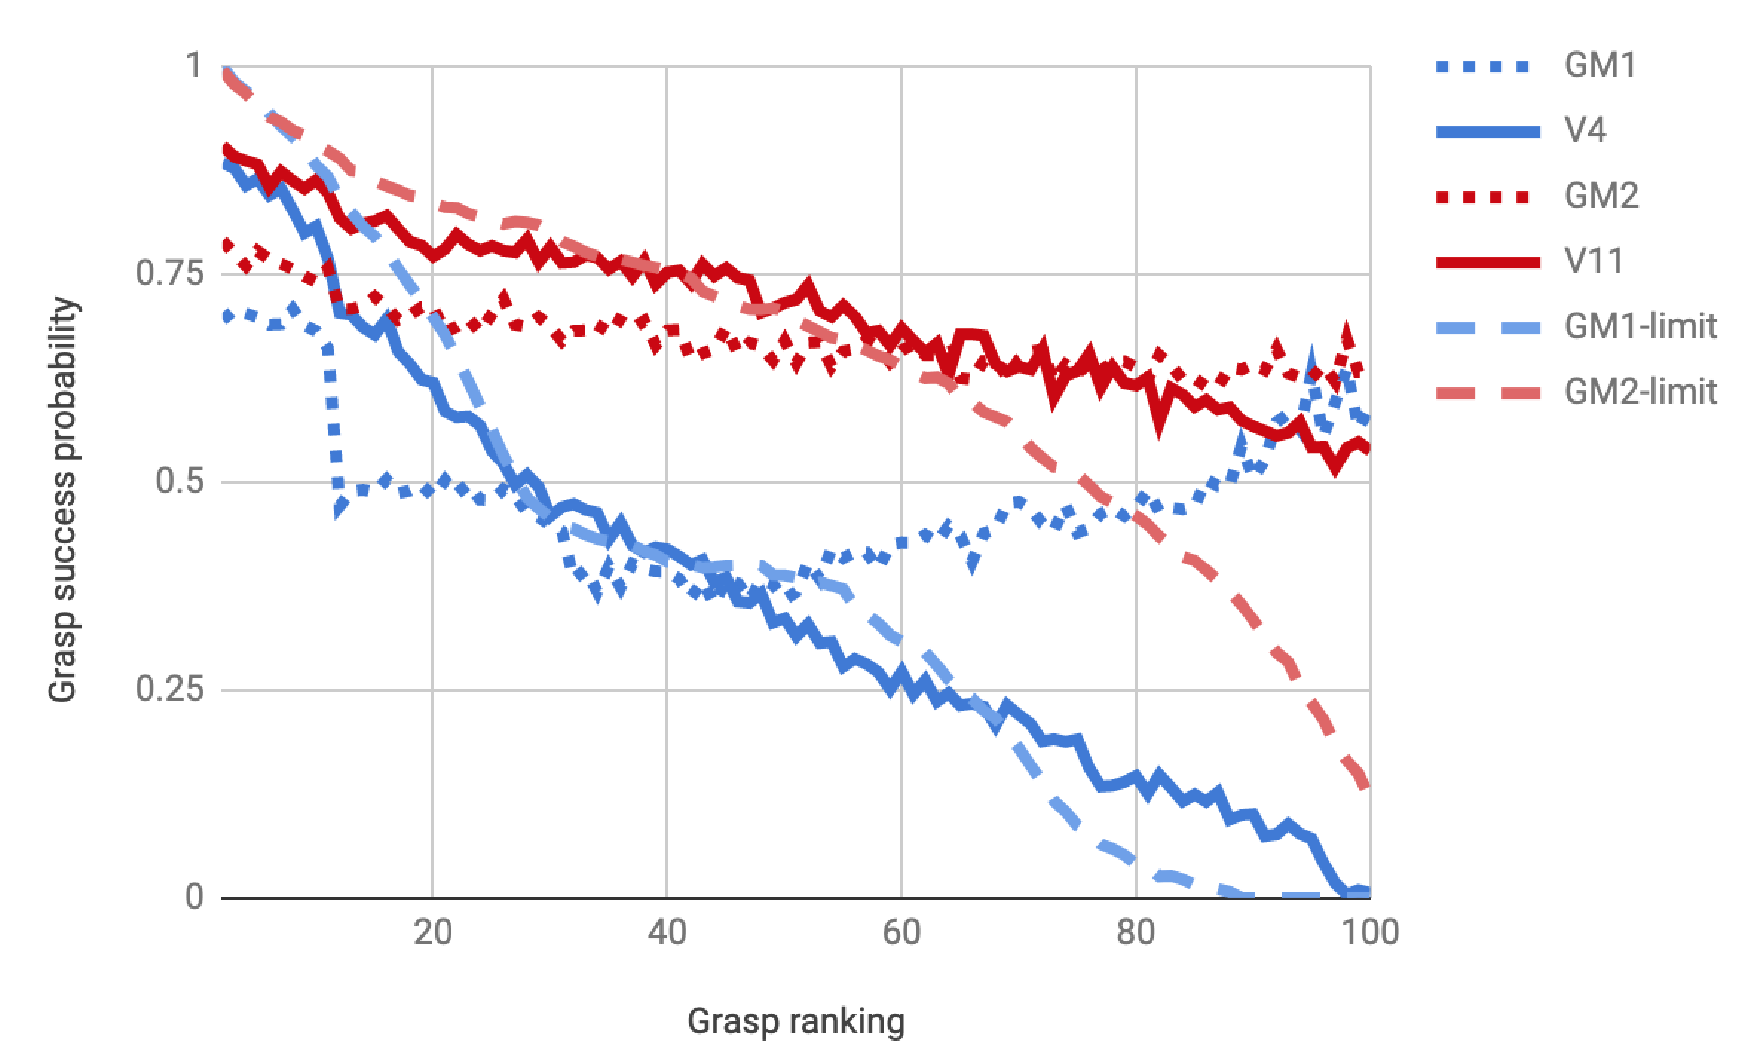
\includegraphics[width=\linewidth]{images/successvsranking.pdf}
  \caption{Grasp success probability (in simulation) vs. grasp ranking. GEA2 and GEA3 use GM1 and GM2 test data, respectively.}
  \label{fig:successvsranking}
\end{figure}

%We compared the EM and GM rankings (Figure~\ref{fig:successvsranking}). The x-axis shows the ranking. The y-axis shows the average actual success rate over all scenes (1,241 test, 7,311 training). When ranked by the EM, the grasp success probability falls nearly monotonically, as is desirable. On the other hand, the likelihood-based ranking of GM results in many good grasps being low-ranked. We also wish to know whether the grasps recommended by the EM and the GM have different grasp success rates. The success rates of the top-ranked grasps are 71.59\% (GM) and  84.2\% (EM).
So far we have considered only Generative-Evaluative architectures where the Evaluative Model merely ranks the grasp proposals. We also investigated using the EM to improve these grasps proposals. This essentially boils down to searching the grasp space driven by the EM as the objective function. This can be done either by gradient descent or using simulated annealing. The methods V12-17 use V11 as the objective function, hence V11 should be treated as the baseline. 

Lu et al. \cite{lu2017planning} proposed gradient ascent on the input grasp parameters to the EM with respect to the predicted success probability. They initialised with a heuristic grasp. We initialise with the best grasp proposed by the GEA. We experimented with three variants of the gradient ascent based tuning:
\begin{itemize}
\item GD1: Moves the entire trajectory at once in the world coordinate space, as directed by the average gradient on the trajectory's all 10 waypoints.
\item GD2: Tunes each finger joint individually. Each waypoint is treated independently.
\item GD3: Performs GD1 and GD2 simulatenously.
\end{itemize}

We ran the optimisation for 50 iterations, using a learning rate of 0.001 for position inputs and 0.01 for finger joints (We used different learning rates since the parameters are in different scales, GD1 in meters and GD2 in radians). Although predicted success rate rises, the success rate in simulation declines in all trials. We observed that the position changes have a more significant negative impact on the grasp success rate, when compared to finger joint movements. The results suggest that optimising dexterous grasps by the EM is non-trivial, perhaps because of the high-dimensionality of the grasp space. We speculate that initialising with a random grasp would be even worse.

Additionally, we implemented three variants of simulated annealing based optimisation:
\begin{itemize}
\item SA1: Moves the entire trajectory at once in the world coordinate space, using a three-dimensional Gaussian noise vector, with $\mu=0$ and $\sigma=0.001$. 
\item SA2: Perturbs the finger joints along the entire trajectory. The pose of all joints in a finger with respect to a reference pose (fully open hand) is modified, which results in an "opening/closing the finger" effect. We observed that this is a more natural movement rather than modifying a finger's joints independently. The opening/closing ratio for each finger is determined by a noise vector that is drawn from a Gaussian distribution with $\mu=0$ and $\sigma=0.01$. 
\item SA3: Performs SA1 and SA2 simulatenously.
\end{itemize}

The simulated annealing procedure contains up to 5 iterations, with 20 random perturbations in each. We start with a temperature of 0.2 and decrease it exponentially to 0.005 by halving it after every batch. If the current solution does not improve after three iterations, the optimisation stops. We do not accept any perturbations that will result in a collision with the table. Similarly with gradient ascent, the performance of the optimised grasps are worse than the baseline (V11). The effect of moving the trajectory is more significant when compared to the finger joints. TODO: Interpret the results.

\begin{table*}[t]
\centering
\begin{tabular}{|l|l|l|l|l|l|l|l|l|l|l|}
\hline
Variant \# & \multicolumn{2}{|c|}{Selected grasp} &  Succ \% & Residual Fails & Test set / GM& \multicolumn{5}{|c|}{Prediction Performance} \\ \hline
 & Succs & Fails &  & as \% of V1 fails &  & TP & FP & TN & FN & Accuracy \\ \hline
V1 & 1070   & 469 & 69.53\% & 100\% & GM1 & - & - & - & - & - \\ \hline
V2 &  781   & 207 & 79.05\% & 68.7\% & GM2 & - & - & - & - & - \\ \hline
V3 & 1352 & 187 & 87.85\% & 39.9\% & GM1 & 37840 &	12226 & 39211 & 10244 & 77.42\% \\ \hline
V4 &  1361 & 178 & 88.43\% & 38.0\% & GM1 & 40234 &	14475 & 36962 & 7850 & 77.57\% \\ \hline

V5 & 1361 & 178 & 88.43\% & 38.0\%& GM1 & 39603 & 14122 &37315 & 8481	& 77.29\% \\ \hline

V6 & 1375 & 164 & 89.34\% & 35.0\% & GM1 & 37584 &	11514 & 39923 &10500	& 77.88\% \\ \hline
V7 & 1363 & 176 & 88.56\% & 37.5\% & GM1 & 39332 &	12020 & 39417 & 8752 & 79.13\% \\ \hline
V8 & 1378 & 161 & 89.54\% & 34.3\% & GM1 & 37832 &	11361 & 40076	& 10252 & 78.28\% \\ \hline
V9 & 887 & 101 & 89.78\% & 33.5\% & GM2 & 61866 &	11454& 38847& 11970 & 81.13\% \\ \hline
V10 & 893 & 95 & 90.38\% & 31.6\% & GM2 & 64309 &	12517 & 37784 & 9527 & 82.24\% \\ \hline
V11 & 894 & 94 & 90.49\% & 31.2\% & GM2 & 61611 & 9792 & 40509 & 12225 & 82.26\% \\ \hline
V12 & 1319 & 220 & 85.71\% & 47.0\% & GM1 & - & - & - & - & - \\ \hline
V13 & 1375 & 164 & 89.34\% & 35.0\% & GM1 & - & - & - & - & - \\ \hline
V14 & 1366 & 173 & 88.76\% & 37.0\% & GM1 & - & - & - & - & - \\ \hline
V15 & 1153 & 386 & 74.92\% & 82.0\% & GM1 & - & - & - & - & - \\ \hline
V16 & 1377 & 162 & 89.47\% & 35.0\% & GM1 & - & - & - & - & - \\ \hline
V17 & 1163 & 376 & 75.57\% & 80.0\% & GM1 & - & - & - & - & - \\ \hline
\end{tabular}
\caption{Simulation results for all variants tested.}
\label{table:Results-sim}
\end{table*}
%A pure generative model architecture (GM) and the generative-evaluative architecture (GEA) were evaluated using a paired trials methodology. Each was presented with the same object-pose combinations. Each architecture generated a ranked list of grasps, and the highest ranked grasp was executed. The highest-ranked grasp based on the predicted success probability of the network is performed on each scene. A grasp was deemed successful if, when lifted for five seconds, the object then remained stable in the hand for a further five seconds before being automatically released. The success rate for GM was 57.1\% and for GEA it was 77.6\%. The successes and failures for each method were recorded and are summarised in Table~\ref{tab:robot-results}. A two-tailed McNemar test, for the difference between success rates for paired comparison data, was performed and the difference between the two algorithms has a $p$-value of 0.0442, and so is statistically significant. A selection of grasps where the two methods performed differently are shown in Figure~\ref{fig:successfail}.

% OLD TABLE
%\begin{table}
%\begin{center}
%\caption{Results of the real robot paired comparison trial.}
%\begin{tabular}{|c|c|c|c|}  \hline 
%          &                & \multicolumn{2}{ c |}{ GM} \\ \hline
%          &                & \# succs & \# fails  \\  \hline
 %GEA  & \# succs &  23 &  15  \\
 %         & \# fails    &  5   &   6   \\ \hline
%\end{tabular}
%\end{center}
%\label{tab:robot-results}
%\end{table}

%Training parameters for network. Training of example grasps for learning from demonstration. Creation of real test data set. Paired comparisons methodology with vanilla LFD algorithm (pose + object + camera view).
%
%The actual grasping tests have been performed on the real robot. 

\section{Real robot experiment}
\label{section:experiments}

\begin{figure}[t]
\begin{center}
  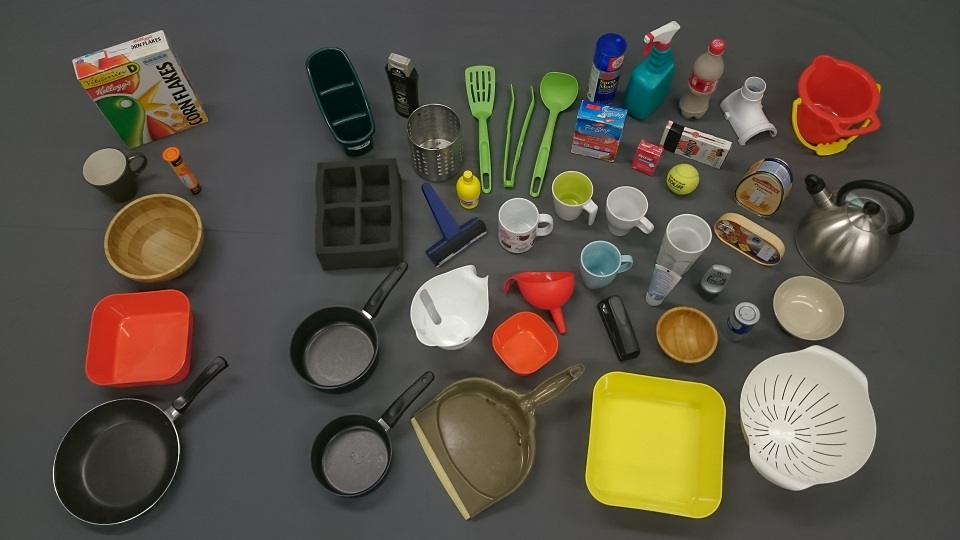
\includegraphics[width=0.7\linewidth]{images/objects.jpg}
  \end{center}
  \caption{The real objects. The training objects are on the left, testing objects are on the right.}
  \label{fig:real-objects}
\end{figure}

\begin{table}[b]
\small
\begin{center}
\caption{Performance on the real robot. \label{tab:robot-results}}
\begin{tabular}{|c|c|c|c|c|c|} \hline
Alg & \# succ & \% succ & Alg & \# succ & \% succ \\ \hline
V1  &  28 & 57.1\% & V4   & 37  & 75.5\% \\
V2  & 40 & 81.6\% & V11 & 43  & 87.8\% \\
\hline
\end{tabular}
\end{center}
\end{table}

\begin{figure}[t]
\begin{center}
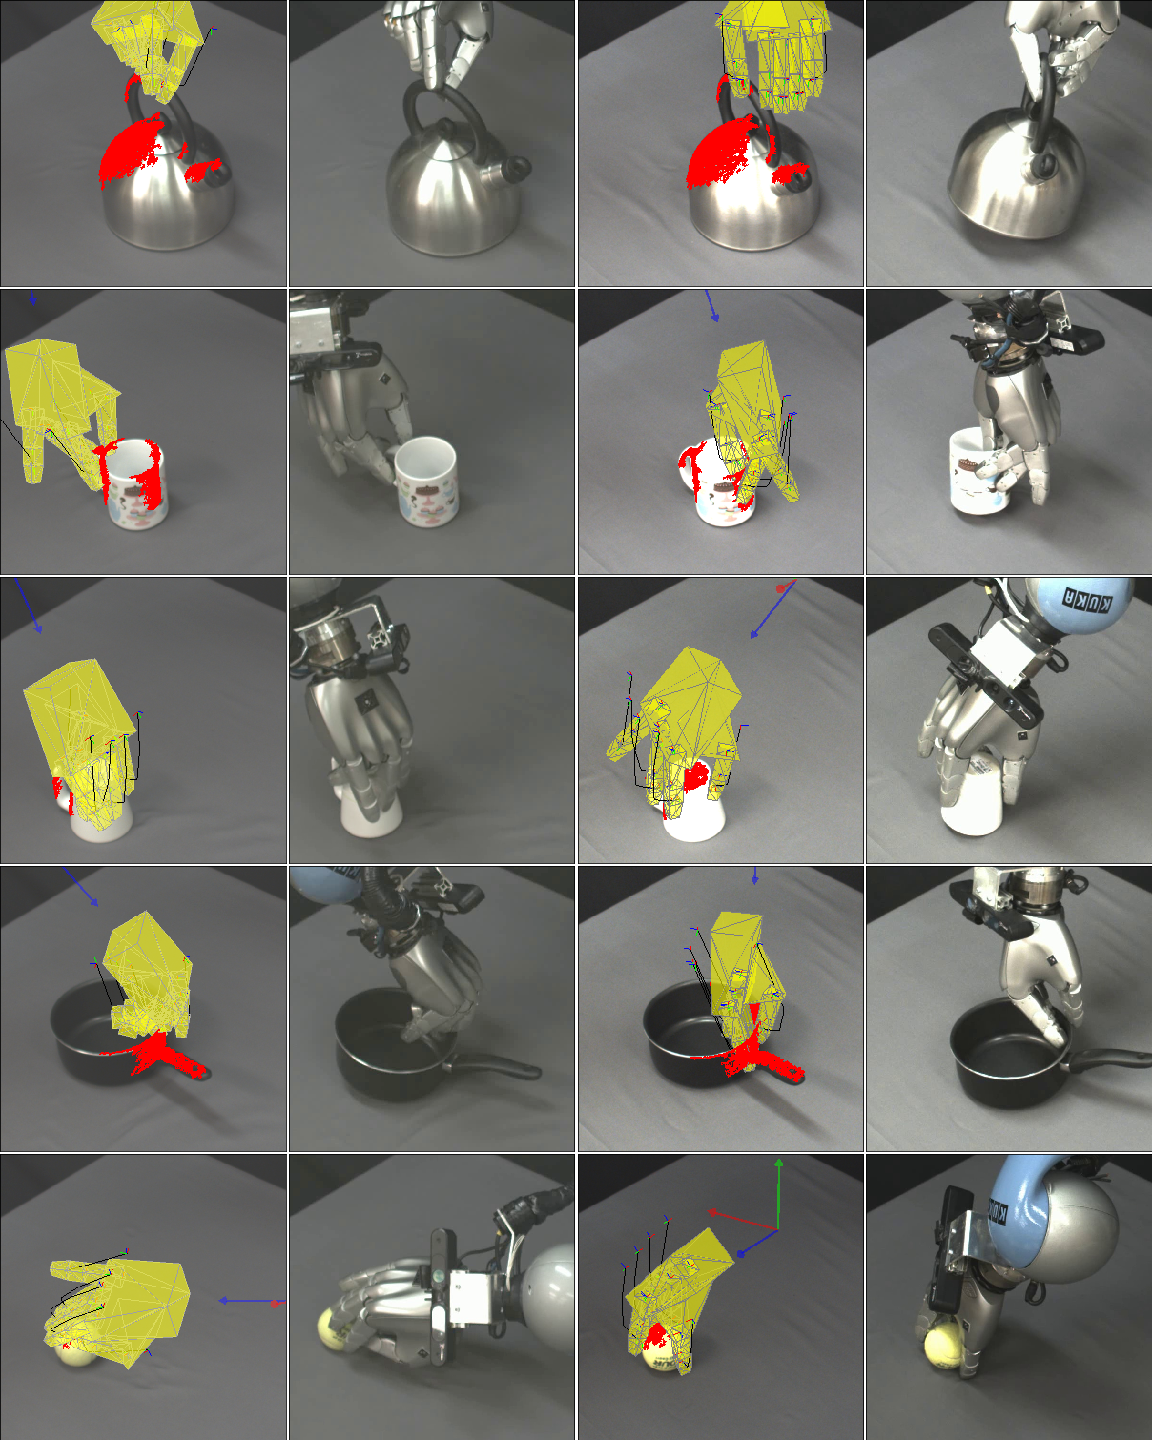
\includegraphics[width=0.5\columnwidth]{plots/A6fA10s_vertical.png}
\caption{V2 vs V11. This shows grasps from methods based on generative model GM2. The V2 grasps are shown in columns 1-2. The corresponding V11 grasps are shown in columns 3-4. These are the cases where V2 failed and V11 succeeded. \label{fig:v2fv11s}}
\end{center}
\end{figure}

\begin{figure}[t]
\begin{center}
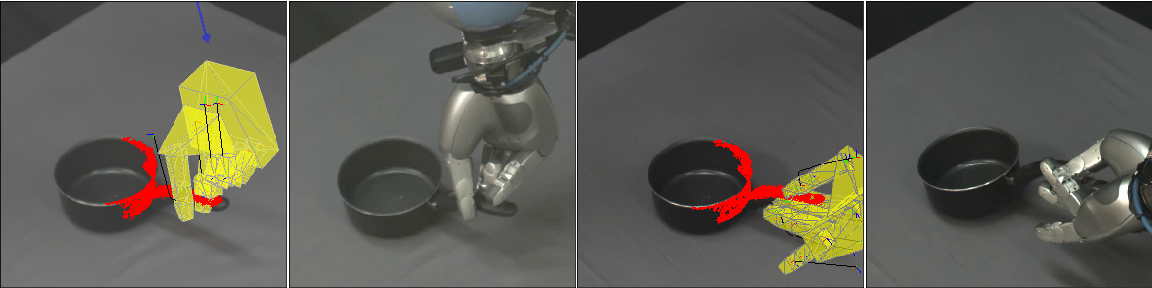
\includegraphics[width=0.5\columnwidth]{plots/A6fA10f_vertical.png}\\
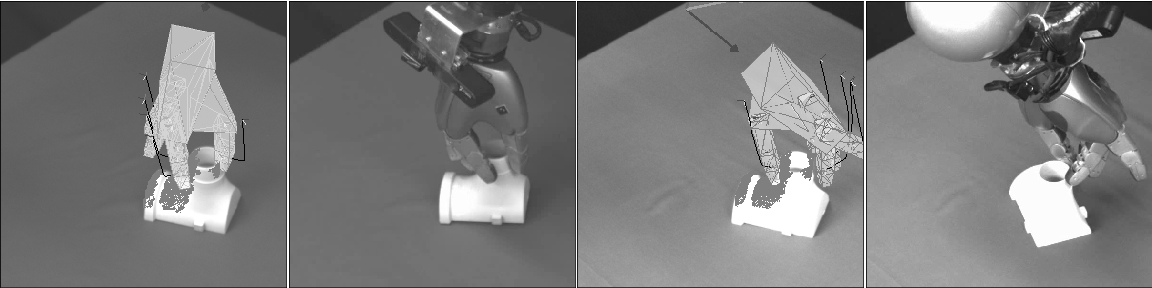
\includegraphics[width=0.5\columnwidth]{plots/A6sA10f_vertical.png}
\caption{V2 vs V11. This shows grasps from methods based on generative model GM2. The V2 grasps are shown in columns 1-2. The corresponding V11 grasps are shown in columns 3-4. The top row shows the case where both failed. The bottom row shows the case where V2 succeeded and V11 failed. \label{fig:v2fsv11f}}
\end{center}
\end{figure}


We compared four variants on the real robot: V1, V2, V4 and V11. V1 and V2 are the pure generative models. V4 is, in simulation, the equal best generative-evaluative method using GM1 as the generative model. It uses EM2 as the evaluative model. V11 is, in simulation, the best performing generative-evaluative method using GM2 as the generative model. This selection allows us to compare the best generative-evaluative methods with their counterpart pure generative models. 

We employed the same real objects as described in \cite{kopicki2019ijrr}. This used 40 novel test objects (Figure~\ref{fig:real-objects}). Object-pose combinations were chosen to reduce the typical surface recovery. Some objects were employed in several poses, yielding 49 object-pose pairs. From the 40 objects, 35 belonged to object classes in the simulation dataset, while the remaining five did not. 

Using this data-set, all algorithms were evaluated on the real-robot using a paired trials methodology. Each was presented with the same object-pose combinations. Each variant generated a ranked list of grasps, and the highest ranked grasp was executed. The highest-ranked grasp based on the predicted success probability of an evaluative network is performed on each scene. A grasp was deemed successful if, when lifted for five seconds, the object then remained stable in the hand for a further five seconds. 

The results are shown in Table~\ref{tab:robot-results}. In each case, the generative-evaluative variant outperforms the equivalent pure GM variant. So that V4 outperforms V1 by 75.5\% grasp success rate to 57.1\% and V11 outperforms V2 87.8\% to 81.6\%. The differences between V11:V1 and V2:V1 are highly statistically significant ($p<0.01$) using McNemar's test. Thus, we have strong support for our main hypothesis, which is that a Generative-Evaluative architecture outperforms a pure generative model. Six of the available grasp types were deployed (pinch support, pinch, pinchbottom, rimside, rim and power edge), showing that a variety of grasps is utilised.
%The success rate for GM1 was 57.1\% and for the top-performing method based on GM1, GEA.1, it was 77.6\% (Table~\ref{tab:robot-results}). The success rate of the second baseline, GM2, is 81.6\%, while GEA.3 shows outperforms it with a success rate of 87.8\%. A two-tailed McNemar test, for the difference between success rates for paired comparison data, was performed. The difference between the two algorithms has a $p$-value of 0.0442, and so is statistically significant. A selection of grasps where the two methods performed differently are shown in Figure~\ref{fig:successfail}.

% OLD TABLE
%\begin{table}
%\begin{center}
%\caption{Results of the real robot paired comparison trial.}
%\begin{tabular}{|c|c|c|c|}  \hline 
%          &                & \multicolumn{2}{ c |}{ GM} \\ \hline
%          &                & \# succs & \# fails  \\  \hline
 %GEA  & \# succs &  23 &  15  \\
 %         & \# fails    &  5   &   6   \\ \hline
%\end{tabular}
%\end{center}
%\label{tab:robot-results}
%\end{table}

%\begin{table}
%\begin{center}
%\caption{Results of the real robot paired comparison trial.}
%\label{my-label}
%\begin{tabular}{|cc|c|c|l}
%\cline{1-4}
%                                           &         & \multicolumn{2}{c|}{GM} &  \\ \cline{3-4}
%                                           &         & \# succs    & \# fails    &  \\ \cline{1-4}
%\multicolumn{1}{|c|}{\multirow{2}{*}{GEA}} & \# succs & 23         & 15         &  \\
%\multicolumn{1}{|c|}{}                     & \# fails & 5          & 6          &  \\ \cline{1-4}
%\end{tabular}
%\end{center}
%\label{tab:robot-results}
%\end{table}

\begin{figure*}
\begin{center}
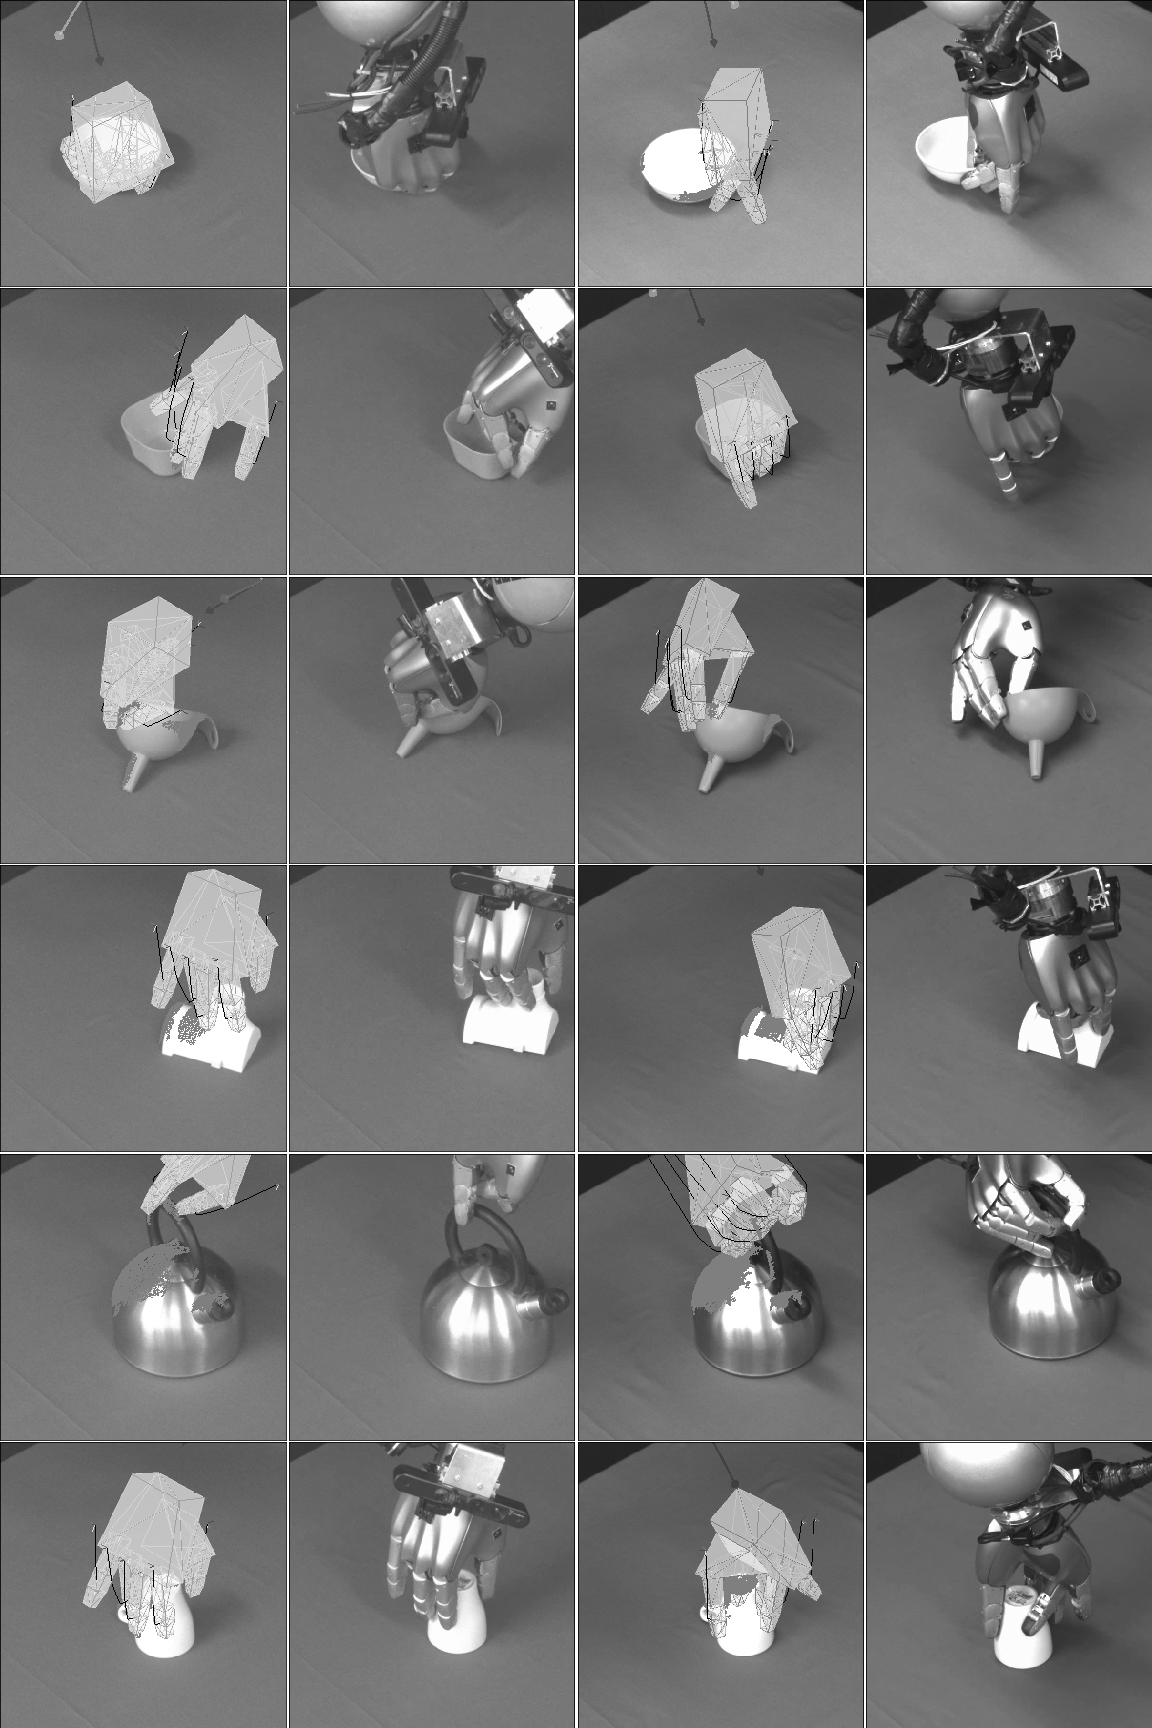
\includegraphics[width=0.48\textwidth]{plots/A2fA9s_1_vertical.png}~
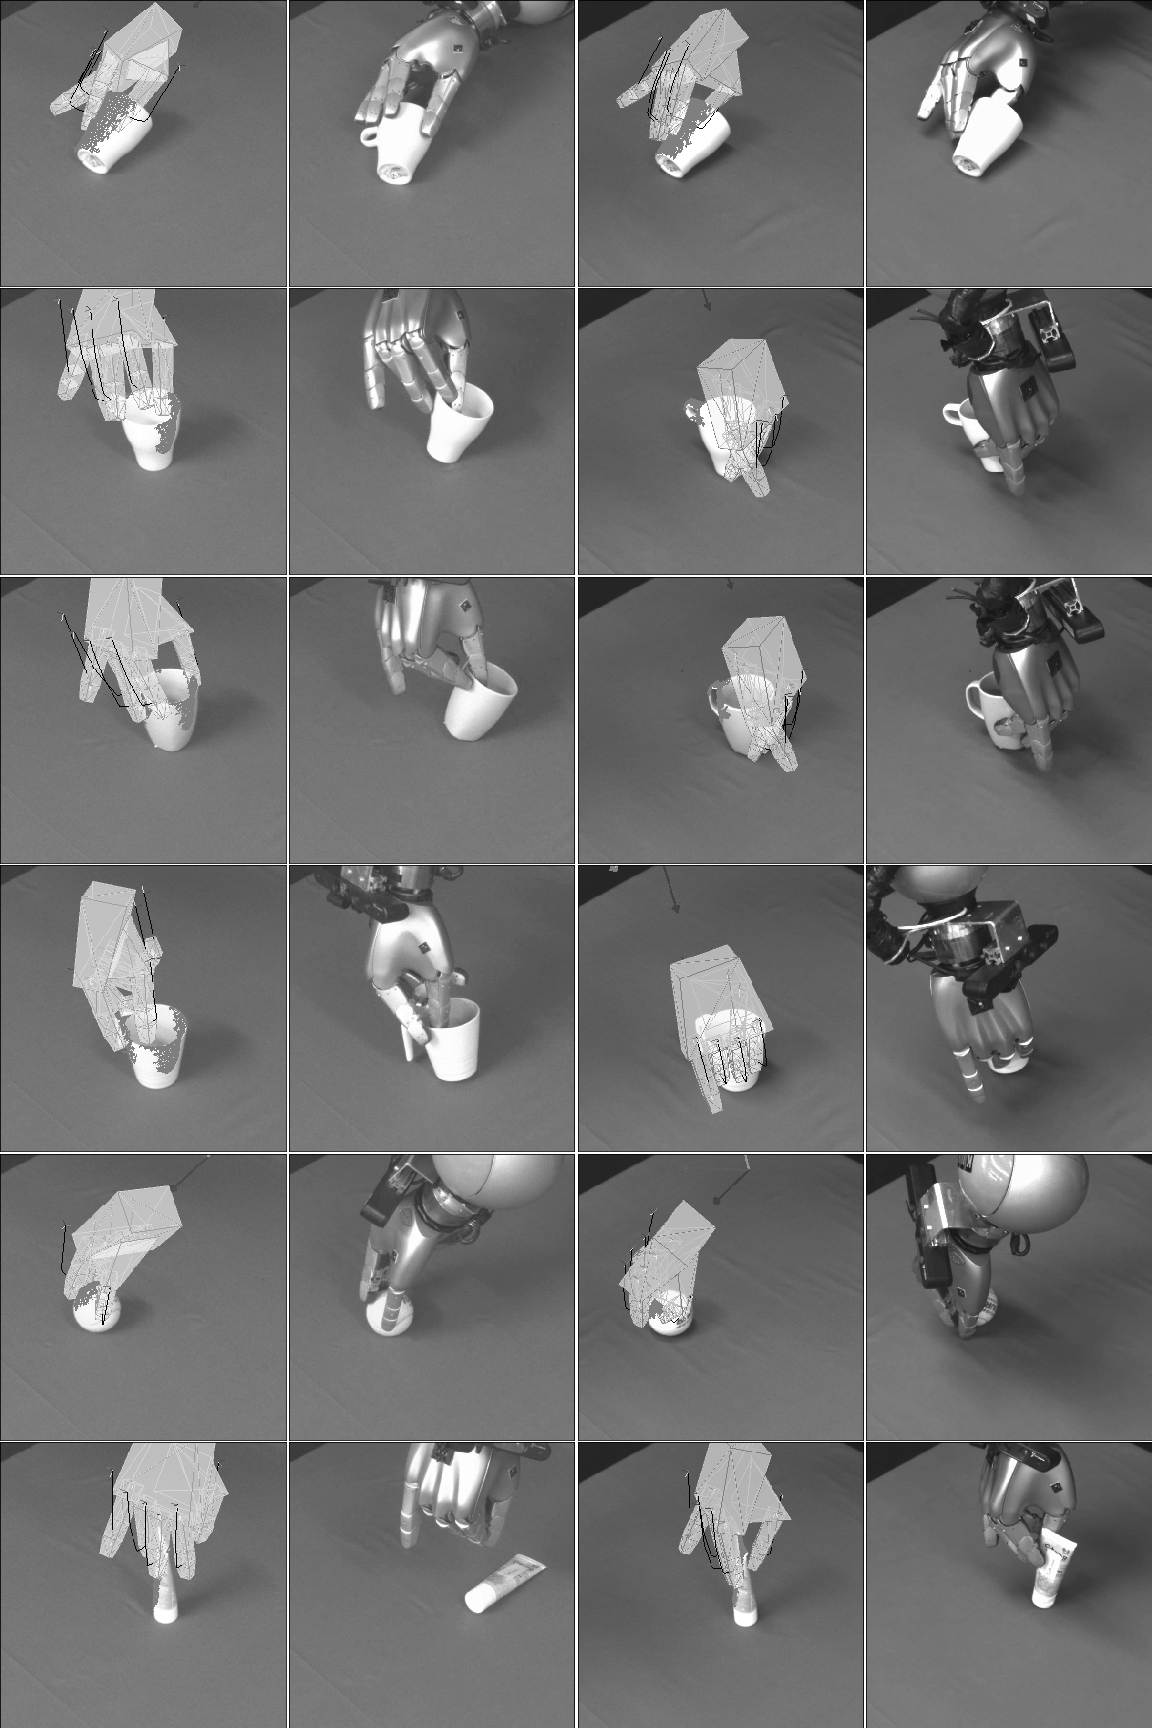
\includegraphics[width=0.48\textwidth]{plots/A2fA9s_2_vertical.png}
\caption{V1 vs V4. This shows grasps from methods based on generative model GM1. The V1 grasps are shown in columns 1-2 and 5-6. The corresponding V4 grasps are in columns 3-4 and 7-8. These are the cases where V1 failed and V4 succeeded.\label{fig:v1fv4s}}
\end{center}
\end{figure*}


\begin{figure*}
\begin{center}
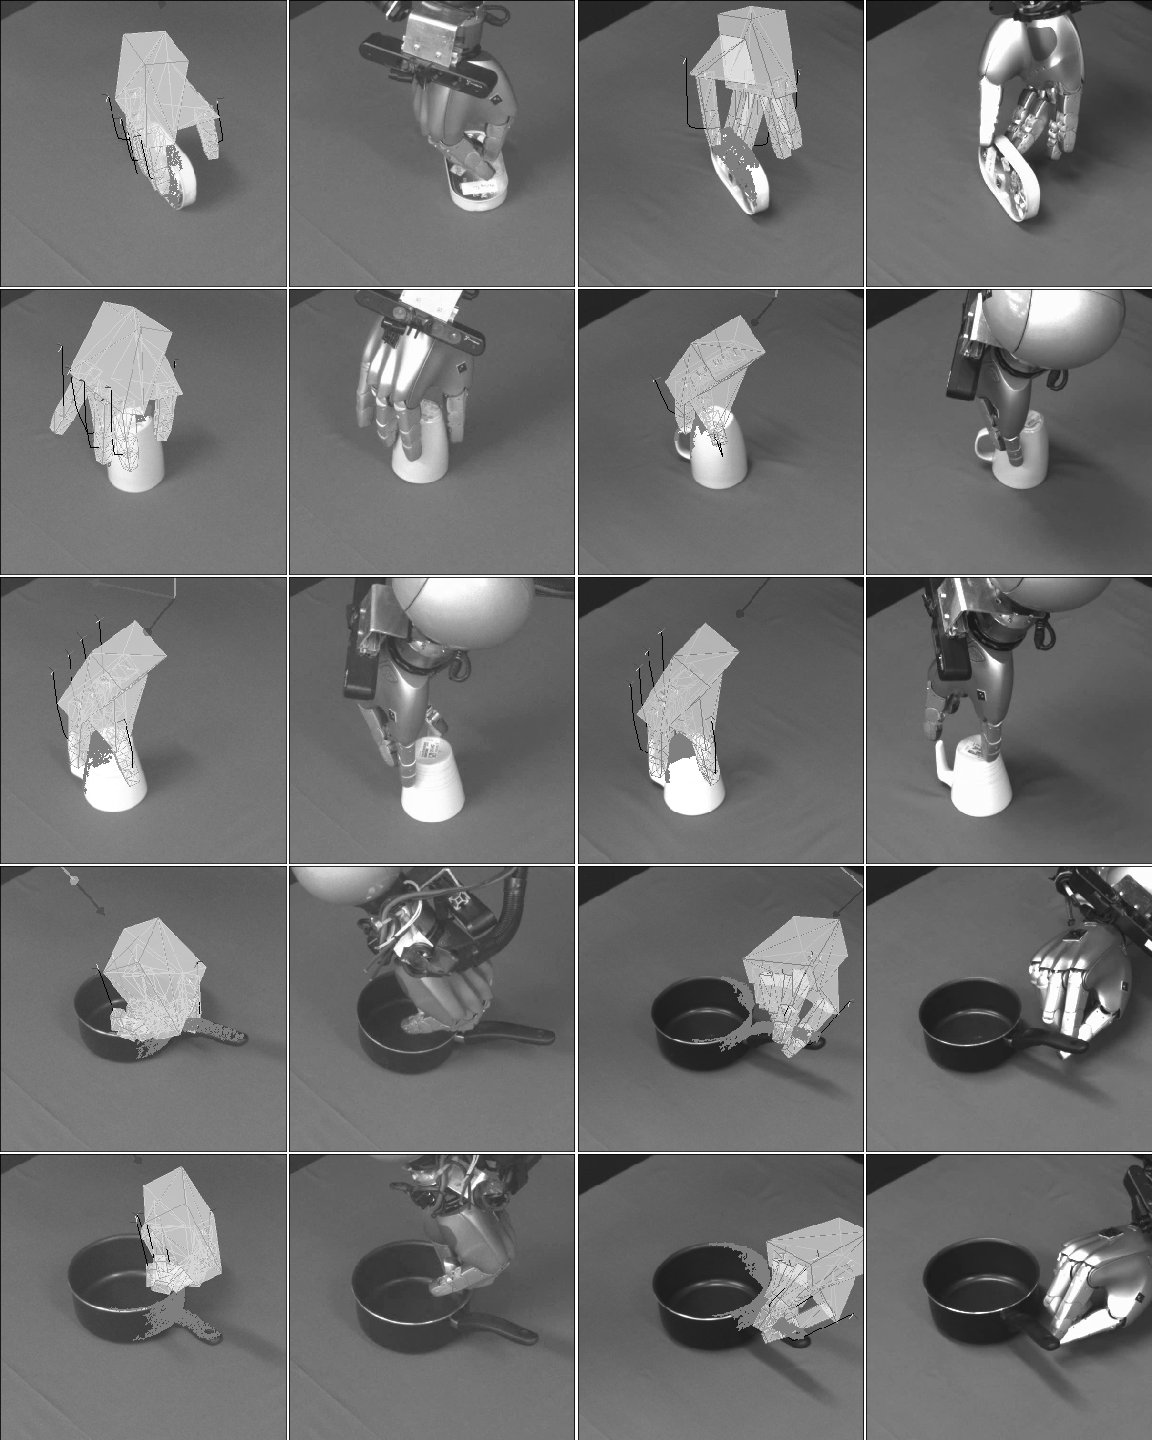
\includegraphics[width=0.48\textwidth]{plots/A2fA9f_vertical.png}~
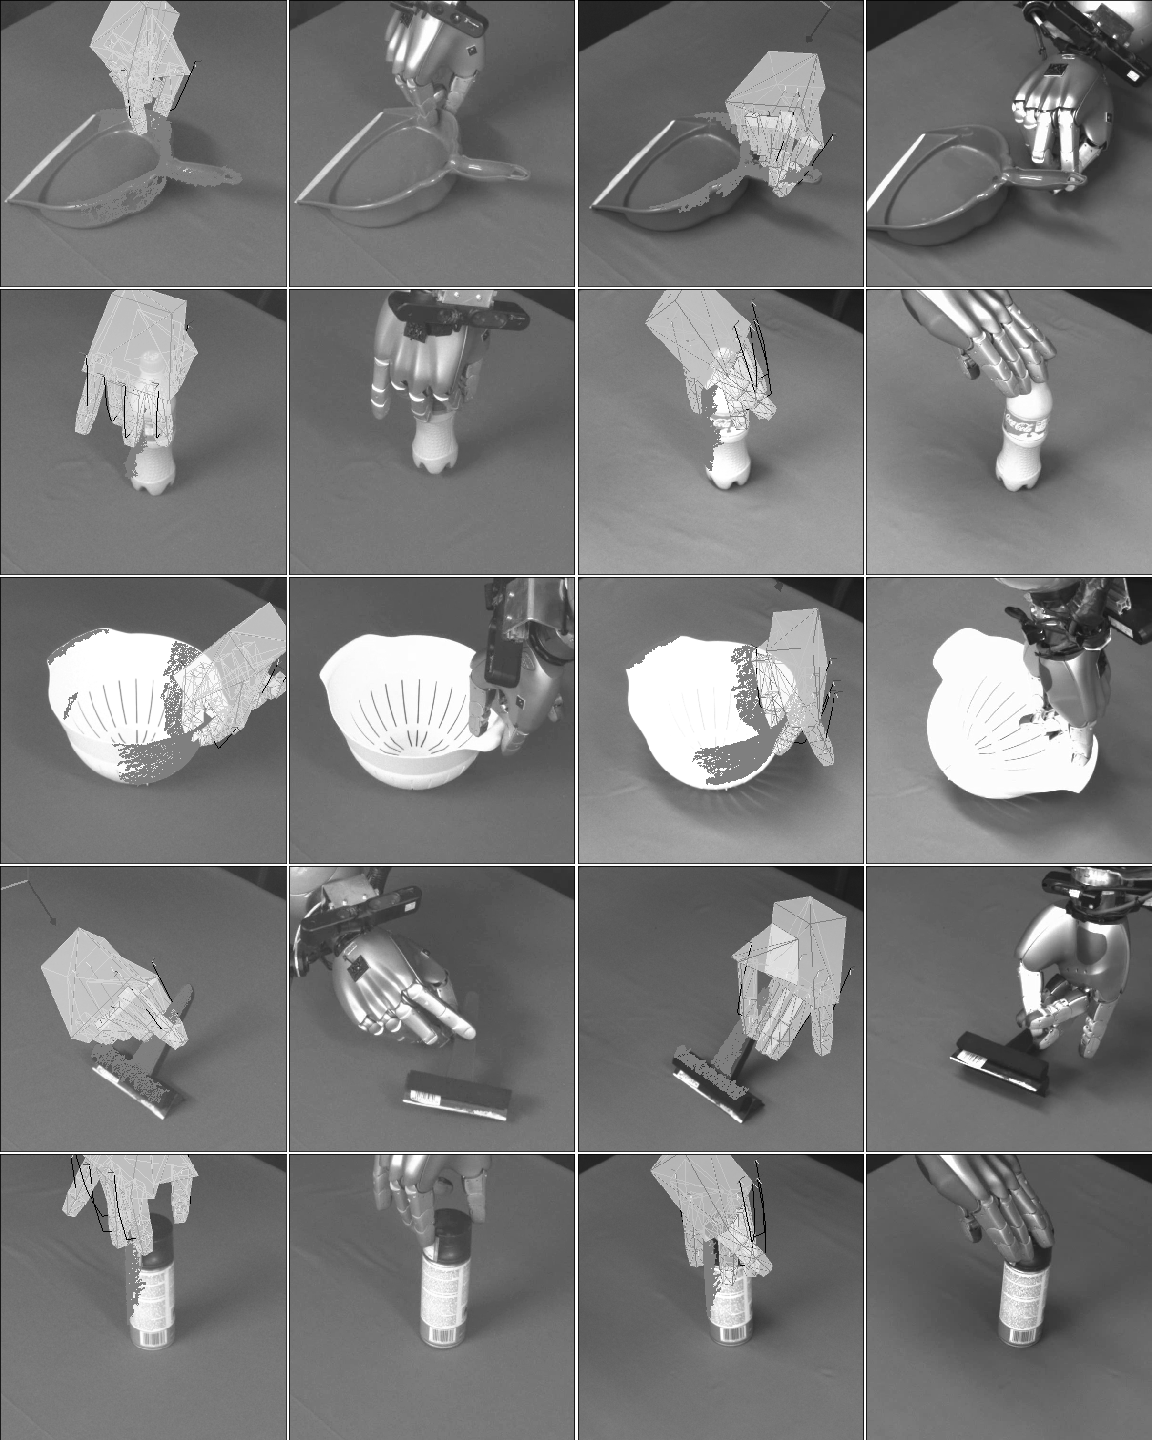
\includegraphics[width=0.48\textwidth]{plots/A2sA9f_vertical.png}
\caption{V1 vs V4. This shows grasps from methods based on generative model GM1. The V1 grasps are shown in columns 1-2 and 5-6. The corresponding V4 grasps are shown in columns 3-4 and 7-8. The left panel shows the cases where both V1 and V4 failed, while the right one shows the cases where V1 succeeded and V4 failed. \label{fig:v1fsv4f}}
\end{center}
\end{figure*}

%\begin{figure*}
%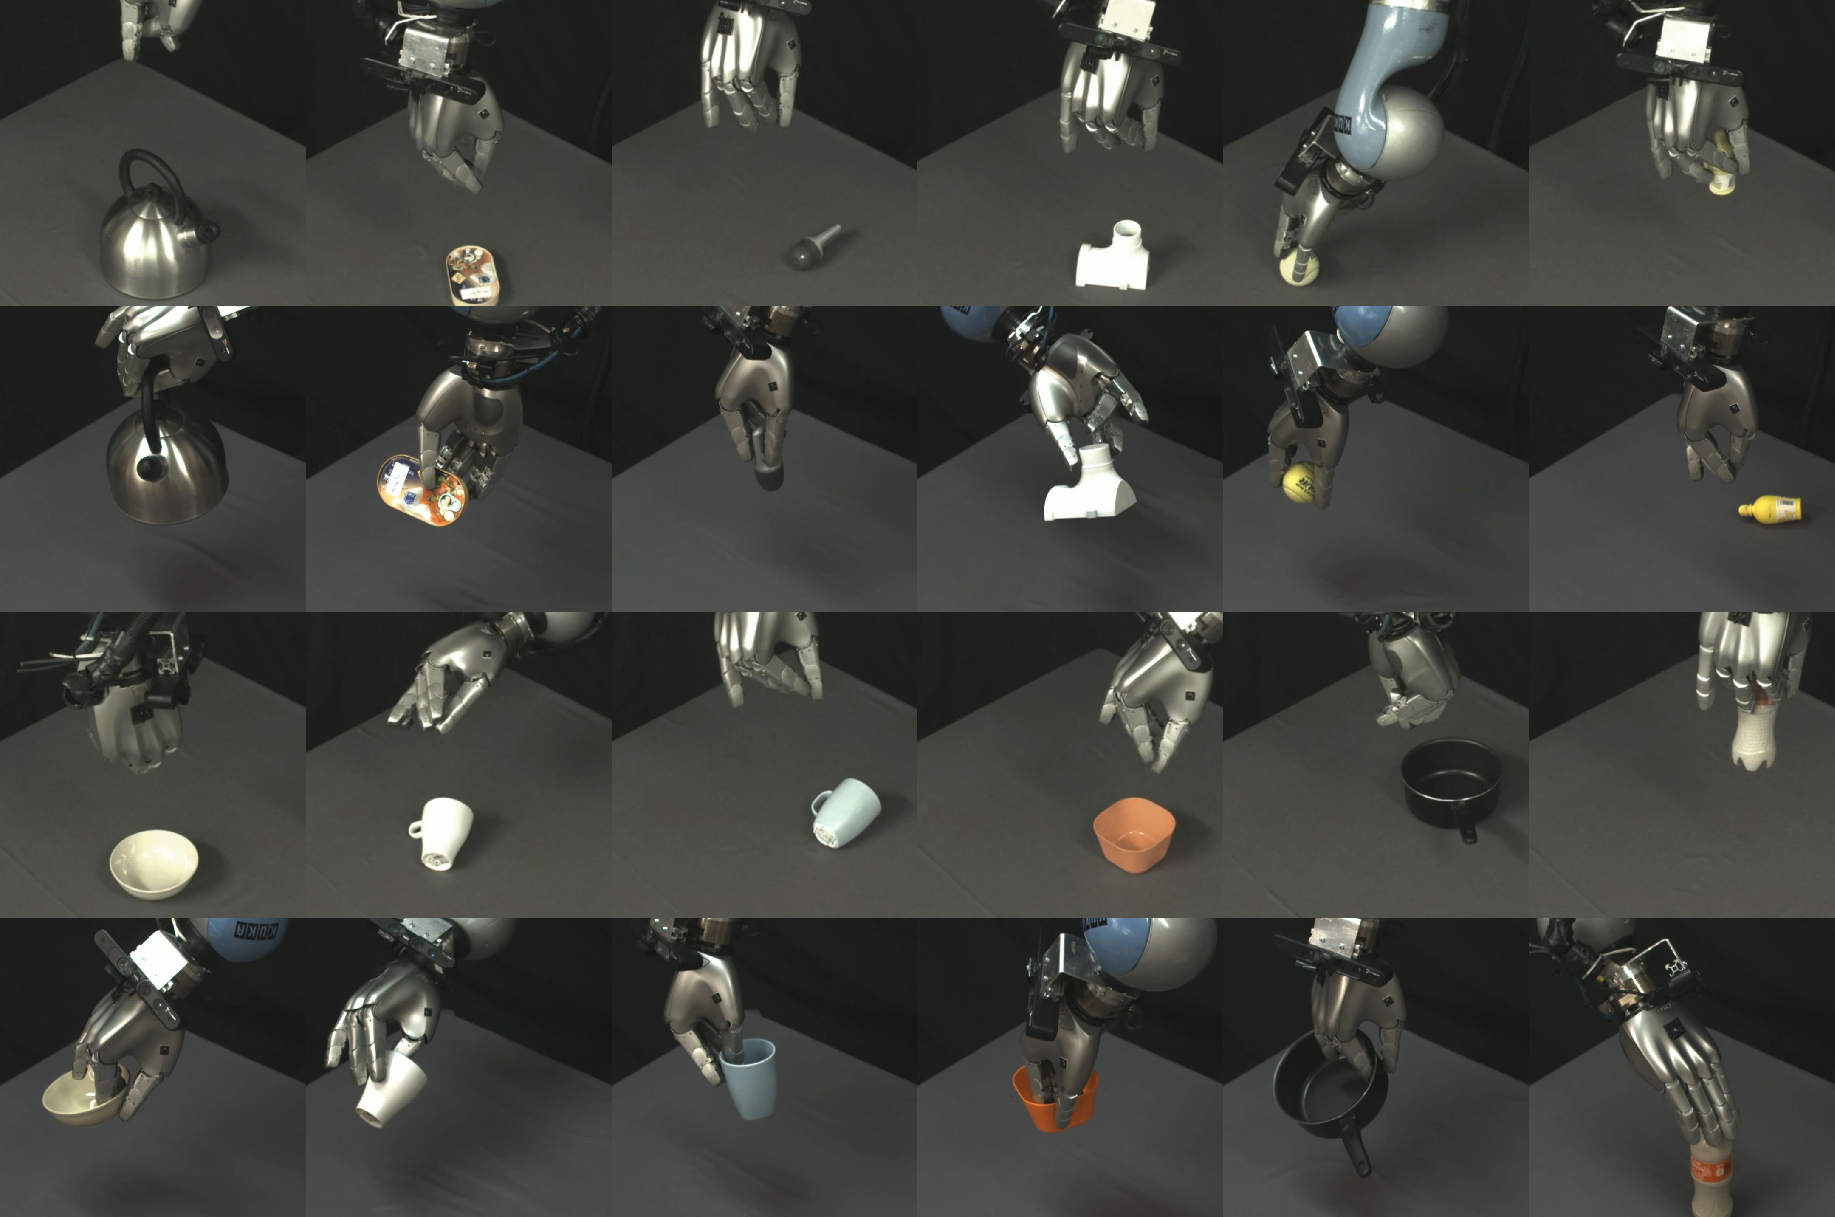
\includegraphics[width=\textwidth]{images/successfailure.pdf}
%\caption{Examples of grasps generated by the generative model (GM, $1^{st}$ and $3^{rd}$ row) and the generative-evaluative model (GEA, $2^{nd}$ and $4^{th}$ row) on paired trials. The first five columns show some of the 15 cases where the GEA model succeeds but GM fails. The far right-hand column shows 2 of the 5 converse cases. \label{fig:successfail}}
%\end{figure*}

%Training parameters for network. Training of example grasps for learning from demonstration. Creation of real test data set. Paired comparisons methodology with vanilla LFD algorithm (pose + object + camera view).
%
%The actual grasping tests have been performed on the real robot. 

\section{Conclusion} 
\label{sec:conclusion}
This paper has presented the first generative-evaluative architecture for dexterous grasping from a single view in which both the generative and evaluative models are learned. Using this architecture the success rate for the top ranked grasp rises from 69.5\% (for V1) to 90.49\% (for V11) on a simulated test set. It also presented a real robot data set where the top ranked grasp success rate rose from 57.1\% (V1) to 87.8\% (V11).

What are the promising lines of enquiry to further improve dexterous grasping of unfamiliar objects? We see three major issues. First, we have assumed no notion of object completion. Humans succeed in grasping in part because we have strong priors on object shape that help complete the missing information. This would enable the deployment of a generative model that exploits a more complete object shape model \cite{kopicki2015ijrr}. Second, our approach is open-loop during execution. For pinch-grasping, deep nets have been shown to learn useful visual servoing policies \cite{morrison18}. However, significant gains will also come from post-grasp force-control strategies, which are largely absent from the literature on grasp learning.  Third, the architectural scheme presented here is essentially that of an actor-critic architecture. This suggests incremental refinement of both the generative model and the evaluative model, perhaps using techniques from reward based learning. We have already shown elsewhere that the GM may be further improved by training from autonomously generated data \cite{kopicki2019ijrr}. Data intensive generative models also hold promise \cite{veres2017modeling} and it may be possible to seed them by training with example grasps drawn from a data-efficient model such as that presented here.


% An example of a floating figure using the graphicx package.
% Note that \label must occur AFTER (or within) \caption.
% For figures, \caption should occur after the \includegraphics.
% Note that IEEEtran v1.7 and later has special internal code that
% is designed to preserve the operation of \label within \caption
% even when the captionsoff option is in effect. However, because
% of issues like this, it may be the safest practice to put all your
% \label just after \caption rather than within \caption{}.
%
% Reminder: the "draftcls" or "draftclsnofoot", not "draft", class
% option should be used if it is desired that the figures are to be
% displayed while in draft mode.
%
%\begin{figure}[!t]
%\centering
%\includegraphics[width=2.5in]{myfigure}
% where an .eps filename suffix will be assumed under latex, 
% and a .pdf suffix will be assumed for pdflatex; or what has been declared
% via \DeclareGraphicsExtensions.
%\caption{Simulation results for the network.}
%\label{fig_sim}
%\end{figure}

% Note that the IEEE typically puts floats only at the top, even when this
% results in a large percentage of a column being occupied by floats.


% An example of a double column floating figure using two subfigures.
% (The subfig.sty package must be loaded for this to work.)
% The subfigure \label commands are set within each subfloat command,
% and the \label for the overall figure must come after \caption.
% \hfil is used as a separator to get equal spacing.
% Watch out that the combined width of all the subfigures on a 
% line do not exceed the text width or a line break will occur.
%
%\begin{figure*}[!t]
%\centering
%\subfloat[Case I]{\includegraphics[width=2.5in]{box}%
%\label{fig_first_case}}
%\hfil
%\subfloat[Case II]{\includegraphics[width=2.5in]{box}%
%\label{fig_second_case}}
%\caption{Simulation results for the network.}
%\label{fig_sim}
%\end{figure*}
%
% Note that often IEEE papers with subfigures do not employ subfigure
% captions (using the optional argument to \subfloat[]), but instead will
% reference/describe all of them (a), (b), etc., within the main caption.
% Be aware that for subfig.sty to generate the (a), (b), etc., subfigure
% labels, the optional argument to \subfloat must be present. If a
% subcaption is not desired, just leave its contents blank,
% e.g., \subfloat[].


% An example of a floating table. Note that, for IEEE style tables, the
% \caption command should come BEFORE the table and, given that table
% captions serve much like titles, are usually capitalized except for words
% such as a, an, and, as, at, but, by, for, in, nor, of, on, or, the, to
% and up, which are usually not capitalized unless they are the first or
% last word of the caption. Table text will default to \footnotesize as
% the IEEE normally uses this smaller font for tables.
% The \label must come after \caption as always.
%
%\begin{table}[!t]
%% increase table row spacing, adjust to taste
%\renewcommand{\arraystretch}{1.3}
% if using array.sty, it might be a good idea to tweak the value of
% \extrarowheight as needed to properly center the text within the cells
%\caption{An Example of a Table}
%\label{table_example}
%\centering
%% Some packages, such as MDW tools, offer better commands for making tables
%% than the plain LaTeX2e tabular which is used here.
%\begin{tabular}{|c||c|}
%\hline
%One & Two\\
%\hline
%Three & Four\\
%\hline
%\end{tabular}
%\end{table}


% Note that the IEEE does not put floats in the very first column
% - or typically anywhere on the first page for that matter. Also,
% in-text middle ("here") positioning is typically not used, but it
% is allowed and encouraged for Computer Society conferences (but
% not Computer Society journals). Most IEEE journals/conferences use
% top floats exclusively. 
% Note that, LaTeX2e, unlike IEEE journals/conferences, places
% footnotes above bottom floats. This can be corrected via the
% \fnbelowfloat command of the stfloats package.





% if have a single appendix:
%\appendix[Proof of the Zonklar Equations]
% or
%\appendix  % for no appendix heading
% do not use \section anymore after \appendix, only \section*
% is possibly needed

% use appendices with more than one appendix
% then use \section to start each appendix
% you must declare a \section before using any
% \subsection or using \label (\appendices by itself
% starts a section numbered zero.)
%


%\appendices
%\section{Proof of the First Zonklar Equation}
%Appendix one text goes here.

% you can choose not to have a title for an appendix
% if you want by leaving the argument blank
%\section{}
%Appendix two text goes here.


% use section* for acknowledgment
\section*{Acknowledgment}

The authors gratefully acknowledge funding from the European Commission Funded project, PaCMan FP7-IST-600918.


% Can use something like this to put references on a page
% by themselves when using endfloat and the captionsoff option.
\ifCLASSOPTIONcaptionsoff
  \newpage
\fi



% trigger a \newpage just before the given reference
% number - used to balance the columns on the last page
% adjust value as needed - may need to be readjusted if
% the document is modified later
%\IEEEtriggeratref{8}
% The "triggered" command can be changed if desired:
%\IEEEtriggercmd{\enlargethispage{-5in}}

% references section

% can use a bibliography generated by BibTeX as a .bbl file
% BibTeX documentation can be easily obtained at:
% http://mirror.ctan.org/biblio/bibtex/contrib/doc/
% The IEEEtran BibTeX style support page is at:
% http://www.michaelshell.org/tex/ieeetran/bibtex/
%\bibliographystyle{IEEEtran}
% argument is your BibTeX string definitions and bibliography database(s)
%\bibliography{IEEEabrv,../bib/paper}
%
% <OR> manually copy in the resultant .bbl file
% set second argument of \begin to the number of references
% (used to reserve space for the reference number labels box)
\bibliographystyle{IEEEtran}
\bibliography{new_total}%,newbib,main,deepgrasping,references,some_references_by_Chao}

% biography section
% 
% If you have an EPS/PDF photo (graphicx package needed) extra braces are
% needed around the contents of the optional argument to biography to prevent
% the LaTeX parser from getting confused when it sees the complicated
% \includegraphics command within an optional argument. (You could create
% your own custom macro containing the \includegraphics command to make things
% simpler here.)
%\begin{IEEEbiography}[{\includegraphics[width=1in,height=1.25in,clip,keepaspectratio]{mshell}}]{Michael Shell}
% or if you just want to reserve a space for a photo:

%\begin{IEEEbiography}{Michael Shell}
%Biography text here.
%\end{IEEEbiography}

% if you will not have a photo at all:
%\begin{IEEEbiographynophoto}{John Doe}
%Biography text here.
%\end{IEEEbiographynophoto}

% insert where needed to balance the two columns on the last page with
% biographies
%\newpage

%\begin{IEEEbiographynophoto}{Umit Rusen Aktas}
\begin{IEEEbiography}
[{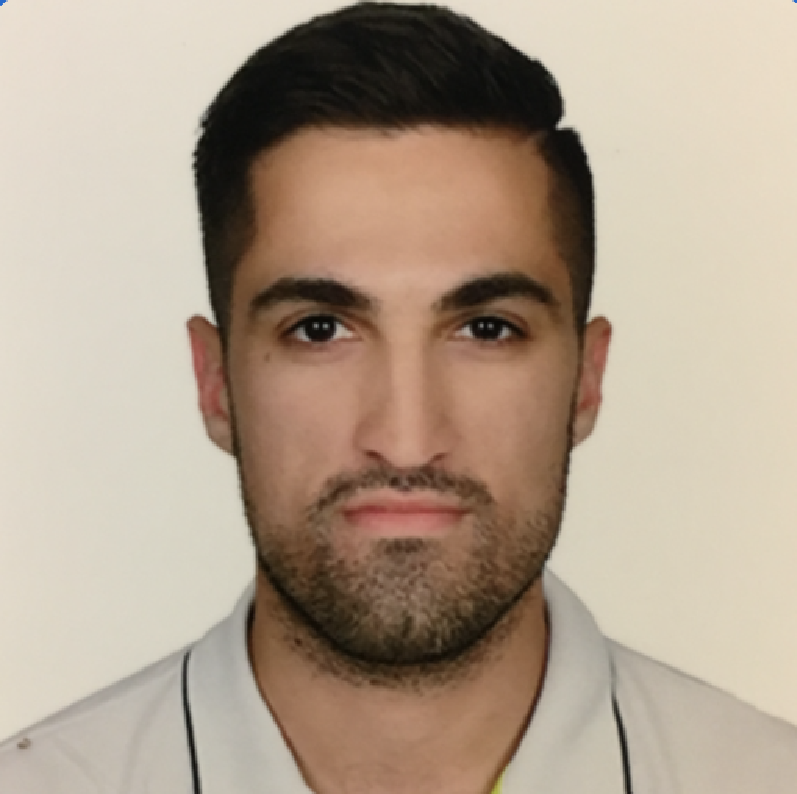
\includegraphics[width=1in,height=1.25in,clip,keepaspectratio]{images/bio/rusen_bio}}]{Umit Rusen Aktas}
Umit Rusen Aktas is currently working as a Research Engineer for Blue Prism in London. He got his PhD in Computer Science from University of Birmingham in 2018. He received a BSc and MSc in Computer Engineering from METU, Ankara in 2010 and 2013, respectively. His research interests include deep networks, robot vision, graph theory and computer graphics. 
\end{IEEEbiography}

\begin{IEEEbiography}
[{\includegraphics[width=1in,height=1.25in,clip,keepaspectratio]{images/bio/dummy}}]{Chao Zhao}
Bla bla bla
\end{IEEEbiography}

\begin{IEEEbiography}
[{\includegraphics[width=1in,height=1.25in,clip,keepaspectratio]{images/bio/dummy}}]{Marek Kopicki}
Bla bla bla
\end{IEEEbiography}

\begin{IEEEbiography}
[{\includegraphics[width=1in,height=1.25in,clip,keepaspectratio]{images/bio/dummy}}]{Ales Leonardis}
Bla Bla Bla
\end{IEEEbiography}

\begin{IEEEbiography}
[{\includegraphics[width=1in,height=1.25in,clip,keepaspectratio]{images/bio/dummy}}]{Jeremy L. Wyatt}
Bla Bla Bla
\end{IEEEbiography}

% You can push biographies down or up by placing
% a \vfill before or after them. The appropriate
% use of \vfill depends on what kind of text is
% on the last page and whether or not the columns
% are being equalized.

\vfill

% Can be used to pull up biographies so that the bottom of the last one
% is flush with the other column.
%\enlargethispage{-5in}



% that's all folks
\end{document}


